\chapter{Standard Model Backgrounds}
\label{chap:backgrounds}

\section{Common Background Estimation and Validation Techniques}
\label{sec:Bkg:Tech}

\indent We use both data and MC based background estimation technique for estimating background in the signal region.  A common partially data driven technique is by using different control regions (CR) to directly measure the amount of background from data.  Once we know the amount of background in the CR, we can then extrapolate to the signal region using MC predictions of the relative amount of background in CR and SR. 

\indent The total amount of background is determined through a simultaneous fit to SR and all CRs.  The background rate will be mainly constrained by the CRs because the CR contain many more events the SR and is pure in specific types of background.  A more detailed explanation of CR, SR and fits are covered in the statistical analysis section \ref{sec:stat:Bkg}.  \\

\indent Aside from the fitting to control regions, we can get a simplified estimate of the amount of background in the SR through a simpler method.  We can calculate the transfer factor and normalization factor defined in equation \ref{eqn:TF} and \ref{eqn:mu}. This simplified result may slightly differ for the combined fit but should be similar as long as the CRs are well designed and consists mainly of a single type of background. \\

\begin{equation}
T = \frac{N_{MC}^{SR}}{N_{MC}^{CR}}
\label{eqn:TF}
\end{equation}
\begin{equation}
\mu_{MC} = \frac{N_{data}^{CR}-N_{non-ttbar MC}^{CR}}{N_{ttbar~MC}^{CR}}
\label{eqn:mu}
\end{equation}

\indent We normalize the ttbar MC in the ttbar CR to the amount of data with a normalization scale factor $\mu$ defined in equation \ref{eqn:mu}.  We then apply the transfer factor to predict the amount of ttbar we expect to see in the SR.  This is mathematically equivalent to simply normalizing the amount of ttbar MC in the SR by the scale factor derived in the CR because the transfer factor is the just the relative rates of MC in the SR and CR.   \\

\indent We use control regions to estimate the dominant ttbar background and subdominant W+jet, single top, and ttV backgrounds.  Z+jets and diboson backgrounds are estimated using MC alone.  Z+jets and diboson contributions are less then 5 percent of all backgrounds in the SR and we allow for an additional 100 percent theory uncertainty for these two samples.  Details on the ttbar background is found in section \ref{sec:Bkg:ttbar}. Details on the treatment of each sub dominate background can be found in section \ref{sec:Bkg:sub}. Finally QCD multijet background is estimated using the jet smearing method described in section \ref{sec:Bkg:QCD}. \\

\indent The scale factors for each background derived from the simultaneous fit to the CR are given in table \ref{table.scale.factors}. ttbar background is scaled down by 0.707 because the MC over estimates the amount of ttbar that is produced with strong ISR. \\

\begin{table}
  \begin{center}
    \begin{tabular*}{\textwidth}{@{\extracolsep{\fill}}lr}
      \noalign{\smallskip}\hline\noalign{\smallskip}
      {\bf MC sample}           & Fitted scale factor        \\[-0.05cm] \hline
      ttbar &   $0.707 \pm 0.050$             \\
      W+jets &   $1.27 \pm 0.15$              \\
      Single top &   $1.17 \pm 0.39$              \\
      ttbar$\gamma$ &   $1.29 \pm 0.20$              \\ \hline
    \end{tabular*}

  \end{center}
  \caption{MC scale factors for SM backgrounds.  Scale factors are derived by simultaneously fitting to all background CR using \intlumi\ \ifb of data.}
  \label{table.scale.factors}
\end{table}

\section{Dominant Background: Standard Model $t\tbar$}
\label{sec:Bkg:ttbar}

\indent The dominant background in this analysis is SM ttbar.  After signal selection ttbar still accounts for $70$-$90$ percent of the background depending on the $\RISR$ range.  This section covers in detail the properties and treatment of SM ttbar in this analysis.  The section \ref{sec:Bkg:ttbar:Pop} demonstrates that there exists two kinematically distinct populations of SM ttbar, each with unique characteristics and observables.  Section \ref{sec:Bkg:ttbar:CR} describes how we are able to directly measure the amount of ttbar in SR using a one lepton CR.  \\

%Section \ref{sec:Bkg:ttbar:Sel} explores the kinematics of ttbar events after SR selection.  

%\indent The $\met>250 \gev$ requirement selects ttbar with boosted leptonic tops because a top at rest cannot produce a neutrino with 250 $\gev of $\pt$.  After zero lepton preselection, two kinematically distinct populations of ttbar exist.  One ttbar population use strong ISR to boost both tops. The other population uses boosts the leptonic top against the hadronic top in a back to back fashion. Section \ref{sec:Bkg:ttbar:Pop} describes these two kinematically distinct populations of ttbar in greater detail.   \\

%\indent Section \ref{sec:Bkg:ttbar:Sel} describes the signal selections used to remove the majority of ttbar background while retaining most of the signal.  These selection targets the larger and kinematically different population of ttbar that does not have strong initial state radiation.  ttbar with strong ISR appears more signal like and 90 percent of all ttbar backgrounds after signal region selection are ttbar events with at least $400$ GeV of true initial state radiation.  These same selections are also very effective at removing sub-dominate SM backgrounds such as W+jets and Z+jets. \\

%\indent Section \ref{sec:Bkg:ttbar:CR} describes how we are able to directly measure the amount of ttbar background that is produced with strong initial state radiation in data using an one lepton control region.  We avoid relying on theory predictions on the amount of ISR ttbar is expected to produce.  In this way, the control region allows us to minimize the amount of systematic uncertainties in the signal region. \\

\subsection{Two Kinematically Distinct Populations of $t\tbar$}
\label{sec:Bkg:ttbar:Pop}

\indent After the zero lepton preselection, 80 percent of ttbar events decay via the single hadronic tau channel.  $15$ percent of ttbar events decay via the single lepton channel where the lepton is an electron or a muon.  The lepton is later lost because either it has too low pt to be reconstructed, removed because they were to close to another jet or is mis-reconstructed as a jet. The rest of the five percent are due to di-leptonic decays. Fully hadronic ttbar is negligible after SR selections because they produce little intrinsic $\met$. \\

\indent  The $\met>250 \gev$ requirement in preselection selects ttbar with boosted leptonic tops.  A top at rest simply do not have enough energy to produce a neutrino with 250 $\gev$ of $\pt$. The leptonic top can gain boost mainly through one of two ways.  Either the leptonic top recoils in a back to back fashion against the hadronic top or both tops can recoil against strong ISR.  \\

%\indent Most ttbar events has one top that decays leptonically and the other top decaying fully hadronically after zero lepton preselection. The leptonic top also produces a neutrino that satisfies the $250$ GeV of \MET requirement.  In most cases, the lepton is a tau that decays hadronically and registers as jet in calorimeter instead of a lepton.  In a smaller fraction of events a muon or electron is produced but the lepton is lost because of a number of reasons.  For example, the lepton can have too low pt to be reconstructed, or can be removed because they were to close to another jet or an electron is mis-reconstructed as a jet.  \\

%\indent Regardless of the exact decay channel, a top decaying at rest cannot generate enough momenta for the neutrino to have $250$ GeV of pt.  The top decaying via a tau or lepton, called the leptonic top, must therefore be boosted to have a high probability of satisfying the $250$ GeV \MET cut.  The leptonic top can gain this boost through one of two ways.  Either the leptonic top recoils in a back to back fashion against the hadronic top or both tops recoil against strong ISR.  \\

\indent In both situations the axis of maximum back to back $\pt$, the thrust axis, contains important information.  In the case where the leptonic is recoiling against the hadronic top, the thrust axis lines up along the top/anti-top's axis of back to back recoil.  In the case where both tops are boosted by strong ISR, the thrust axis approximates the ttbar vs ISR recoil direction. An artistic representation of the role of the thrust axis in each ttbar population can be seen in figure \ref{fig:ttbar:2pop}. \\

\begin{figure}[h!]
  \centering
	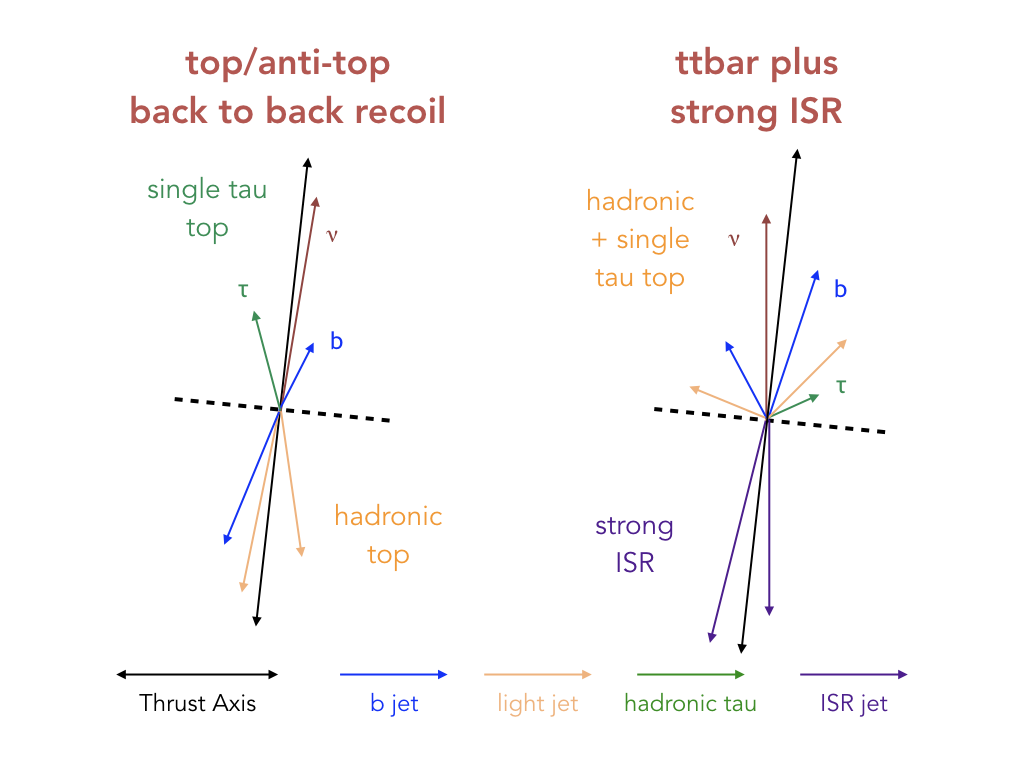
\includegraphics[width=0.65\textwidth]{./figures/strategy/ttbar_2pop.png}
	\caption{\label{fig:ttbar:2pop}{Depiction of the kinematics of the back to back ttbar population and the ttbar plus strong ISR population that exists after the zero lepton pre-selection. The two example event's thrust axis are aligned.  The hemisphere containing $\met$ has significantly higher jet multiplicities and total energy in ttbar plus strong ISR events. }}
\end{figure}

\indent The ttbar plus strong ISR population has on average much higher jet multiplicities and total energy in the hemisphere containing $\met$.  Hence, we can use observable such as $\NjV$ and $\MS$ to distinguish ttbar plus strong ISR events from top/anti-top back to back recoil events.   \\

%\subsection{Properties of SM $t\tbar$ in Signal Region}
%\label{sec:Bkg:ttbar:SR}

%\indent Stop signal is expected to have a higher jet multiplicities and energy in the hemisphere containing $\met$ then both ttbar populations.  The stringent SR requirements on the jet multiplicities and total energy of the sparticle hemisphere effectively eliminate the top/anti-top back to back ttbar population and also rejects approximately $2/3$ of ttbar plus strong ISR population.  A detailed explanation of SR design and performance can be found in chapter \ref{chap:SignalRegion}. \\

%\indent The ttbar events that survives the SR selections are composed of almost exclusively ttbar that are also produced with strong ISR.  Approximately 90 percent of the ttbar events in SR have an ISR pt of at least 400 $\gev$.  The distribution of true ISR pt for ttbar that survive the signal selections can be seen in figure \ref{fig:ttbar:SR:trueISRpt}.\\

%\begin{figure}[h!]
%  \centering
%	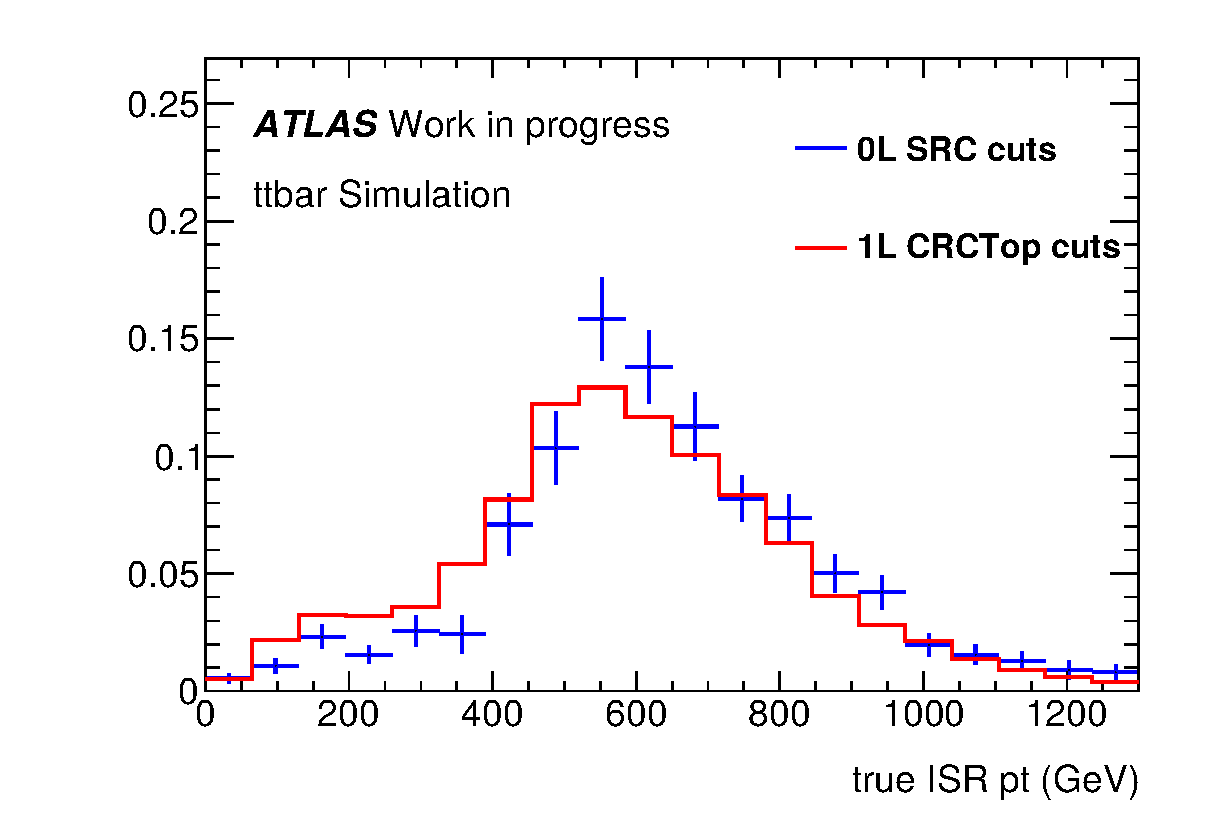
\includegraphics[width=0.65\textwidth]{./figures/ttbar/truePtISR_SRC_CRC_compare.eps}
%\caption{\label{fig:ttbar:CR:trueISRpt}{Distribution of true ISR pt for ttbar that survive the signal selections}}
%\end{figure}

%\indent In terms of branching fractions, the majority of ttbar branching fractions are to hadronic taus.  80 percent of the ttbar has one top decay via a single hadronic tau and the other top decays fully hadronically.  $15$ percent of the ttbar events decay via the single lepton channel where the lepton is an electron or a muon.  The lepton becomes lost because either it has too low pt to be reconstructed, removed because they were to close to another jet or is mis-reconstructed as a jet. The rest of the five percent composed of di-leptonic or lepton and tau ttbar events. Essentially no fully hadronic ttbar survives the zero lepton selection because fully hadronic ttbar do not make any hard neutrinos directly from the top decay.  \\
%\indent With such a large fraction of background coming from taus one might suspect setting up some sort of tau rejection.  However we found that a rejection based on loose tau IDs did not improve sensitivity.  The loss of signal was too large to justify the improvement in signal to background ratio.  The high jet multiplicity in signal gives a high probability of false positives.
%\indent Accepting mainly ttbar decay to hadronic taus gives a large boost signal to background due to branching fractions alone.  The two tops in signal events decay mainly through the fully hadronic channel.  Fully hadronic decays accounts for 44 percent of all ttbar decays.  On the other hand, the ttbar background mainly decay via hadronic taus which only accounts for about 10 of all ttbar decays.  We therefore gain a factor of 5 in signal to background ratio just by working in the zero lepton channel. This not only gains us a great boost in sensitivity in our signal region.  It also allows us to design a ttbar control region with very similar selections to the signal region but just in the single lepton channel.  We can avoid high signal contamination in our control region because both signal and background are mainly coming from single lepton decays in the 1 lepton channel.  As such, we no longer gain this factor of 5 in S/B based on branching fraction in the control region.  The details of the ttbar control region is described in section \ref{sec:Bkg:ttbar:CR} \\  

\subsection{Predicting the amount of $\ttbar$ in Signal Region using a One Lepton Control Region}
\label{sec:Bkg:ttbar:CR}

\indent Stop signal is expected to have a higher jet multiplicities and energy in the hemisphere containing $\met$ then both ttbar populations.  The stringent SR requirements on the jet multiplicities and total energy of the sparticle hemisphere effectively eliminate the top/anti-top back to back ttbar population and also rejects approximately $2/3$ of ttbar plus strong ISR population.  A detailed explanation of SR design and performance can be found in chapter \ref{chap:SignalRegion}. \\

\indent The ttbar events that survives the SR selections are composed of almost exclusively ttbar that are also produced with strong ISR.  Approximately 90 percent of the ttbar events in SR have an ISR pt of at least 400 $\gev$.  A back of the envelope calculation shows that we need around 550-600 $\gev$ of ISR $\pt$ to boost the ttbar neutrino to above 250 $\gev$ of $\pt$.  The neutrino must share the ISR $\pt$ with 5 other ttbar decay products and is not particularly efficient at absorbing ISR $\pt$.  Figure \ref{fig:ttbar:SR:trueISRpt} shows that the true ISR $\pt$ distribution for ttbar in SR peaks at approximately 550 $\gev$.  This demonstrates that the SR does indeed capture only ttbar with strong ISR $\pt$.  \\

\indent A direct consequence of selecting for only strong ISR ttbar is that the predicted ttbar background rates in SR is directly related to the amount of ISR/FSR in the MC.  The next-to-leading order (NLO) \textsc{Powheg+\pythia6} ttbar MC gives upwards of 30 percent uncertainty due to ISR/FSR systematic.  The ISR/FSR theoretical uncertainty would completely dominate if we relied on MC to predict SR ttbar rates.  \\

\indent In order to decrease the ISR/FSR uncertainty, we directly measure the ttbar plus strong ISR rate in data using an one lepton ttbar CR (CRCTop).  One lepton here refers only to electron and muons because they can be reconstructed with much greater purity then taus.  The selections used to define the CRCTop is defined in table \ref{tab:ttbar1LepCRISR_def}. All variables used are defined in section \ref{Jigsaw:Variables}. \\

\begin{table}[htpb]
  \caption{One-lepton \ttbar+ISR control region (CRCTop) definitions. The same \met\ triggers as mentions in Table~\ref{tab:SRcommon} are used. }
  \begin{center}
    \def\arraystretch{1.4}%
    \begin{tabular}{c|c} \hline\hline
      {\bf Variable}     & 1L 1b \ttbar CR \\ \hline \hline
      \multicolumn{2}{c}{1 Lepton Pre-Selection}  \\ \hline
      $N_{lep}$  & 1                   \\
      \mtlepmet          & $<80\gev$           \\ 
      \mindrblep         & $<2.0$              \\ 
      \NjV               & $\ge5$              \\
      \NbV               & $\ge1$              \\
      \pTSFour           & $>40\gev$           \\
      \PTISR             & $\ge 400$           \\ \hline \hline
    \end{tabular}
  \end{center}
  \label{tab:ttbar1LepCRISR_def}
\end{table}%

\indent CRCTop captures the same kinematic features as SR by targeting ttbar also produced with strong ISR $\pt$.  The CR uses similar selections on the same kinematic variables as SR.  The correlations on ISR and $\met$ are removed to increase statistics and lower signal contamination.  For example, $\dphiISRI$ specifies the direction of neutrino relative to the direction of the ISR.  A requirement of $\dphiISRI>3.0$ essentially selects specific ttbar decay axis.  Removing this cut opens up more phase space to ttbar decays but does not change the requirement on strong ISR $\pt$. \\

\indent Figure \ref{fig:ttbar:CR:trueISRpt} shows the true ISR $\pt$ distribution for ttbar in SR and CR.  Both distributions peak at roughly 550 $\gev$ and have similar shapes.  The one lepton CR essentially measures the amount of ttbar plus strong ISR directly in data.  By normalizing ttbar background rates to the CR, we are able to limit the ISR/FSR uncertainty to below 10 percent for all $\RISR$ regions.  \\

\indent The close kinematic selection between CRCTop and SR also allow leads to cancelation of other systematics.   For example, the 6 percent uncertainty on jet energy scale and jet energy resolution can be partial attributed to the CR and SR requiring jets of similar $\pt$. A more detailed discussion of systematics can be found in chapter \ref{chap:Uncertainties} \\

\begin{figure}[h!]
  \centering
	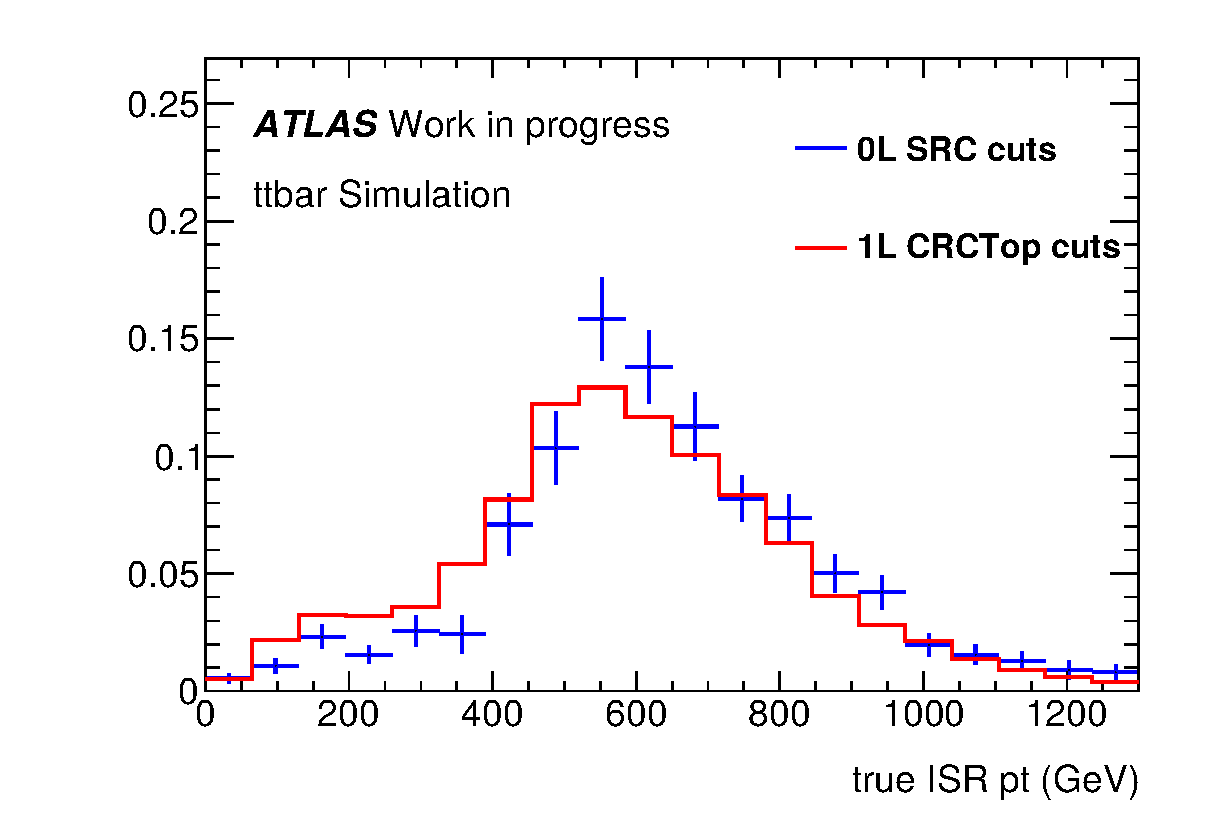
\includegraphics[width=0.65\textwidth]{./figures/ttbar/truePtISR_SRC_CRC_compare.eps}
\caption{\label{fig:ttbar:CR:trueISRpt}{Distribution of true ISR pt for ttbar that survive the CR and SR selections.  Both peak at roughly 550 $\gev$ demonstrating that the one lepton CR and zero lepton SR captures the same population of ttbar plus strong ISR.  Therefore, the one lepton CR essentially measures the amount of ttbar in SR directly from data with little extrapolation over ISR $\pt$.}}
\end{figure}

\indent In the one lepton CRCTop, the lepton is included as a ``jet'' in the Jigsaw ISR algorithm and will be counted as a sparticle jet or an ISR jet depending on which hemisphere it falls.  The lepton is meant to play the role of a hadronic tau jet in the zero lepton SR.  This approximation is justified since roughly 80 percent of all ttbar events in SR decay via the hadronic tau channel.  \\

\indent  Stop signal, especially those with $\Delta m \neq m_{t}$, tend to produce more $\met$ because of the presence of neutralinos.  A cut of $\mtlepmet < 80\gev$ is added to remove signal contamination.  
A $\mindrblep<2.0$ cut is added to increase ttbar purity and ensure orthogonality to the W+jets control region. \\

\indent The $\pTjV>50\gev$ cut is relaxed to $\pTjV>40\gev$ in order to increase statistics in the CR.  The $\pTjV$ cut specifies the $\pt$ of the 4th jet in the sparticle system.  The $\pTjV$ cut can be correlated with ISR/FSR because there is a chance that the 4th most energetic jet in the sparticle system is from radiation and not from a top decay.  However for this analysis it is more important to accurately gauge the amount of hard ISR of order hundred or more GeV that the ttbar system recoils against then amount of additional radiation in the same hemisphere as $\ttbar$. We found that loosening $\pTjV$ cut to 40 GeV does not result in a large difference in the true ISR pt distribution in the CRCTop and SR. \\

\subsubsection*{CRCTop Signal Contamination}

\indent Signal contamination in CRCTop ranges from 1 percent at high stop masses to 12 percent at low stop masses for all mass points not already excluded by previous stop experiments.  The largest signal contamination occurs at a stop mass of 225 to 250 $\gev$.   Here, the signal contamination approaches 12 percent due to the large stop production cross-section.  Lower stop masses result in higher signal contamination but our search does not have sensitivity to regions below 225 $\gev$.  \\

\indent The fact that CRCTop can attain such low signal contamination while selecting for ttbar background with such similar kinematic features as SR is impressive.  The SR has a signal to background ratio of approximately 2 to 1 for stop masses between 250 $\gev$ and 400 $\gev$.   In comparison, CRCTop is able to achieve SR contamination of around 5 to 12 percent for the same signal points.  \\

\indent CRCTop is able to make up for this factor of 20-40 difference in S/B rate mainly due to two reasons.  First CRCTop is a one lepton control region.  Working in the one lepton region means both signal and ttbar background draw from the single muon and single electron decay channels.  Signal and background therefore has similar decay fractions in CRCTop. The SR, on the other hand, mainly selects for signal with two tops that decay fully hadronically with roughly a 44 percent branching fraction.  In comparison, the ttbar background in SR main decay via the single hadronic tau decay channel with only a 10 percent decay fraction.  The CR therefore has a factor of 5 decrease in S/B ratio compared to the SR based on branching fraction alone.  \\

\indent The SR also gains S/B by enforcing the correlations between the ISR system and $\met$.  Removing the $\dphiISRI > 3.0$ requirements decreases S/B by another factor of 3. Including all regions of $\RISR$ in CRCTop and specifically targeting the $\RISR$ window under the signal peak decreases the S/B of 2 to 5 to the S/B depending on the stop mass and location of signal $\RISR$ peak.  Removing the requirement on these correlations do no change the requirement on strong ttbar ISR $\pt$ but opens up more phase space for ttbar to decay.  \\

\indent The two factors combine to make up the roughly factor of 30 decrease in S/B between SR and CRCTop; all the while preserving the agreement in true ttbar ISR $\pt$ distribution shown in figure \ref{fig:ttbar:CR:trueISRpt}. \\

\subsubsection*{CRCTop Distributions}

\indent Distribution of important variables after normalization to $\intlumi$ $\ifb$ of data are shown for CRCTop in figure \ref{fig:CRTopC}.  There seem to be no significant slope in the data over MC comparison in the CRCTop $\pTjV$ distribution.  This is further evidence that the extrapolation from 40 to 50 GeV across $\pTjV$ is allowed.  \\

\indent There is a noticeable trend in the data over MC comparison in the CRCTop $\pTISR$ distribution.  The disagreement is not surprising given that a priori we have an 30 percent uncertainty due to the ISR/FSR uncertainty.  This further demonstrate the need for a CR that directly measures the amount of ttbar with strong ISR pt in data. \\

\begin{figure}[htbp]
  \begin{center}
    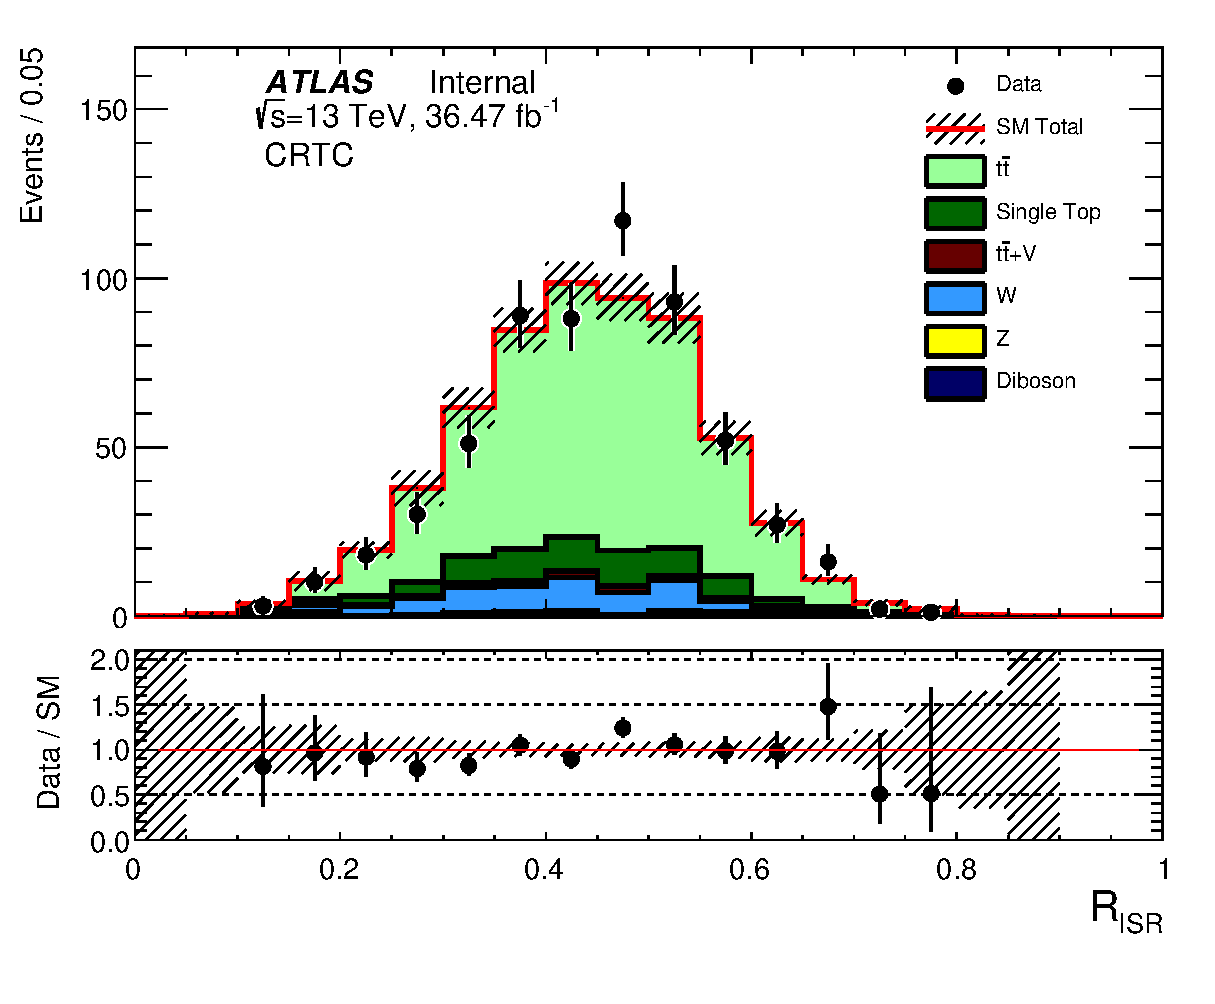
\includegraphics[width=0.45\textwidth]{figures/ttbar/postfit/CA_RISR_CRTopC}
    \includegraphics[width=0.45\textwidth]{figures/ttbar/postfit/CA_pTISR_CRTopC}
    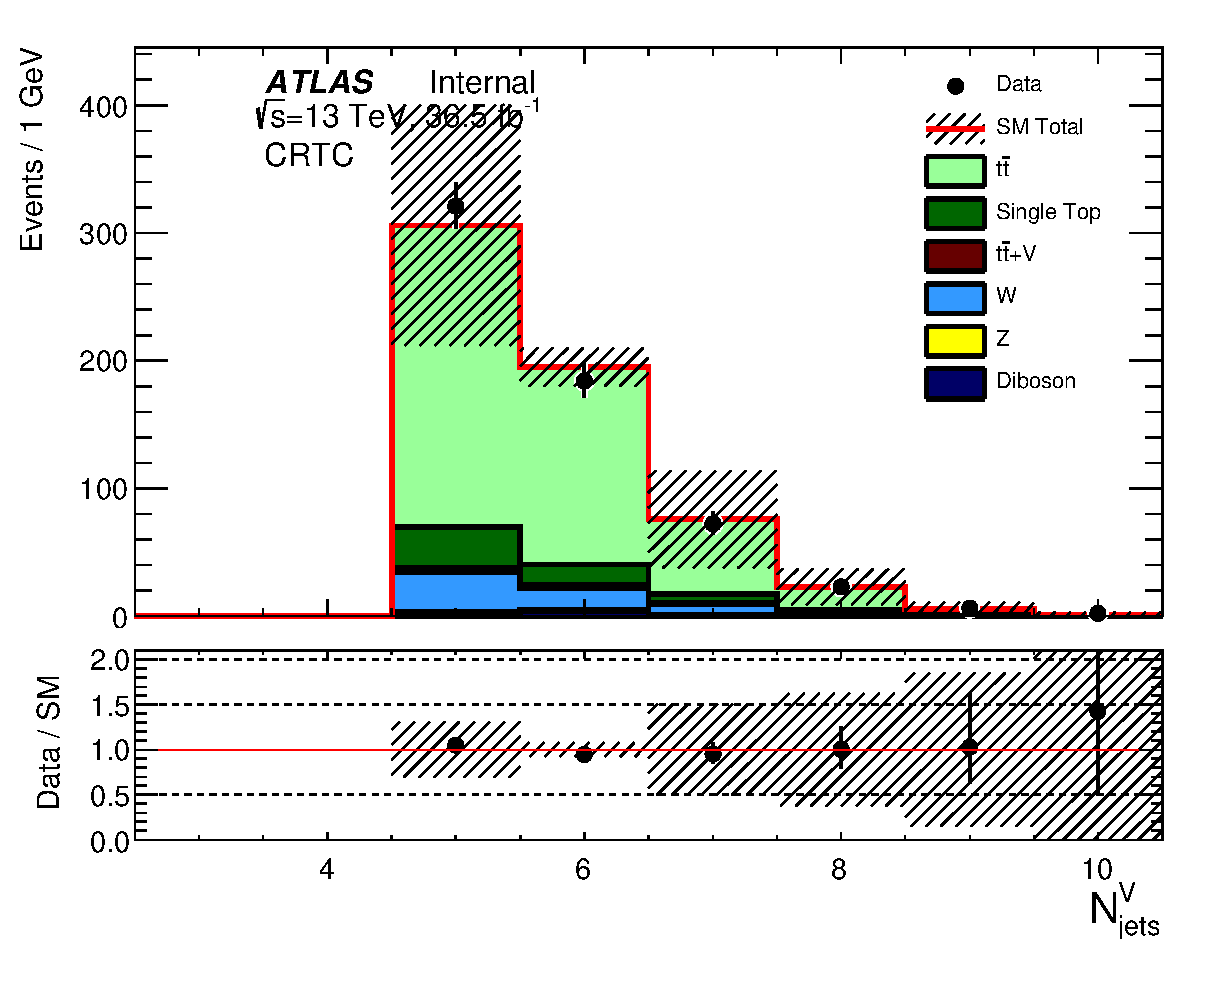
\includegraphics[width=0.45\textwidth]{figures/ttbar/postfit/CA_NjV_CRTopC}
    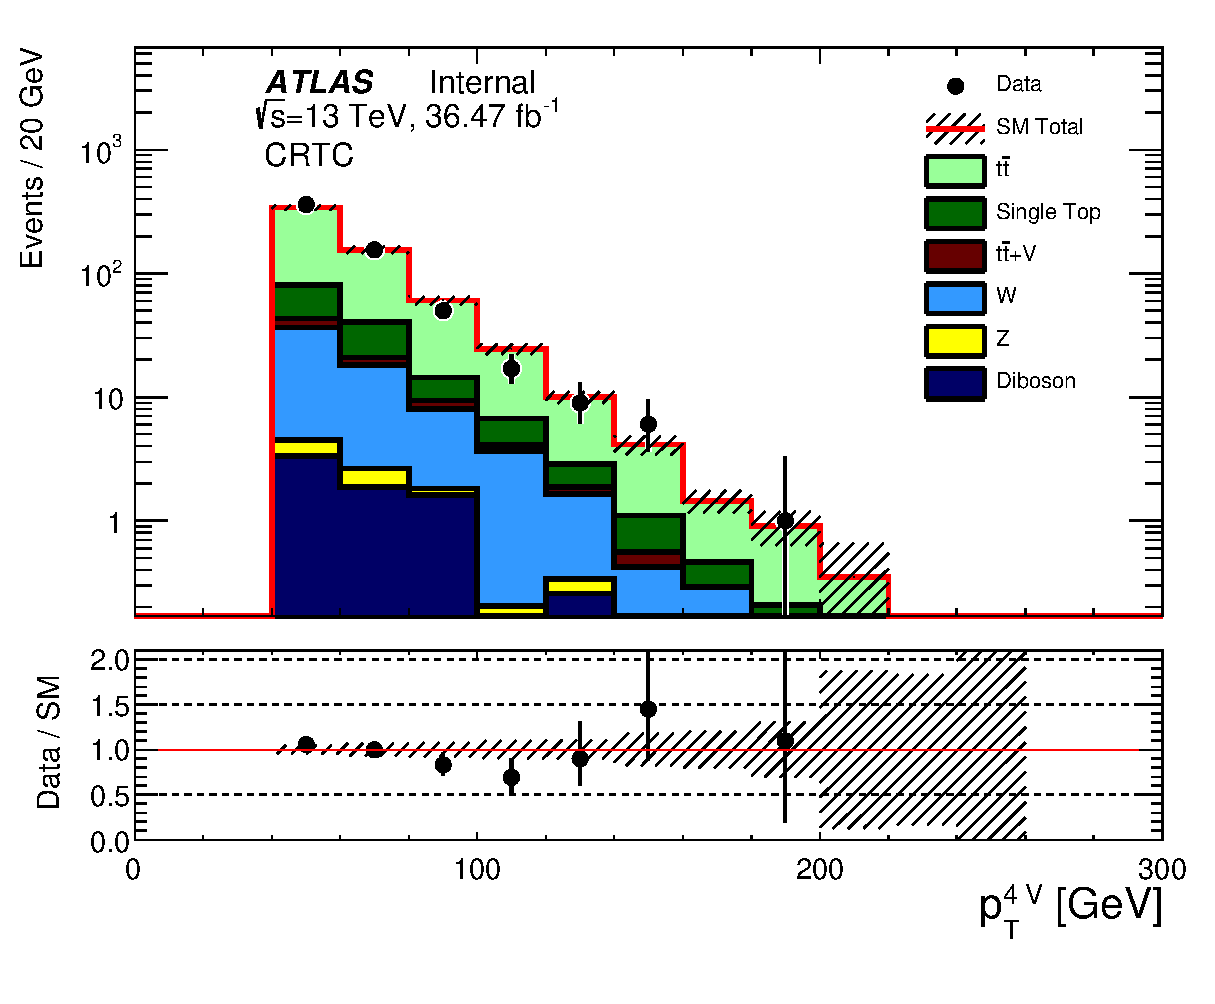
\includegraphics[width=0.45\textwidth]{figures/ttbar/postfit/CA_pTjV4_CRTopC_log}
    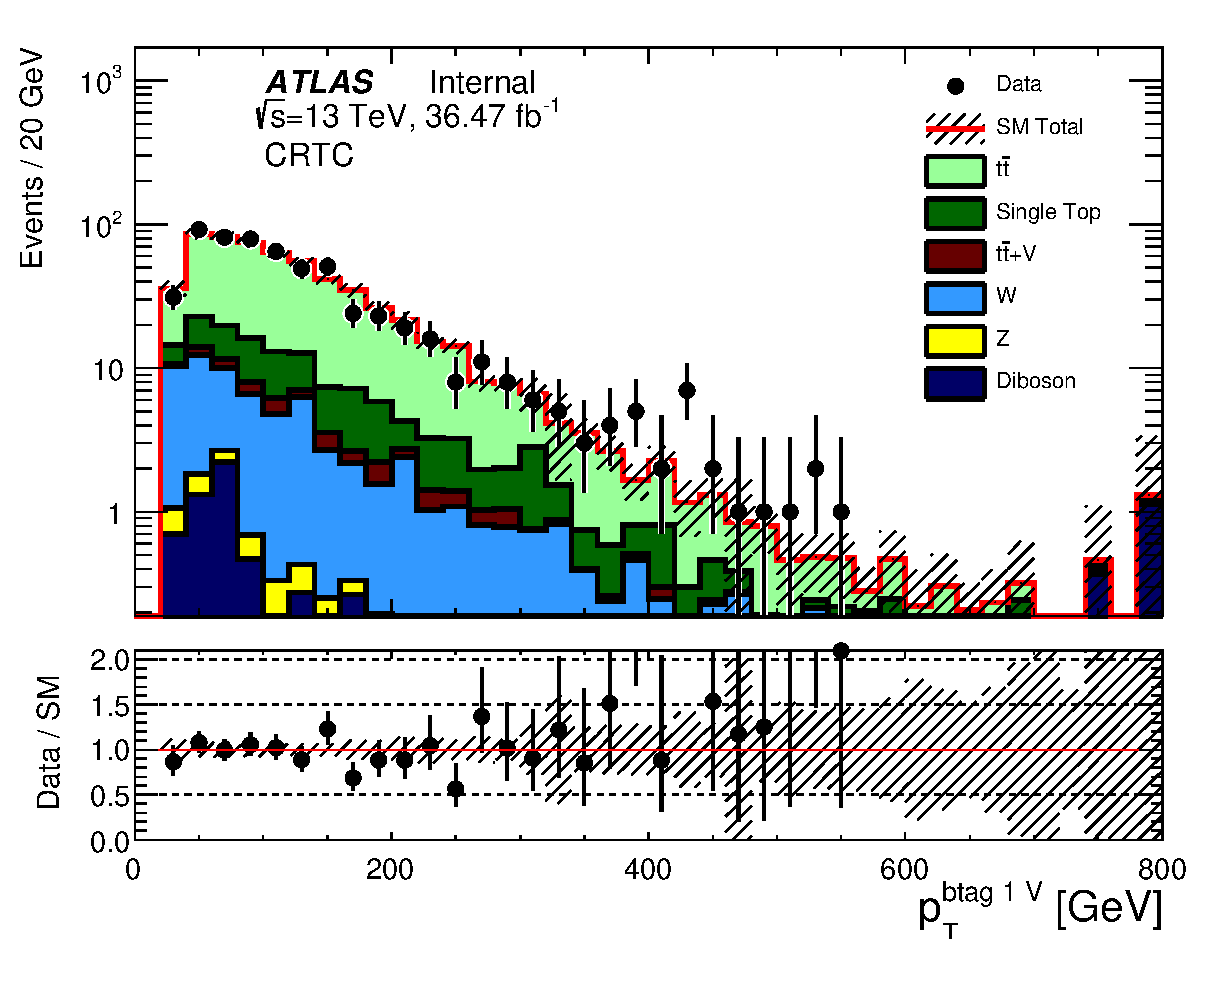
\includegraphics[width=0.45\textwidth]{figures/ttbar/postfit/CA_pTbV1_CRTopC_log}
        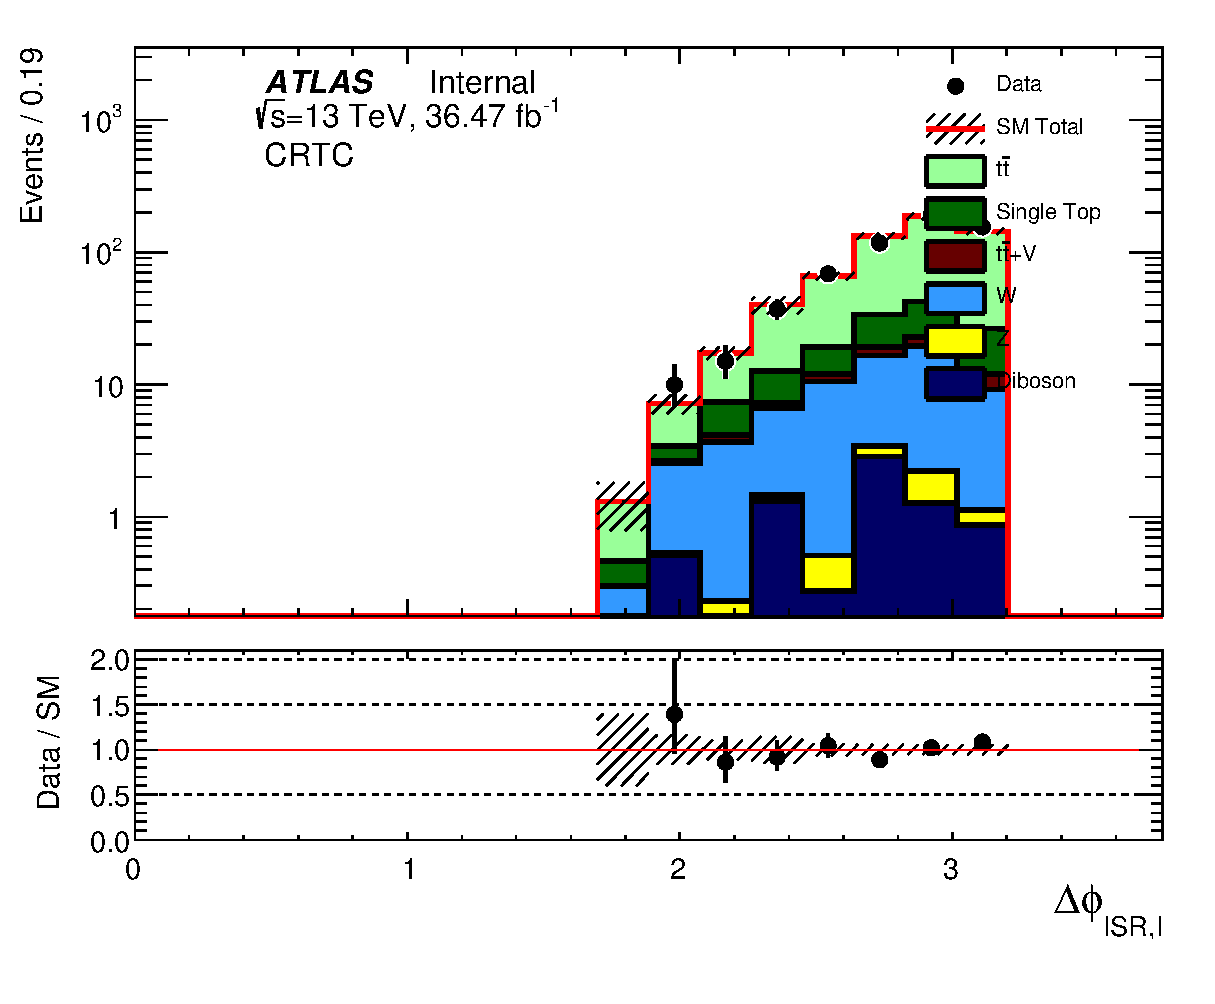
\includegraphics[width=0.45\textwidth]{figures/ttbar/postfit/CA_dphiISRI_CRTopC_log}
  \end{center}
  \caption{One lepton ttbar CR (CRCTop) distributions for $\intlumi$ $\ifb$ of data. All backgrounds have already been normalized to CRs by performing a background only fit.  The ratio between data and MC is shown in the bottom panel. The hashed area in both the top and lower panel represent the uncertainty due to MC statistics and detector systematic uncertainties.}
  \label{fig:CRTopC}
\end{figure}

\indent The normalization scale factor for ttbar is 0.707 according to a background only fit on $\intlumi$ $\ifb$ of data. This scale factor is quiet different from 1.0 which indicates that the ttbar MC alone does not well model the high ISR $\pt$ phase space.  Again, this difference is not unexpected given the 30 percent ISR/FSR uncertainty on ttbar MC.  \\

\subsection{Validating $\ttbar$ Predictions in Signal Region using a Zero Lepton Validation Region}
\label{sec:Bkg:ttbar:VR}

\indent We also define a zero lepton ttbar VR to validate the predicted background rates in SR.  The ttbar VR (VRCTop) is kinematically similar to SR but has the $\dphiISRI < 3.0$ selection is inverted to ensure orthogonality and limit signal contamination. In ttbar events, $\dphiISRI$ specifies the direction of neutrino relative to the direction of the ISR.  Inverting the $\dphiISRI$ selection only selects for ttbar with a different decay axis but does not change the requirements on strong ISR $\pt$.  The $\dphiISRI < 3.0$ selection does effectively reject stop events because the neutralinos gain all their momenta from the ISR system in signal. \\

\indent The requirement on $\MS$ is reduced to 100 GeV (vs. 300 GeV in the SR) and an $\NjV \ge 4$ selection is applied (vs. $\NjV \ge 5$ in the SR) to enhance the yields of semi-leptonic $\ttbar$ events . A requirement of $\MV/\MS < 0.6$ is added to reduce signal contamination and reject QCD multijet background. \\

\indent Similar to CRCTop, the $\pTjV>50\gev$ selection is relaxed to $\pTjV>40\gev$ to increase VR statistics. \\

\begin{table}
  \caption{Zero-lepton \ttbar+ISR validation region definitions, in addition
    to the SRC requirements listed in Table~\ref{tab:SRcommon}.}
  \begin{center}
    \def\arraystretch{1.4}%
    \begin{tabular}{c||c} \hline\hline
      {\bf Variable} & \\ \hline \hline
      \NjV           & $\ge4$                \\
      \NbV           & $\ge1$                \\
      \pTbV          & $\ge 40$              \\
      \PTISR         & $\ge 400$             \\
      \MS            & $>100\gev$            \\
      $\MV/\MS$      & $<0.6$                \\
      \dphiISRI      & $<3.00$               \\ \hline \hline
    \end{tabular}
  \end{center}
  \label{tab:ttbar0LepVR}
\end{table}%

\indent The distributions of the selection variables in VRCTop are shown in Fig.~\ref{fig:ttbar0Lep1bVRISR}.  The background rates have been normalized to CRs through the use of a background only fit to $\intlumi$ $\ifb$ of data. \\

\begin{figure}[htbp]
  \centering
    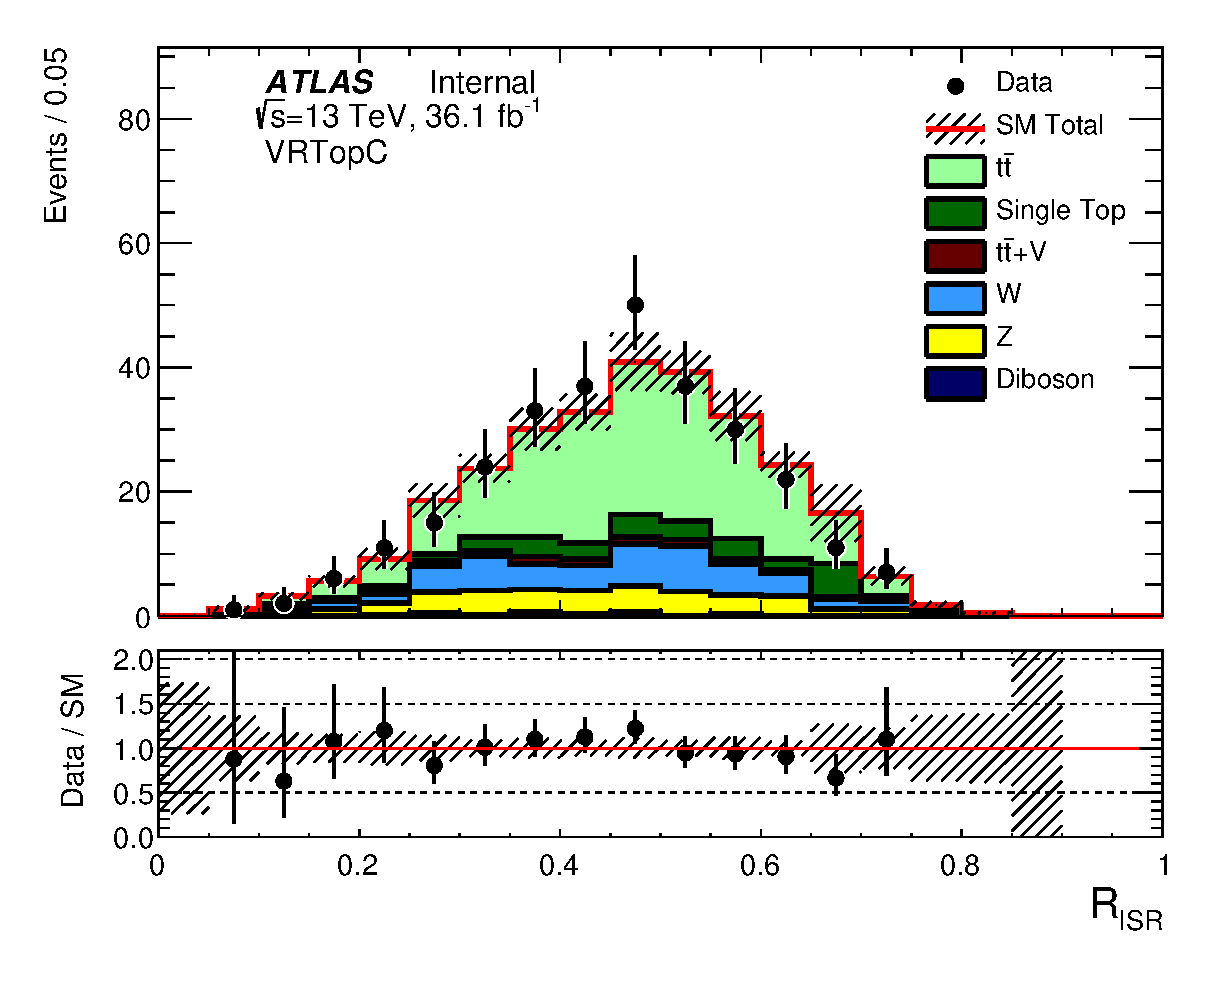
\includegraphics[width=0.45\textwidth]{figures/ttbar/postfit/CA_RISR_VRTopC}
    \includegraphics[width=0.45\textwidth]{figures/ttbar/postfit/CA_pTISR_VRTopC}
    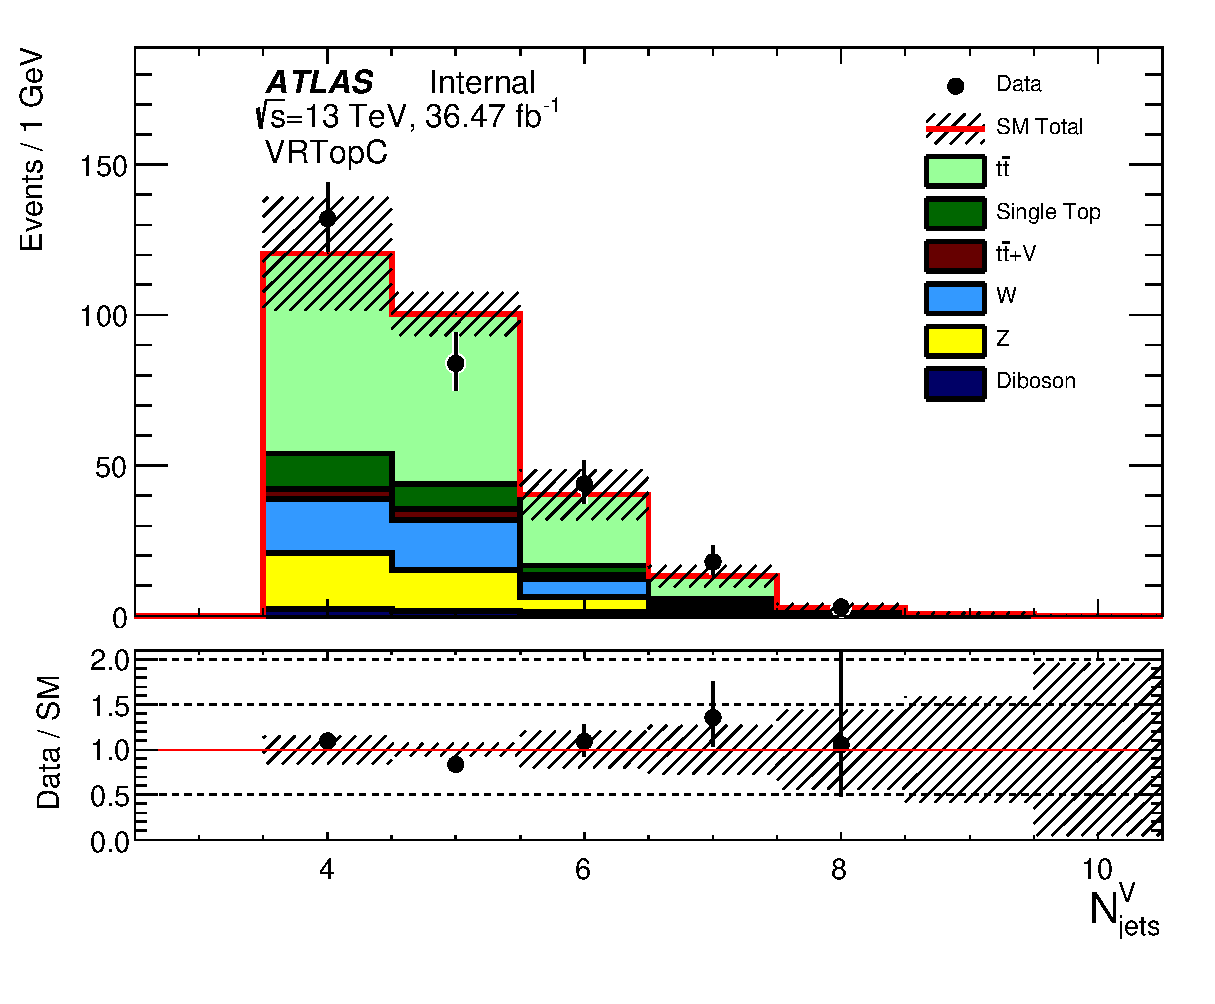
\includegraphics[width=0.45\textwidth]{figures/ttbar/postfit/CA_NjV_VRTopC}
    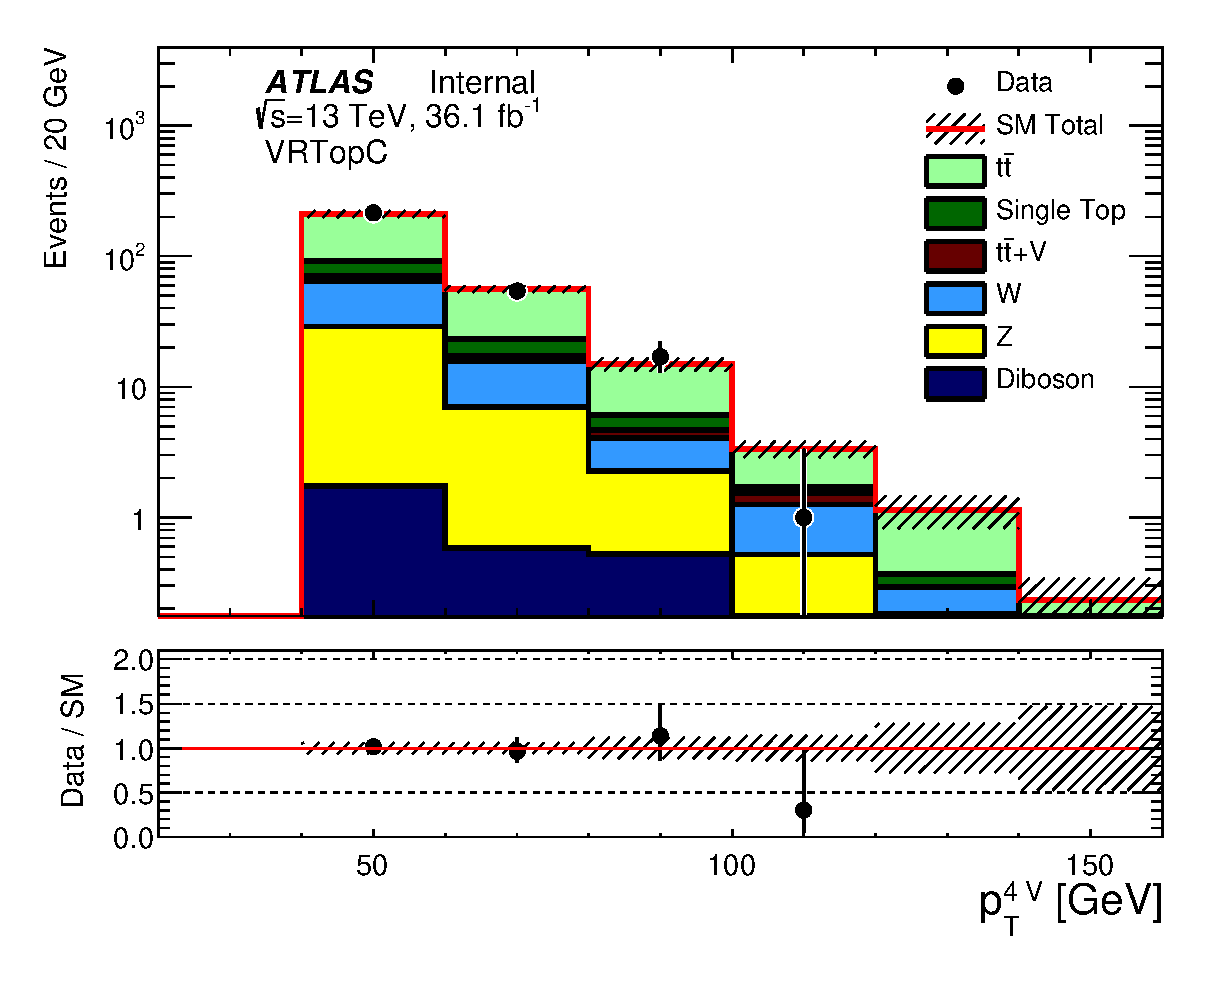
\includegraphics[width=0.45\textwidth]{figures/ttbar/postfit/CA_pTjV4_VRTopC_log}
    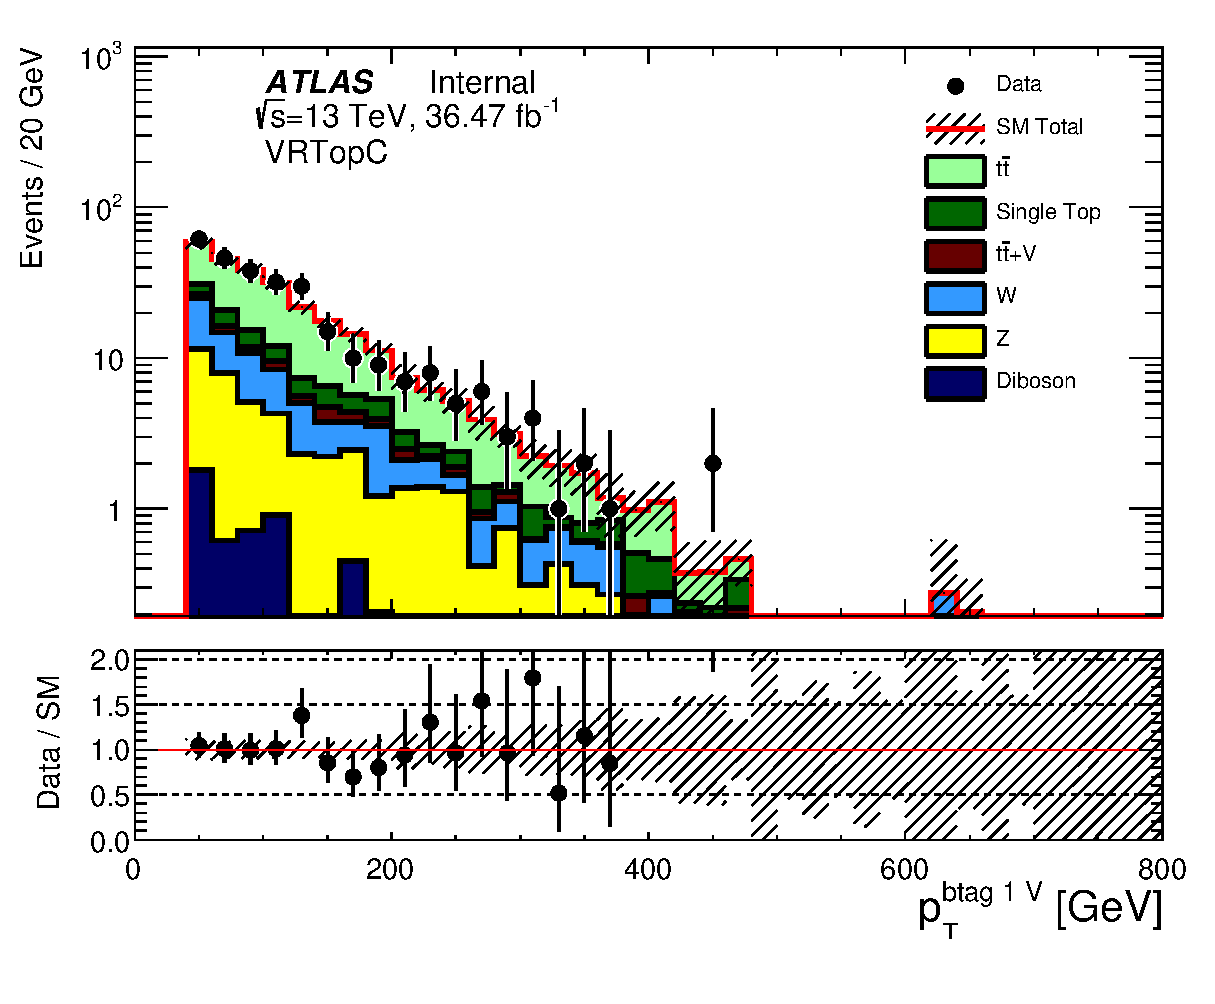
\includegraphics[width=0.45\textwidth]{figures/ttbar/postfit/CA_pTbV1_VRTopC_log}
        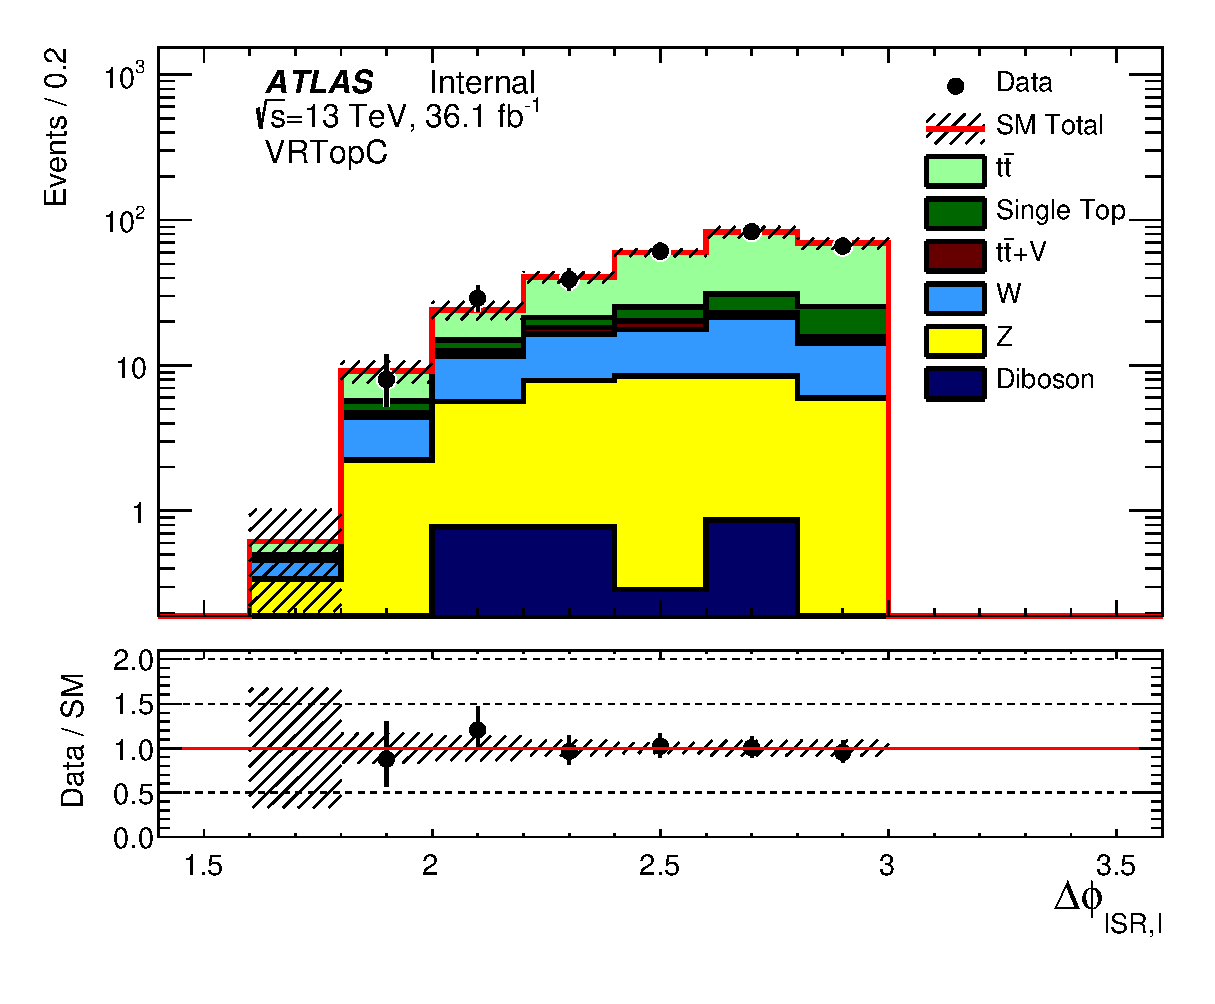
\includegraphics[width=0.45\textwidth]{figures/ttbar/postfit/CA_dphiISRI_VRTopC_log}
  \caption{\label{fig:ttbar0Lep1bVRISR}{Distribution of select variables in the zero lepton ttbar validation region.  The ratio between data and MC predictions are shown in the bottom panel.  The background rates have been normalized to CRs through the use of a background only fit to $\intlumi$ $\ifb$ of data.  Experimental systematic uncertainties on background predictions are depicted as the hashed bands. }}
\end{figure}

\indent The predicted background rate in the VRCTop agrees with data to within $1\sigma$.  This demonstrates that CRCTop is an effective predictor of ttbar background rates in VR and SR.  The $\RISR$ shape is well modeled as we see no distinct trends in the data vs MC ratio in $\RISR$. \\

\indent Similar to CRCTop, there is a noticeable trend in the data over MC comparison in the VRCTop $\pTISR$ distribution.  Again this is expected because the MC is a poor predictor of ISR $\pt$ rates.  The fact that data in VRCTop agrees with the predicted background rate proves that CRCTop can effectively measure the amount of ttbar with at least 400 $\gev$ of ISR $\pt$.  \\

%\indent This agreement both in magnitude and shape demonstrates two things.  One, the ttbar control region indeed does correctly measure the amount of ttbar plus strong ISR that exists in both signal and validation region.  Two, the sub-dominant background predictions also cannot by wrong by more than around 100 percent.  For example we clearly would see disagreement in between data vs MC in this VR if the MC underestimated W+jets or Z+jets background by 100 percent.  Both of these facts gives us confidence that the predictions for the amount of background in the signal region is correct. \\

\section{Subdominant Backgrounds}
\label{sec:Bkg:sub}

\subsection{Standard Model W+Jets}
\label{sec:Bkg:wjet}

\indent W boson produced in conjunction with QCD jets ($W$+jets) consists our largest sub-dominate background.  $W$+jets consists of 5 percent of the total background in the SR.  However the distribution of $W$+jets is not uniform across $\RISR$.  $W$+jets can reach around 15 percent of all background in the SR bins with the largest $\RISR$.  This means the $W$+jets contribution mostly affects the signal with high stop masses because those signal samples peak at high $\RISR$. \\

\indent We estimate $W$+Jets using a 1 lepton control region defined in section \ref{sec:WCR}.  The 1 lepton $W$+jet CR is orthogonal to the 1 lepton ttbar CR and 1 lepton single top CR defined in table \ref{tab:ttbar1LepCRISR_def} and \ref{tab:singleTop1LepCR_def} .  \\

\subsubsection{\Wjets\ Control Region}
\label{sec:WCR}

\indent The 1 lepton $W$+jet CR is designed to reject top events and ensure high $W$+jet purity.  The definition of the $W$+jets CR is given in table \ref{tab:WJetCR}. \\

\begin{table}[htpb]
  \caption{Summary of the selection for the 1-lepton, $W$+jets control regions.}
  \begin{center}
    \begin{tabular}{c|c}
      \hline \hline
                                      & CRW                \\ \hline
      Number of leptons             & 1                                          \\ \hline
      Number of jets (incl. lepton) & $\geq 4$                                     \\ \hline
      $\pt$ of jets (incl. lepton)  & (80,80,40,40) GeV                            \\ \hline
      \mindphijettwomet             & $> 0.4$                                      \\ \hline
      $\met$                        & $>250$ GeV                                   \\ \hline
      \mtlepmet                     & ($>30, <100$ GeV) \\ \hline
      Number of $b$-jets            & $=1$                            \\ \hline
      \mantikttwelvezero            & $<60\,$GeV         \\ \hline
      \mindrblep                    & $>2.0$             \\ \hline \hline
    \end{tabular}
  \end{center}
  \label{tab:WJetCR}
\end{table}

\indent The signal lepton is treated as a jet for the jet multiplicity and the jet $\pt$ requirement as well as for the top reconstruction.The mass requirement on the large R jet $\mantikttwelvezero < 60 \gev$ rejects events with reconstructed boosted tops.  The $\mtlepmet$ selection ensures that the transverse mass is consistent with those originating from a $W$ boson.  \\

\indent Orthogonality between $W$+jet CR and the single top CR is ensured by the requirement on the number of $b$-jets.  Orthogonality between ttbar CR and $W$+jet CR is ensured by the selection on $\Delta R(b_{0,1},\ell)_{\mathrm{min}}$, defined as the minimum $\Delta R$ between the two jets with the highest b-tag value and the selected lepton.  The signal contamination is less than 10\% for all signal points.  \\

\indent Data vs MC comparisons in the $\Wjets$ control region are shown in histograms in figure ~\ref{fig:CRWpts}.  The expected MC background has been normalized to the amount of data in the $\Wjets$ control region by performing a simultaneous fit to all background CR.  The hashed bands on the total SM background correspond to the amount of total experimental systematical uncertainty plus the MC statistical uncertainty.  The yield in the $\Wjets$ CR is given in table~\ref{tab:CRW_yields}.  \\

\indent  Data and MC are compatible to within statistical uncertainty.  No strong trends are observed in the data to MC ratios in any of the distribution. \\
\begin{table}[!htb]
  \centering
  \begin{tabular}{c|c}
\hline\hline
\multicolumn{2}{c}{\bf CRW (60\% purity)} \\ \hline 
Z & 1.99 $\pm$ 0.45 \\
dibosons & 9.85 $\pm$ 1.76 \\
ttbar & 128.42 $\pm$ 3.82 \\
singleTop & 51.14 $\pm$ 3.37 \\
ttV & 1.07 $\pm$ 0.16 \\
W & 288.12 $\pm$ 8.86 \\
\hline
Total MC & 480.58 $\pm$ 10.38 \\
Data & 531.00 $\pm$ 23.04 \\
 \hline
SF & 1.17 $\pm$ 0.10 \\
\hline\hline
\end{tabular}

  \caption{Yields in the $\Wjets$ CR with \intlumi\ \ifb\ of data.  }
  \label{tab:CRW_yields}
\end{table}

\begin{figure}[!htb]
  \centering
  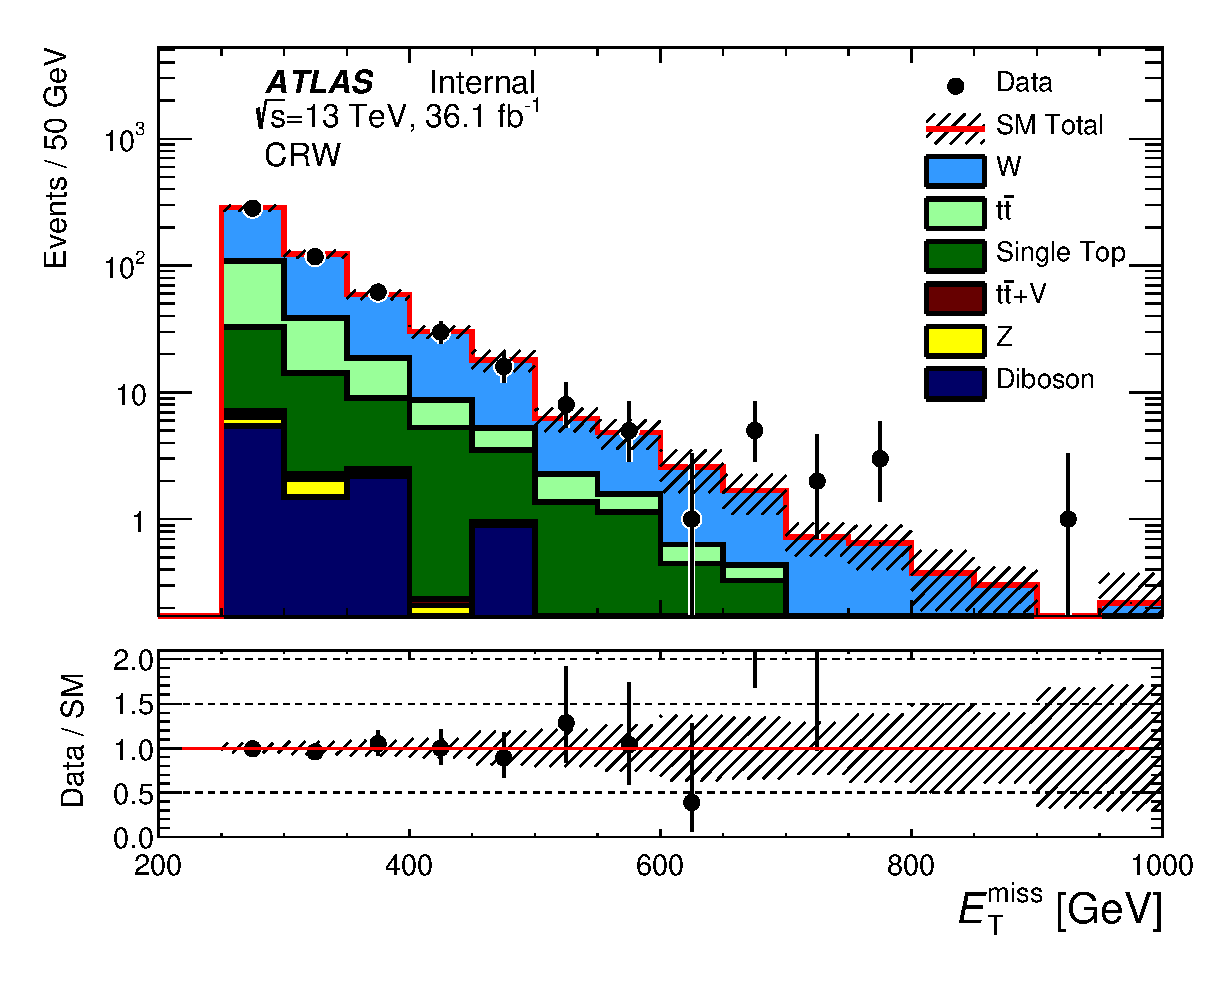
\includegraphics[width=0.45\textwidth]{figures/wJets/postfit/Met_CRW_log.eps}
    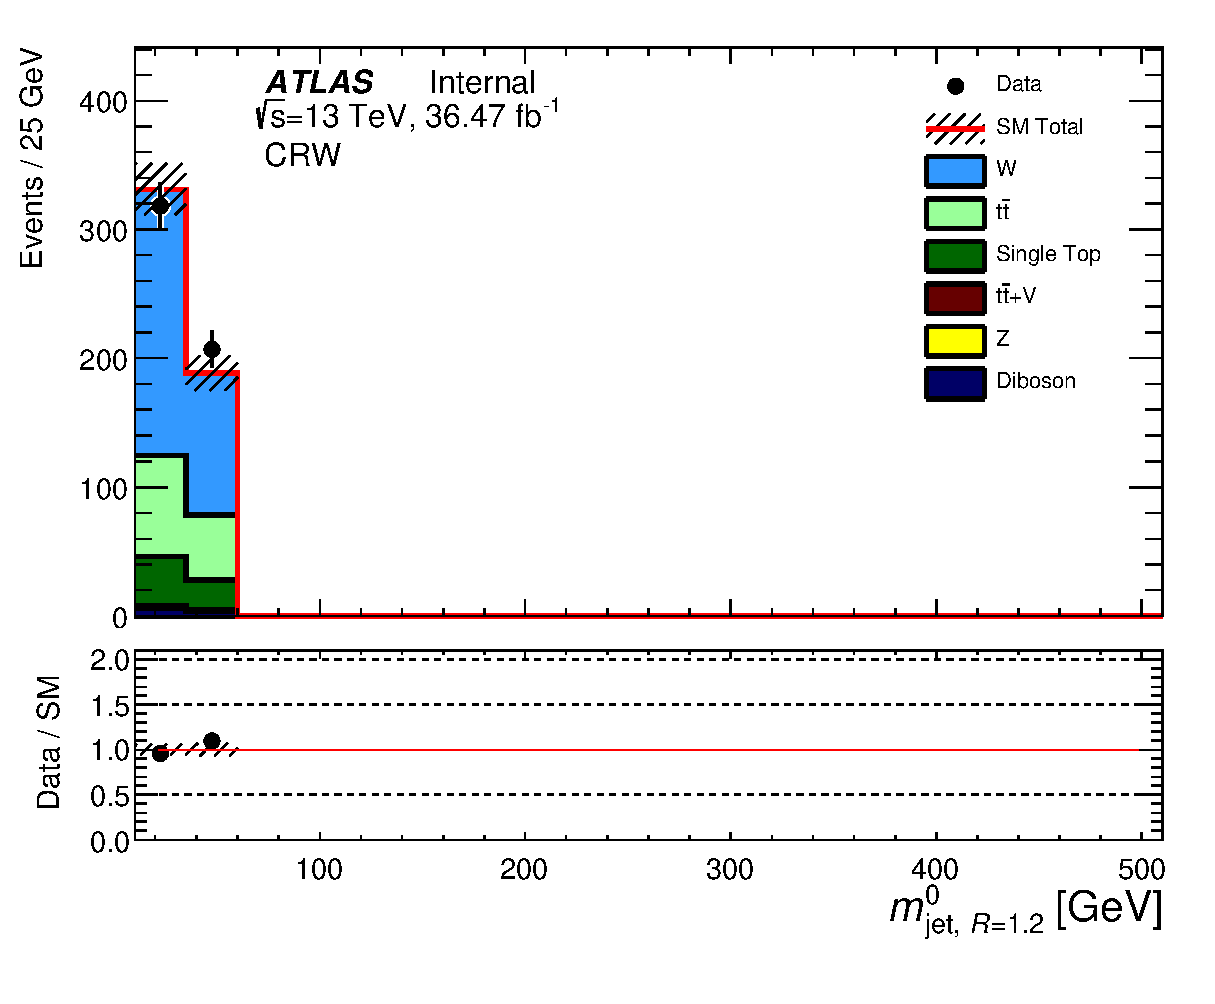
\includegraphics[width=0.45\textwidth]{figures/wJets/postfit/AntiKt12M_0__CRW.eps}
  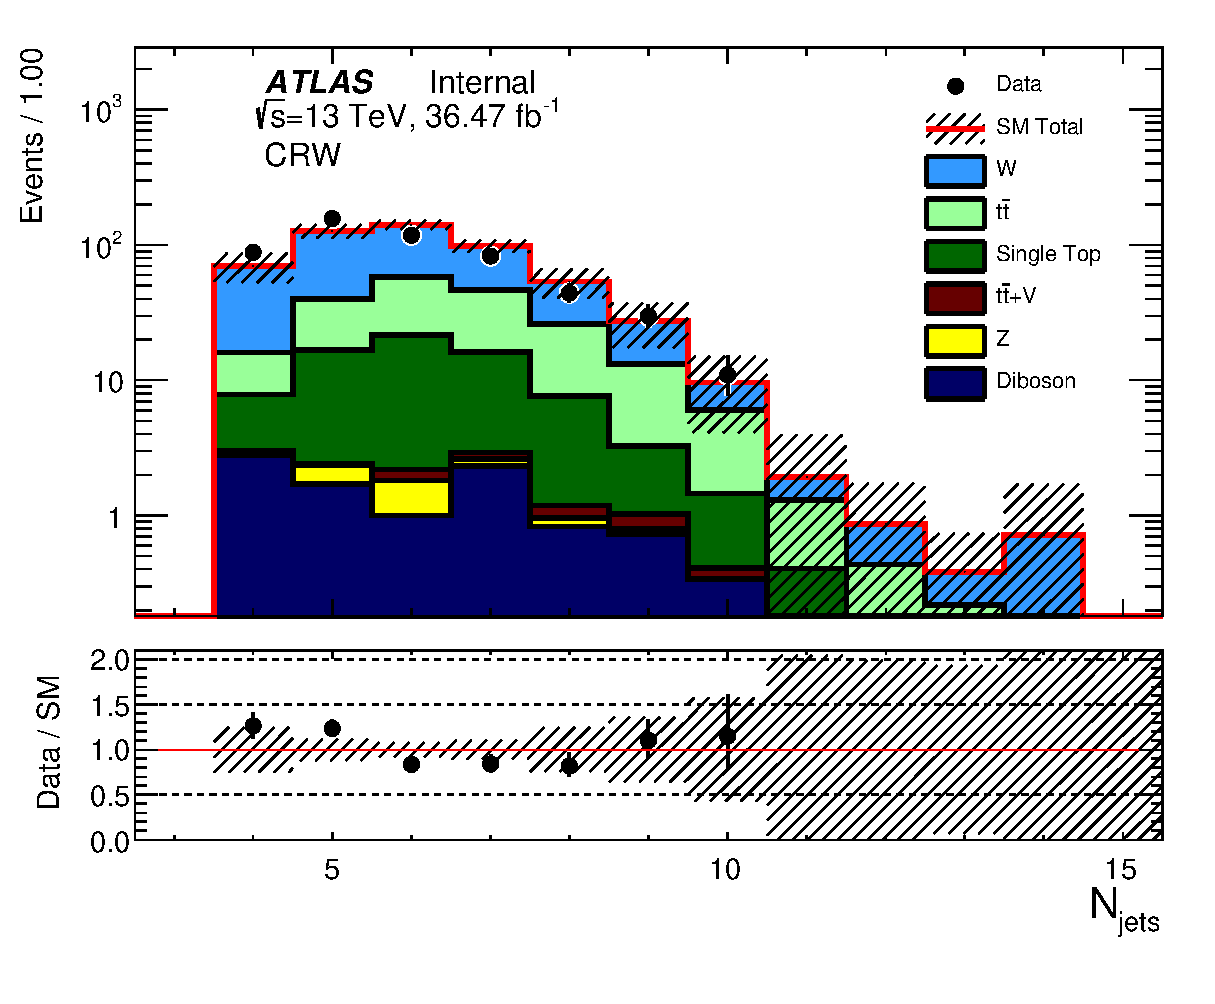
\includegraphics[width=0.45\textwidth]{figures/wJets/postfit/NJets_CRW_log.eps}
  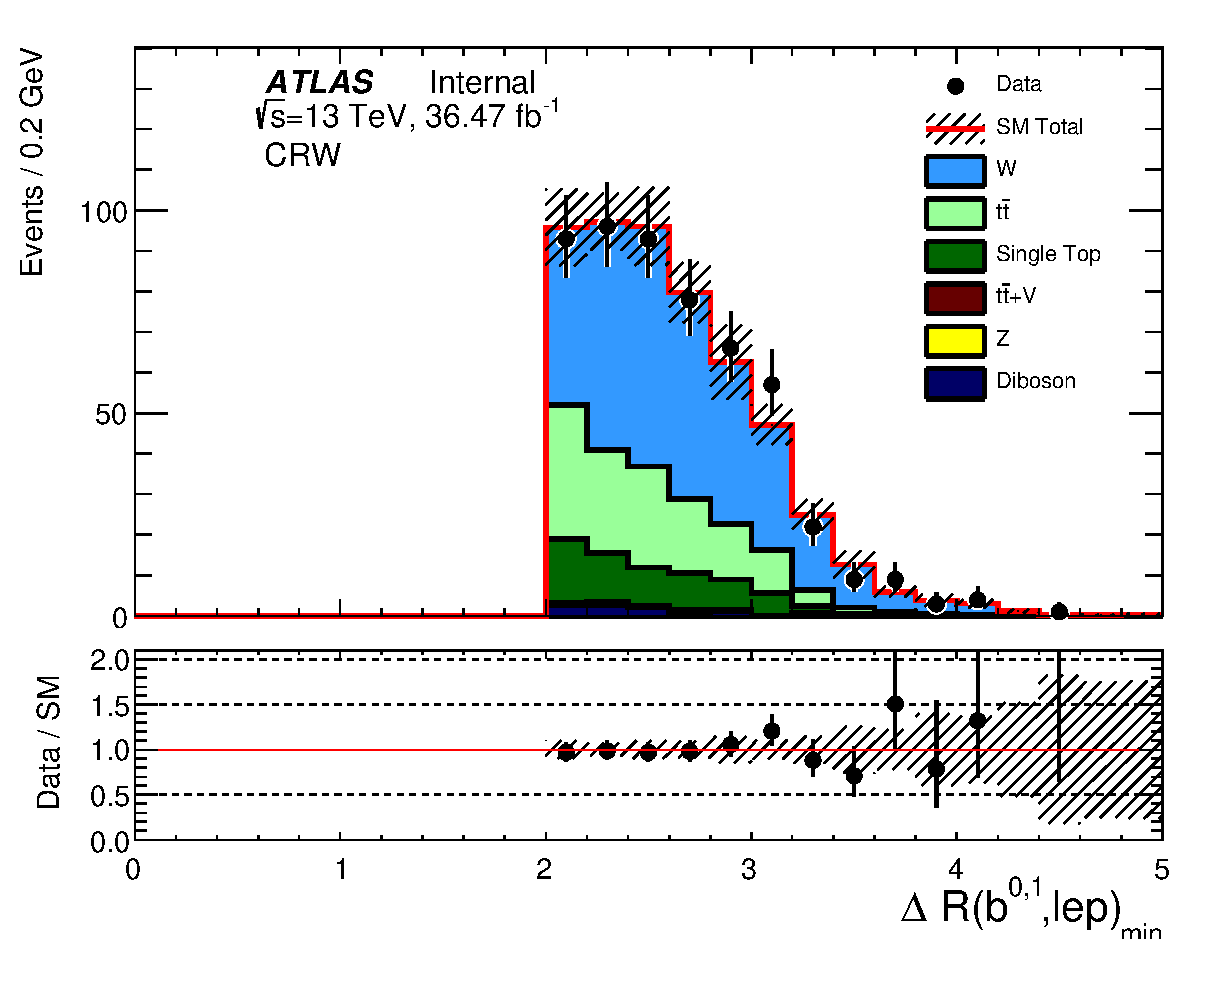
\includegraphics[width=0.45\textwidth]{figures/wJets/postfit/MinDRBLep_CRW.eps}]
  \caption{Postfit data/MC comparisons in the $\Wjets$ CR. From left to right and top to bottom, the variables shown are $\met$, $\mtlepmet$, $\mantikttwelvezero$ and $\mindrblep$. The expected SM background has been normalized to data in the CR by performing a simultaneous fit to all background CR.  The hatched band on the total SM background correspond to the total experimental systematic uncertainty plus the MC statistical uncertainty.}
  \label{fig:CRWpts}
\end{figure}



\subsection{Standard Model Single-Top}
\label{sec:Bkg:SingleTop}

\indent Standard Model single-top consists of 6\% of the total background in the signal region.  This rate varies between 2-9\% for any one signal region $\RISR$ bin.  A one-lepton single-top control region is defined in Table \ref{tab:ST1LCR}.  The single-top control region is orthogonal to both the one-lepton $W$+jets control region and $\ttbar$ control region.  \\

\begin{table}[h!]
  \caption{Selection for the one-lepton single-top control region.  The one-lepton preselection defined in Table \ref{tab:1Lcommon} is also applied.}
  \label{tab:ST1LCR}
  \begin{center}
    \begin{tabular}{c|c}
      \hline \hline
       { \bf Variables } & Single-top 1 lepton control region           \\ \hline
      Number of leptons             & 1                                            \\ 
      Number of jets (incl. lepton) & $\geq 4$                                     \\ 
      $\pt$ of jets (incl. lepton)  & (80,80,40,40) GeV                            \\ 
      \mindphijettwomet             & $> 0.4$                                      \\ \
      $\met$                        & $>250$ GeV                                   \\ \hline
      \mtlepmet                     & $>30$,$<100$ GeV \\ 
      Number of $b$-jets            & $\ge2$                          \\ 
      \mantikttwelvezero            & v$>120$ GeV       \\
      \mtbmin                       & $>200\,$GeV   \\ 
      \mindrblep                    & $>2.0$             \\ 
      \drbjetbjet                   & $>1.5$               \\ \hline \hline
    \end{tabular}
  \end{center}
\end{table}

\indent The lepton is treated as a jet for the jet multiplicity and the jet $\pt$ requirements as well as for the top reconstruction.  Similar to the one-lepton $\ttbar$ control region, the lepton is meant to play the role of a hadronic tau jet in the zero-lepton signal region. \\

\indent $\mtlepmet$ is defined in equation \ref{eqn:mtlep} as the transverse mass of the lepton and the $\met$.  The $\mtlepmet$ selection ensures that the transverse mass is consistent with a $W$ decay.  \\

\indent The $\drbjetbjet$ variable is defined in equation \ref{eqn:drbb} as the $\Delta R$ between the two b-jets with the highest b-tagging values.  $\drbjetbjet > 1.5$ isolates single-top events and rejects $\ttbar$.  This gives the single-top control region a purity of $\sim50\%$. \\

\begin{equation}
\mindrblep = \sqrt{ \Delta\eta(b_1, b_2)^2 + \Delta\phi(b_1, b_2)^2}
\label{eqn:drbb}
\end{equation}

\indent The $\mantikttwelvezero > 120 \gev$ requirement selects for events with reconstructed boosted tops and ensures orthogonality with the $\Wjets$ control region.  $\mantikttwelvezero$ is defined as the mass of an $\antikt$ jet built with a distance parameter of $R=1.2$ instead of the regular $R=0.4$.  The $\antikt$ algorithm clusters calorimeter energy into a jet according to the distance metric $R$ and is covered in detail in section \ref{sec:jet:reco}.  The large $R=1.2$ jet is designed to cluster all the energy of a boosted top quark into a single jet.  If the jet contains a boosted top, the invariant mass of jet should be close to $\sim m_t$.  \\

\indent $\mindrblep$ is defined in equation \ref{eqn:mindrblep} as the minimum $\Delta R$ between the two jets with the highest b-tag value and the selected lepton.  The $\mindrblep$ selection ensures orthogonality with the $\ttbar$ control region.  \\

\indent Kinematic distributions in the single control region are shown in Figure \ref{fig:CRST} and \ref{fig:CRST1}.  The MC background has been normalized to data by performing a simultaneous fit to all control regions.  The hashed bands on the total SM background correspond to the total experimental systematical uncertainty plus the MC statistical uncertainty.  The yield in the single-top control region is given in table~\ref{table.bkgonly.CRST}.  \\

\indent  Data and MC are compatible to within statistical uncertainty.  No strong trends are observed in the data to MC ratios in any of the distributions. \\

%\begin{table}[!htb]
%  \centering
%  \begin{tabular}{c|c}
\hline\hline
\multicolumn{2}{c}{\bf CRST (44\% purity)} \\ \hline 
Z & 0.11 $\pm$ 0.05 \\
dibosons & 1.52 $\pm$ 0.54 \\
ttbar & 34.17 $\pm$ 2.10 \\
singleTop & 45.62 $\pm$ 1.41 \\
ttV & 2.42 $\pm$ 0.19 \\
W & 19.72 $\pm$ 1.69 \\
\hline
Total MC & 103.57 $\pm$ 3.10 \\
Data & 113.00 $\pm$ 10.63 \\
 \hline
SF & 1.21 $\pm$ 0.29 \\
\hline\hline
\end{tabular}

%  \caption{Yields in the CRST in $\intlumi$ $\ifb$ of data.  }
%  \label{tab:CRST}
%\end{table}

\pagebreak
 
\begin{figure}[h!]
\begin{center}
      \begin{subfigure}[b]{0.40\textwidth}    
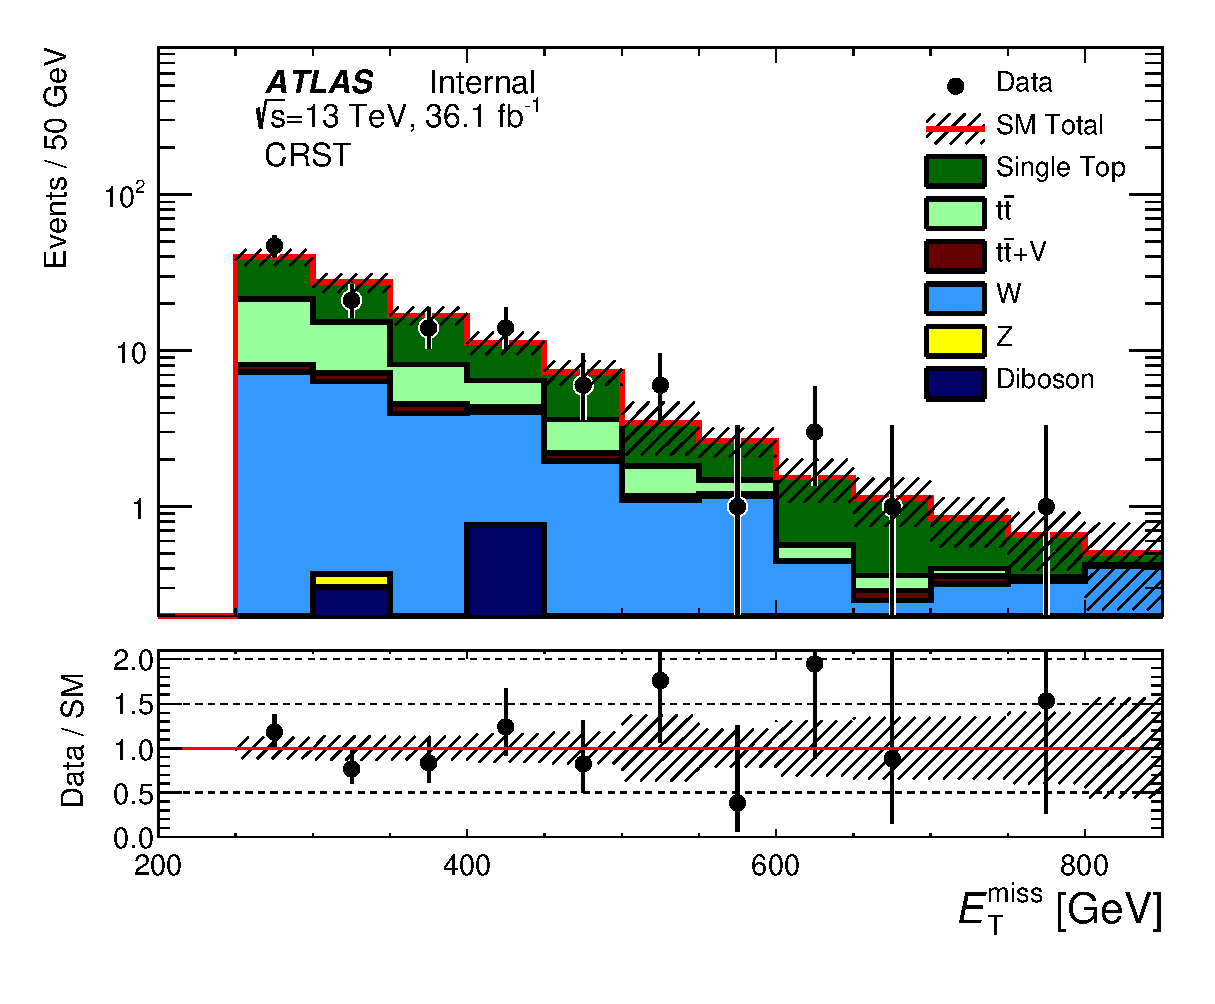
\includegraphics[width=\textwidth]{figures/singleTop/postfit/Met_CRST_log.eps}
                 \caption{ }
    \end{subfigure}
     \begin{subfigure}[b]{0.40\textwidth}    
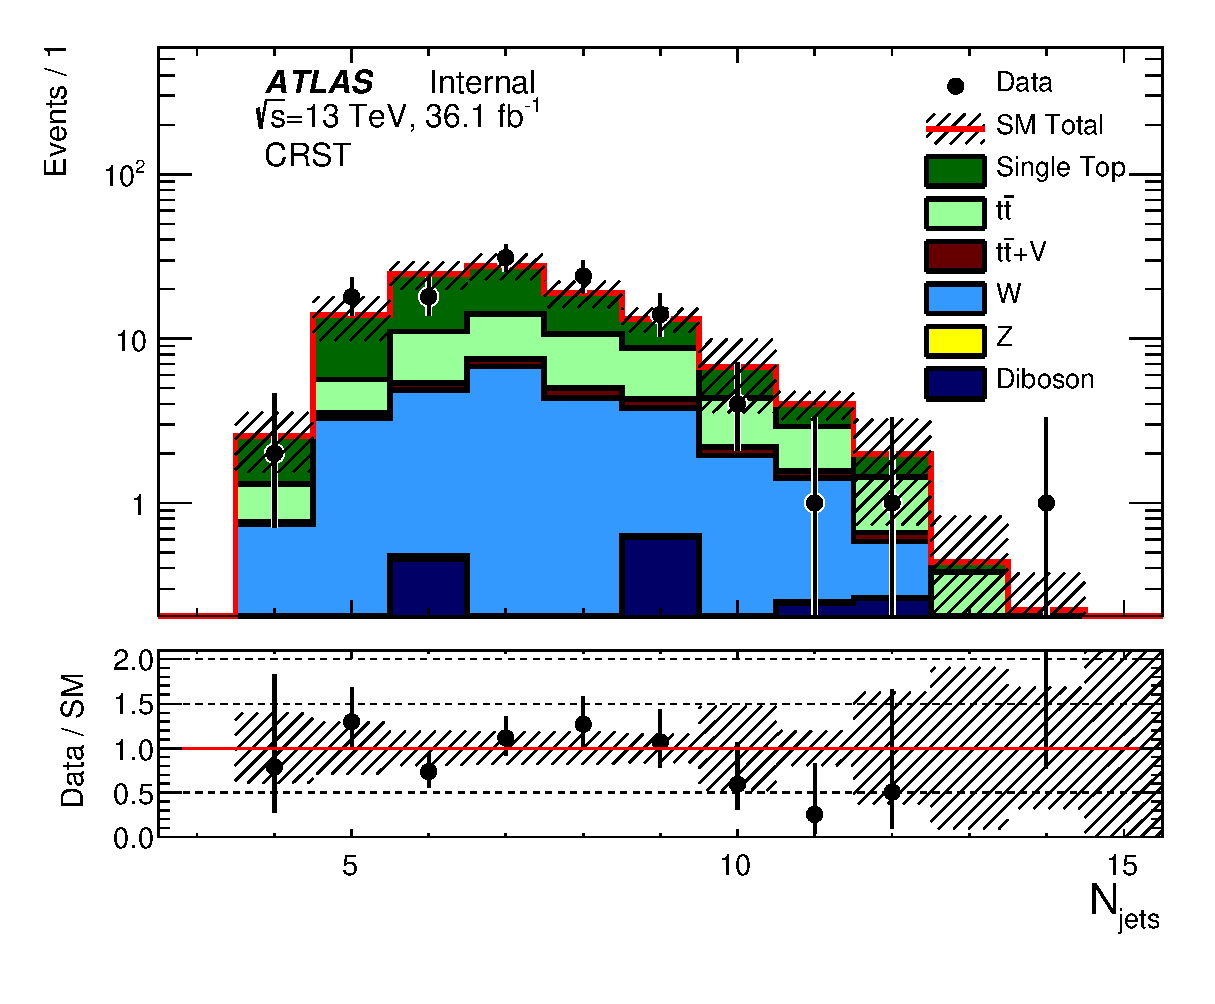
\includegraphics[width=\textwidth]{figures/singleTop/postfit/NJets_CRST_log.eps}
                \caption{ }
    \end{subfigure}
      \begin{subfigure}[b]{0.40\textwidth}    
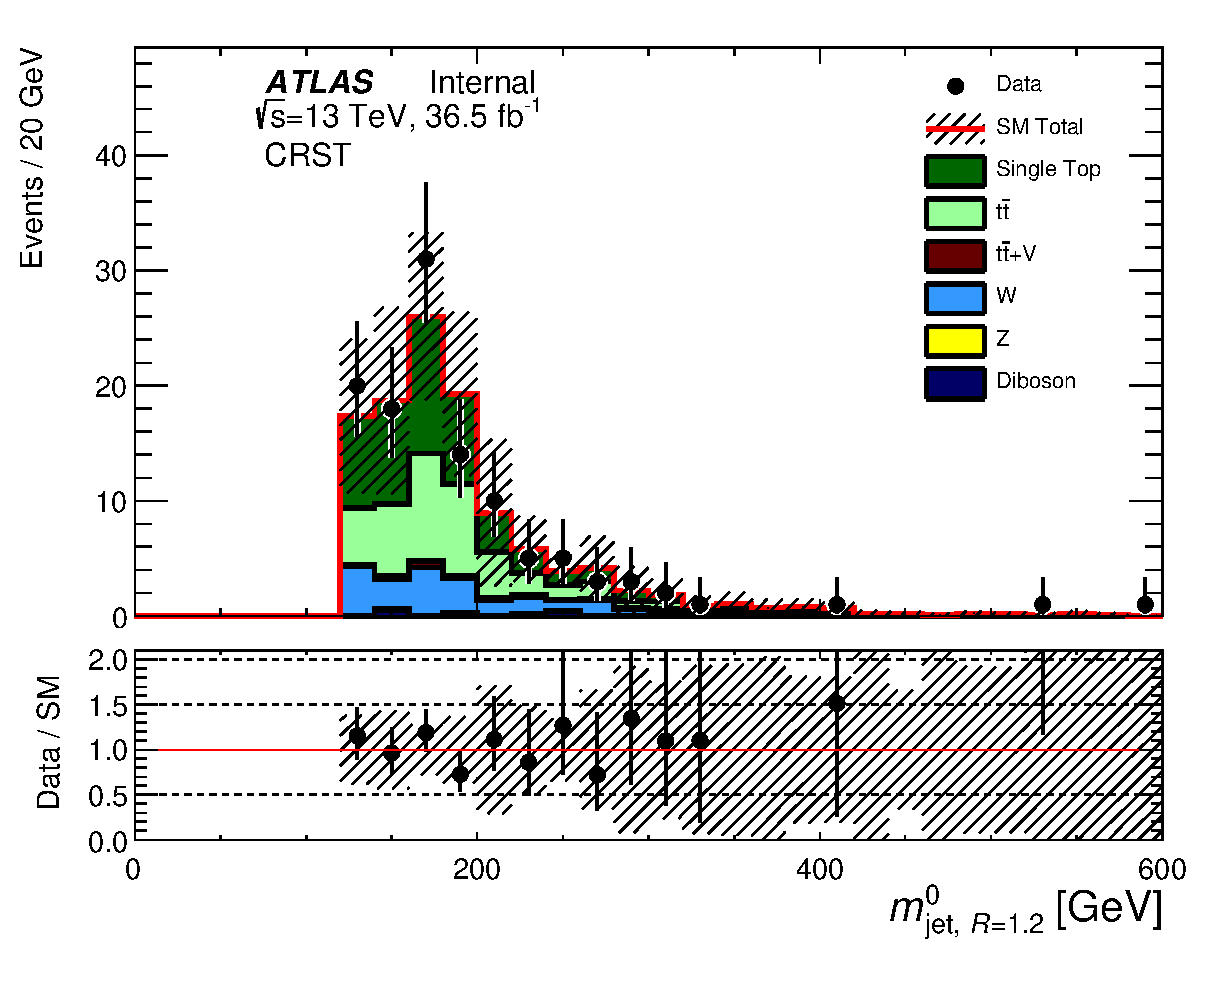
\includegraphics[width=\textwidth]{figures/singleTop/postfit/AntiKt12M_0__CRST.eps}
                \caption{ }
    \end{subfigure}
      \begin{subfigure}[b]{0.40\textwidth}    
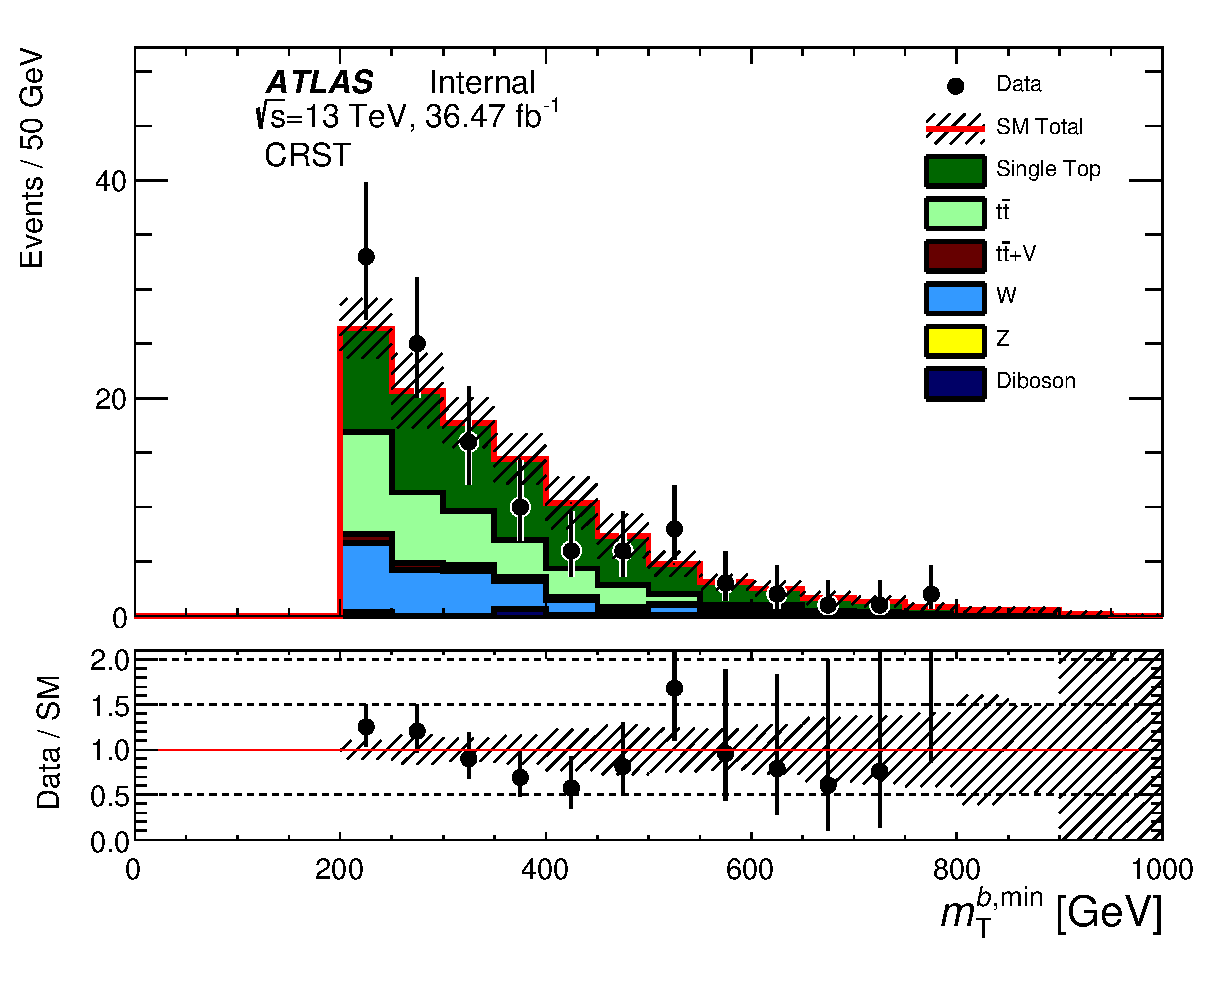
\includegraphics[width=\textwidth]{figures/singleTop/postfit/MtBMin_CRST.eps}
                \caption{ }
    \end{subfigure}
%      \begin{subfigure}[b]{0.40\textwidth}    
%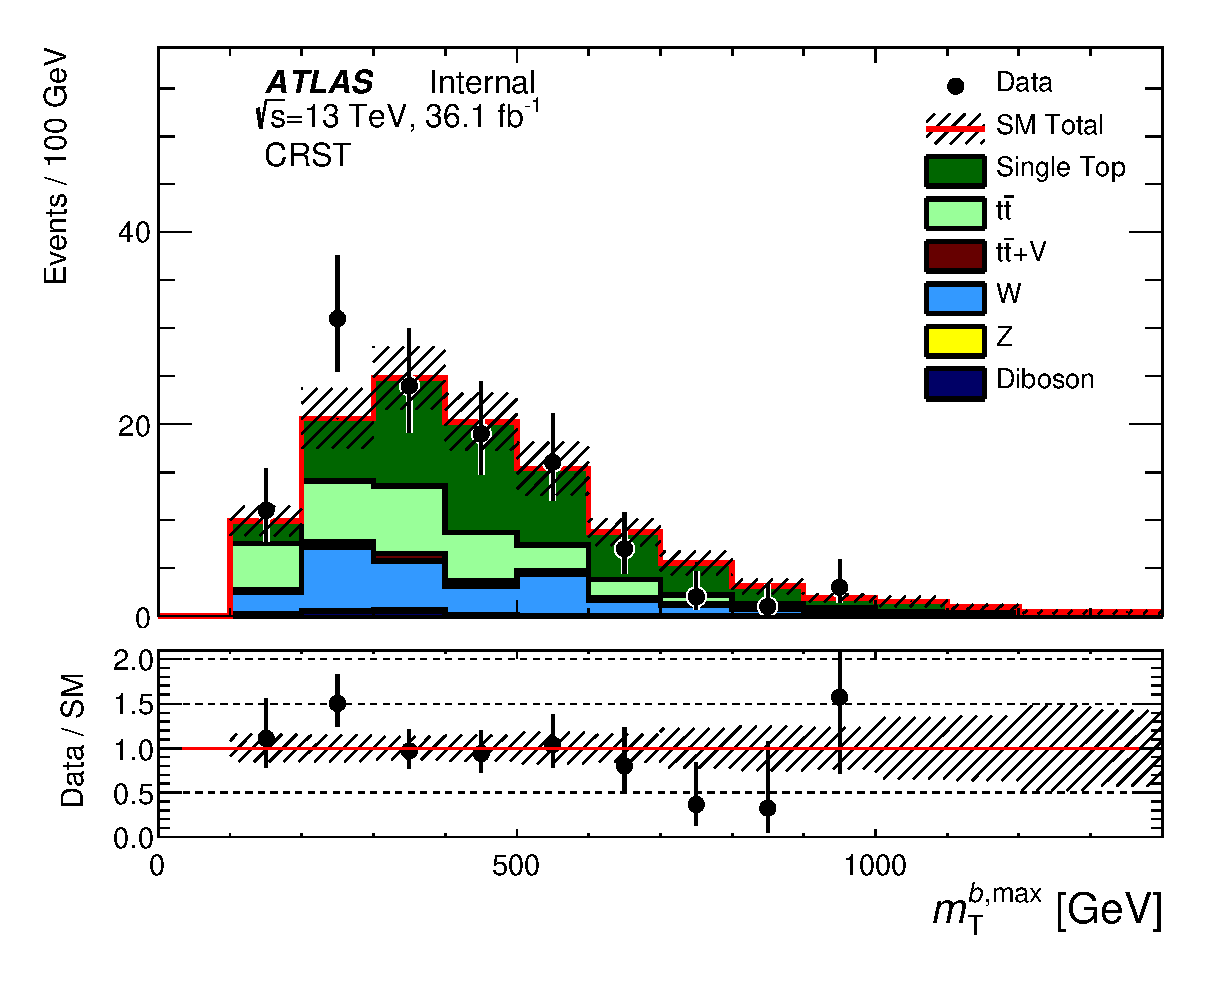
\includegraphics[width=\textwidth]{figures/singleTop/postfit/MtBMax_CRST.eps}
      \begin{subfigure}[b]{0.40\textwidth}    
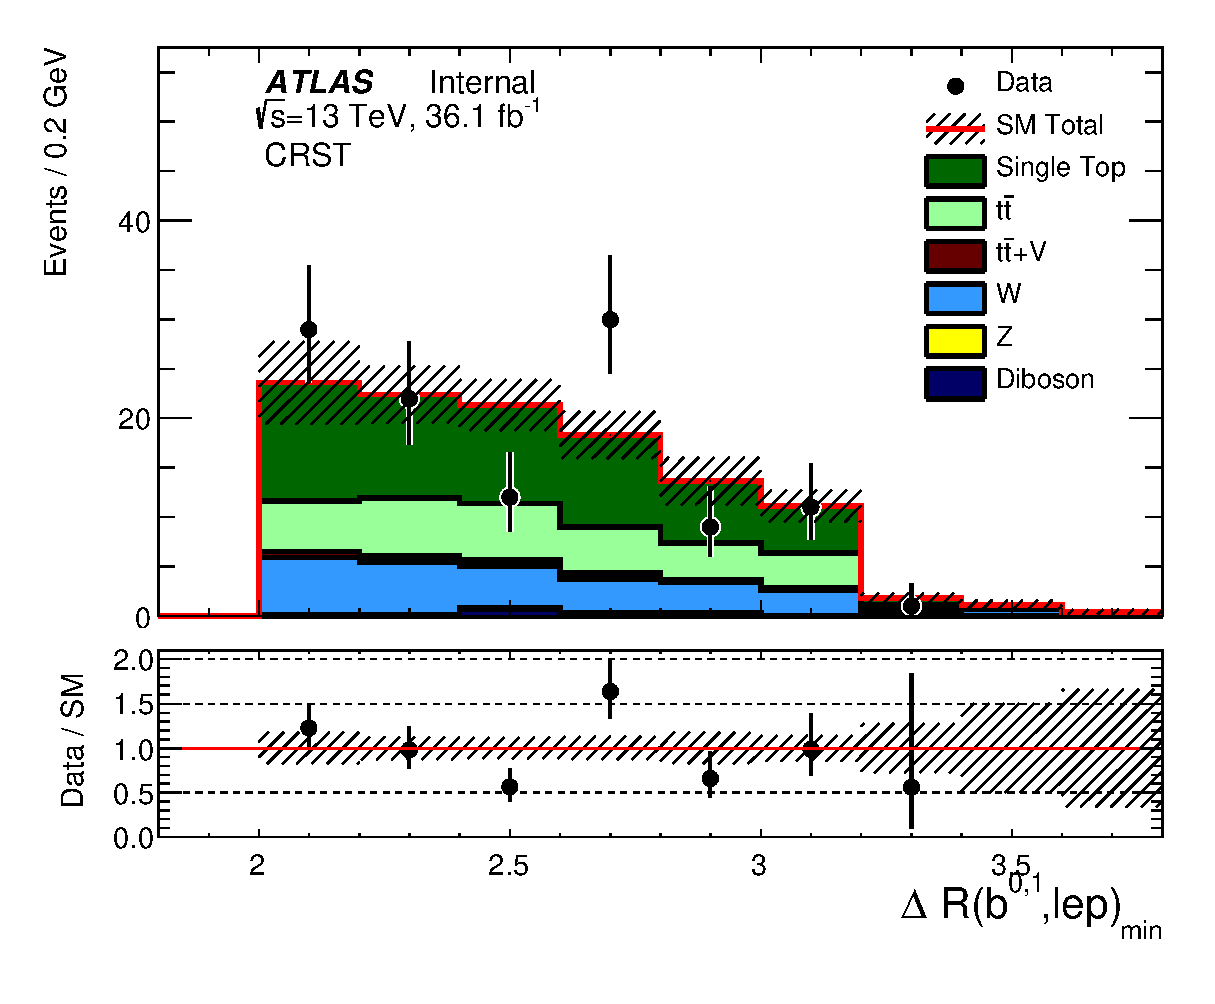
\includegraphics[width=\textwidth]{figures/singleTop/postfit/MinDRBLep_CRST.eps}
                \caption{ }
    \end{subfigure}
      \begin{subfigure}[b]{0.40\textwidth}    
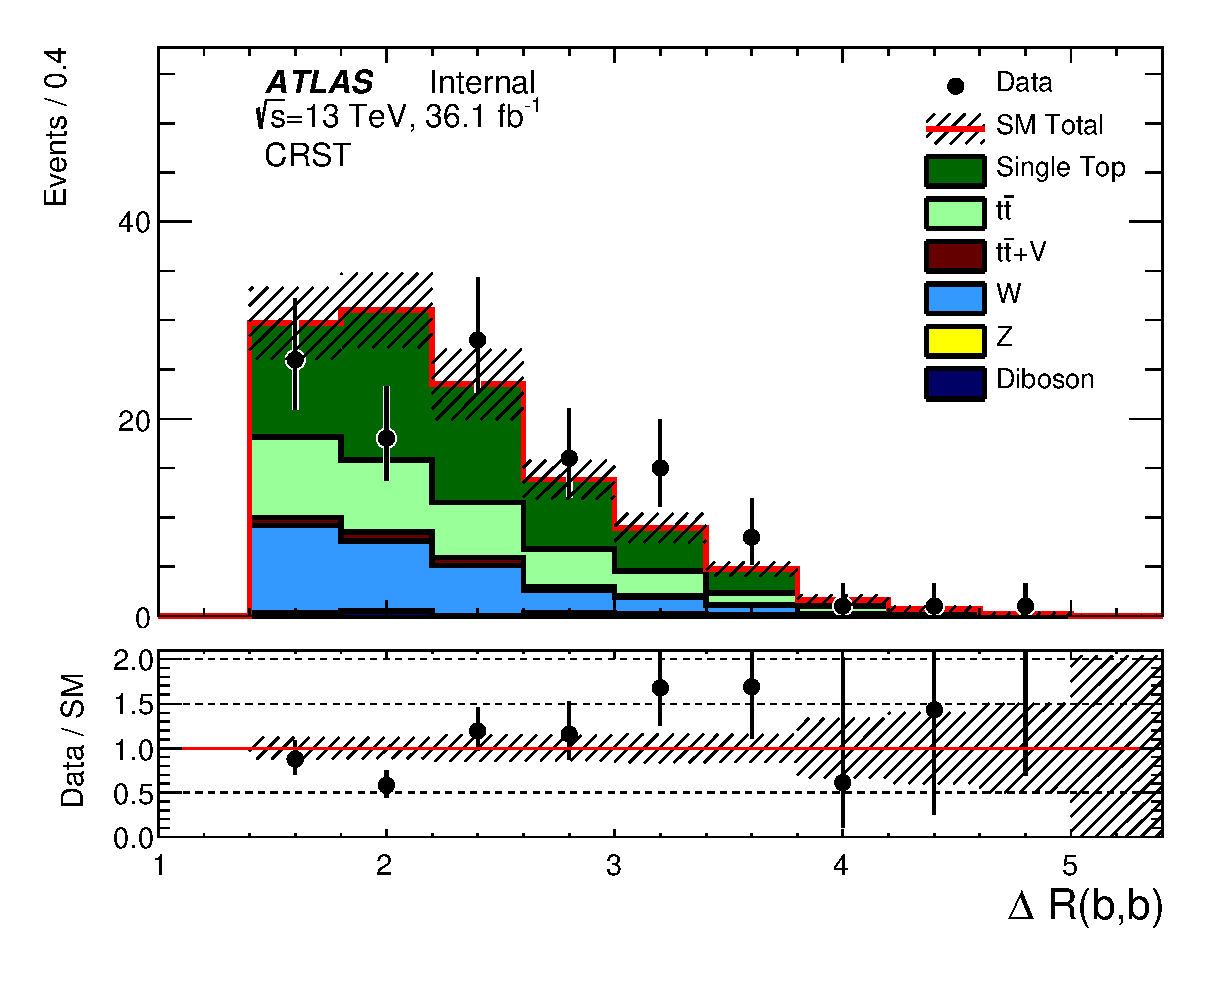
\includegraphics[width=\textwidth]{figures/singleTop/postfit/DRBB_CRST.eps}
                \caption{ }
    \end{subfigure}
%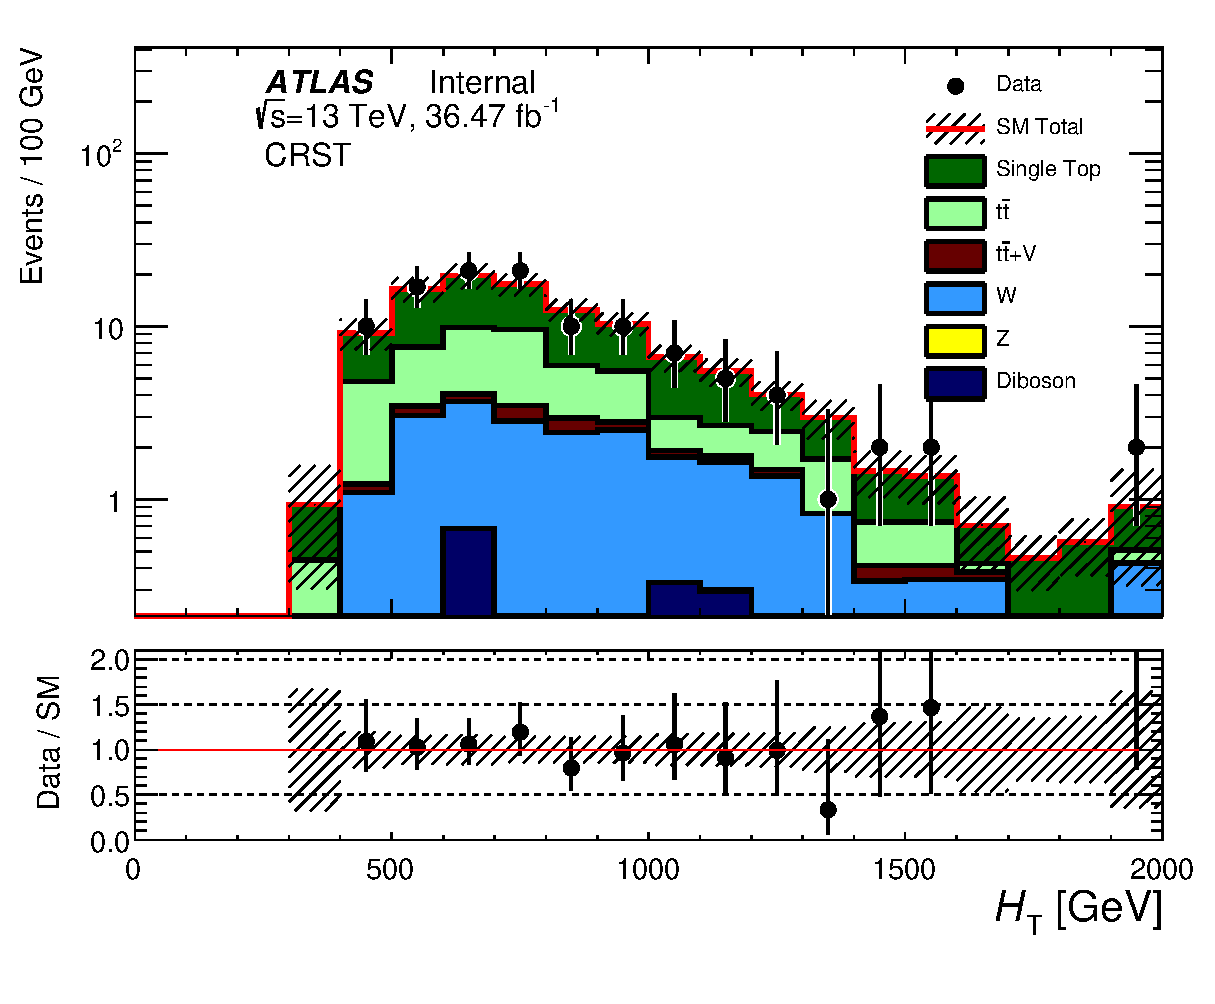
\includegraphics[width=\textwidth]{figures/singleTop/postfit/Ht_CRST_log.eps}
%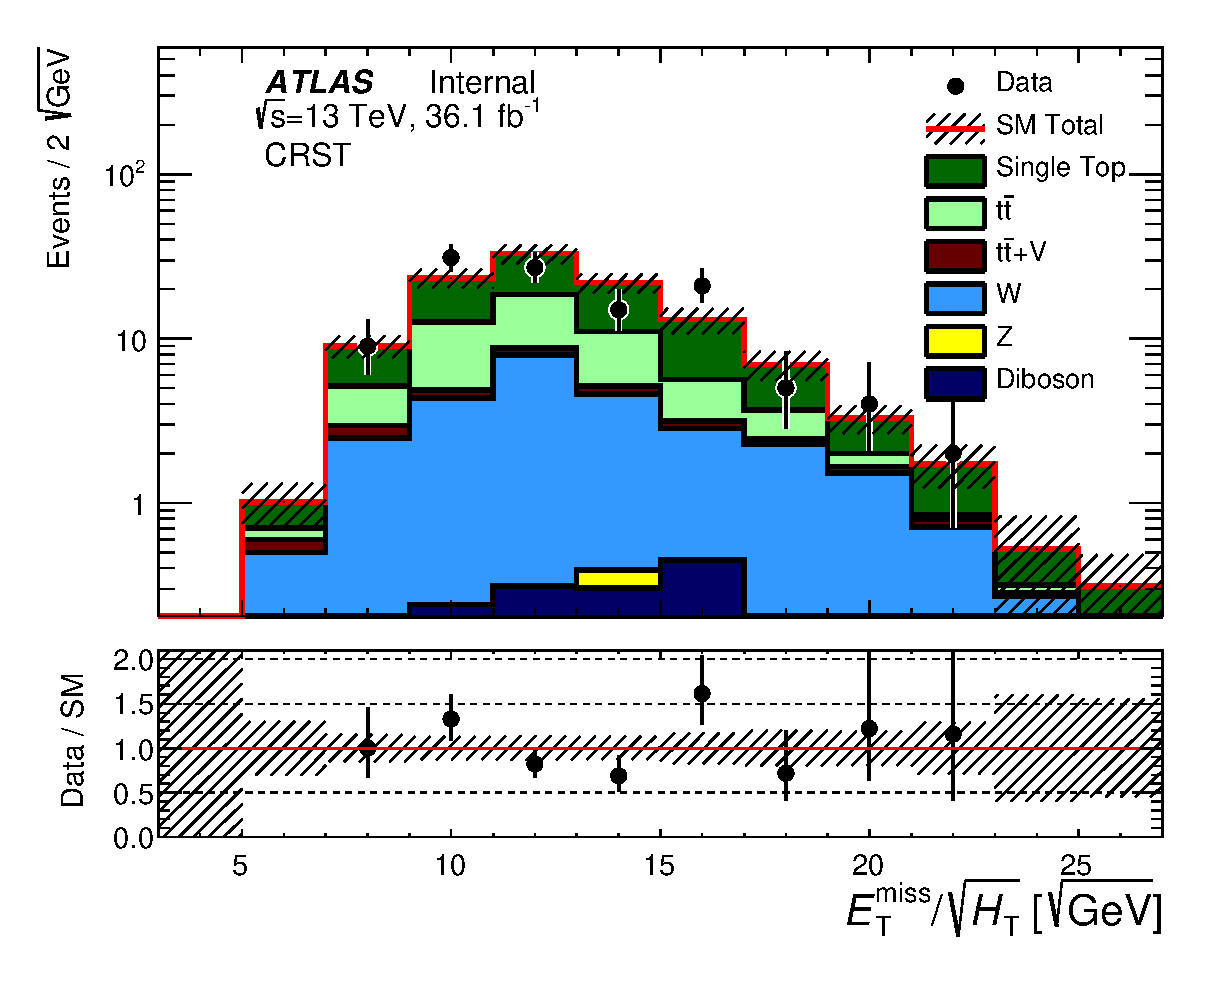
\includegraphics[width=\textwidth]{figures/singleTop/postfit/HtSig_CRST_log.eps}
\end{center}
\caption[~Single-top control region distributions for $\intlumi$ $\ifb$ of data after a simultaneous fit to all control regions]{Single-top control region distributions for $\intlumi$ $\ifb$ of data after a simultaneous fit to all control regions. The kinematic variables include (a) $\met$ (b) number of jets (c) $\mantikttwelvezero$ (d) $\mtbmin$ (e) $\mindrblep$ (f) $\drbjetbjet$. }%The ratio between data and MC is shown in the bottom panel. The hashed area on the expected SM background represents the uncertainty due to experimental systematics and MC statistics.}
\label{fig:CRST}
\end{figure}

\pagebreak

\begin{figure}[h!]
  \begin{center}
      \begin{subfigure}[b]{0.40\textwidth}    
    	 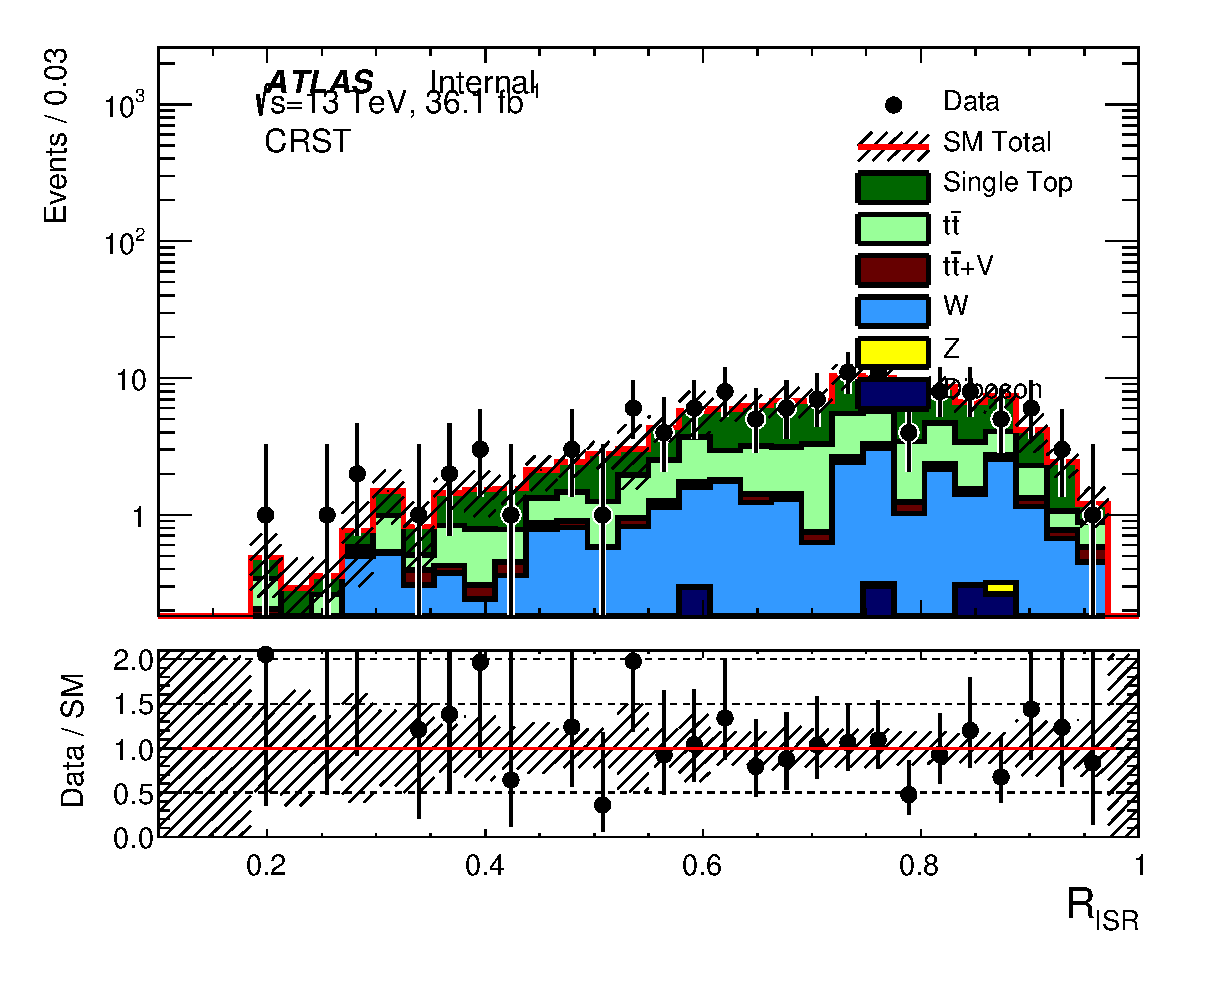
\includegraphics[width=\textwidth]{figures/plotRegion/CA_RISR_CRST_log.eps}
                \caption{ }
    \end{subfigure}
        \begin{subfigure}[b]{0.40\textwidth}    
    	 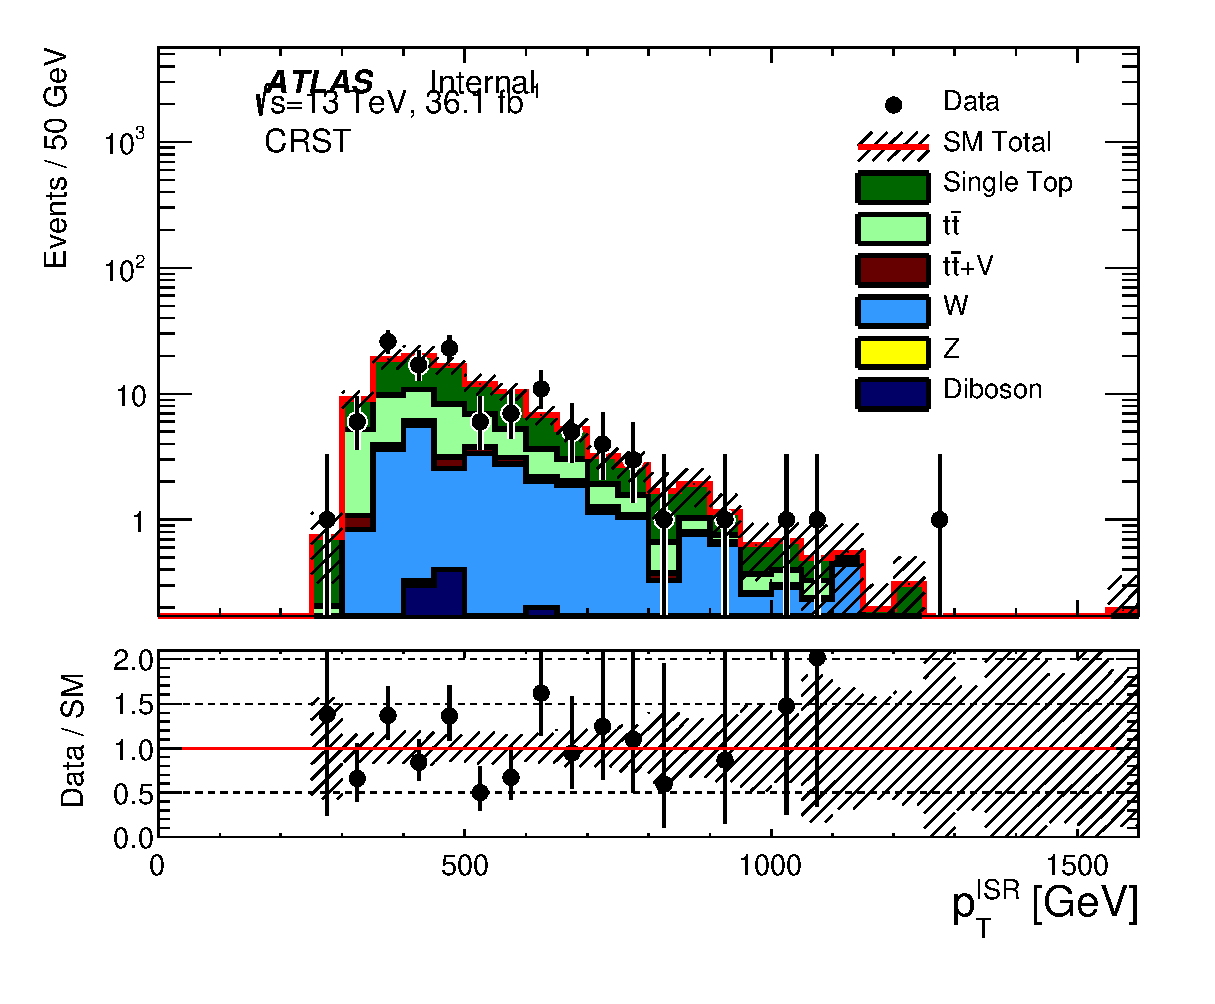
\includegraphics[width=\textwidth]{figures/plotRegion/CA_PTISR_CRST_log.eps}
                \caption{ }
    \end{subfigure}
    \begin{subfigure}[b]{0.40\textwidth}    
    	 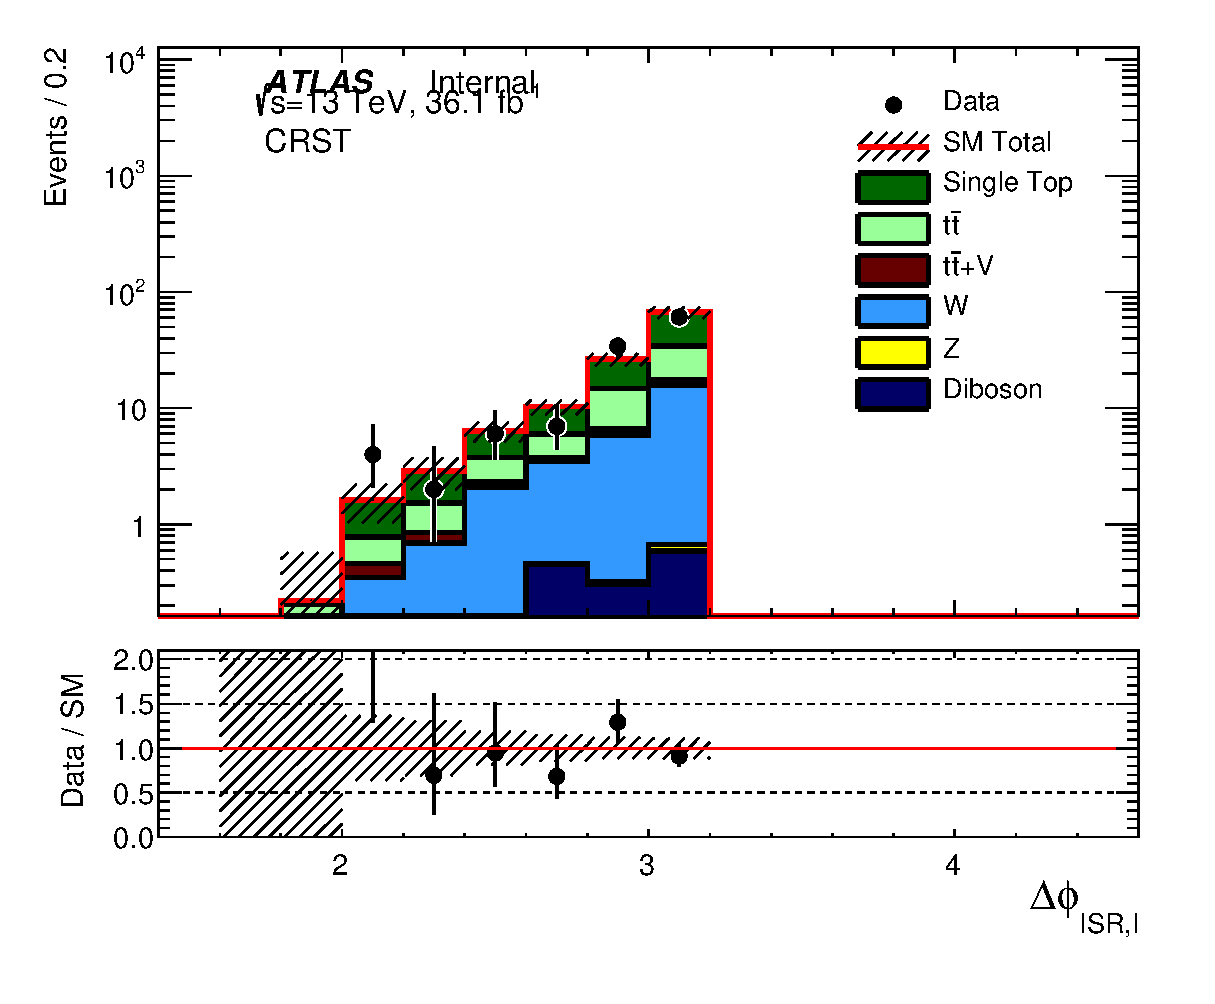
\includegraphics[width=\textwidth]{figures/plotRegion/CA_dphiISRI_CRST_log.eps}
                \caption{ }
    \end{subfigure}
    \begin{subfigure}[b]{0.40\textwidth}    
    	 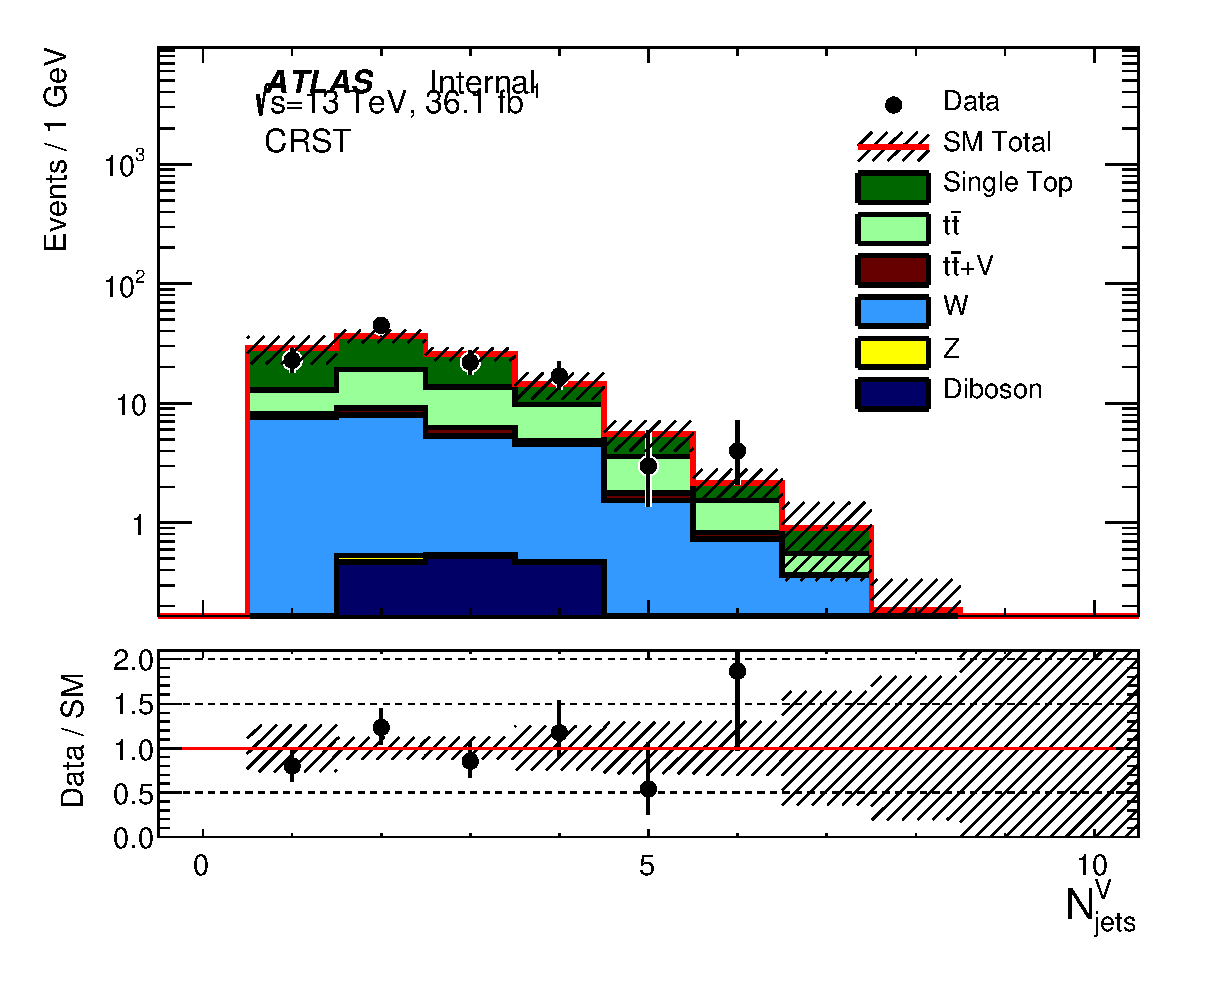
\includegraphics[width=\textwidth]{figures/plotRegion/CA_NjV_CRST_log.eps}
                \caption{ }
    \end{subfigure}
    \begin{subfigure}[b]{0.40\textwidth}    
    	 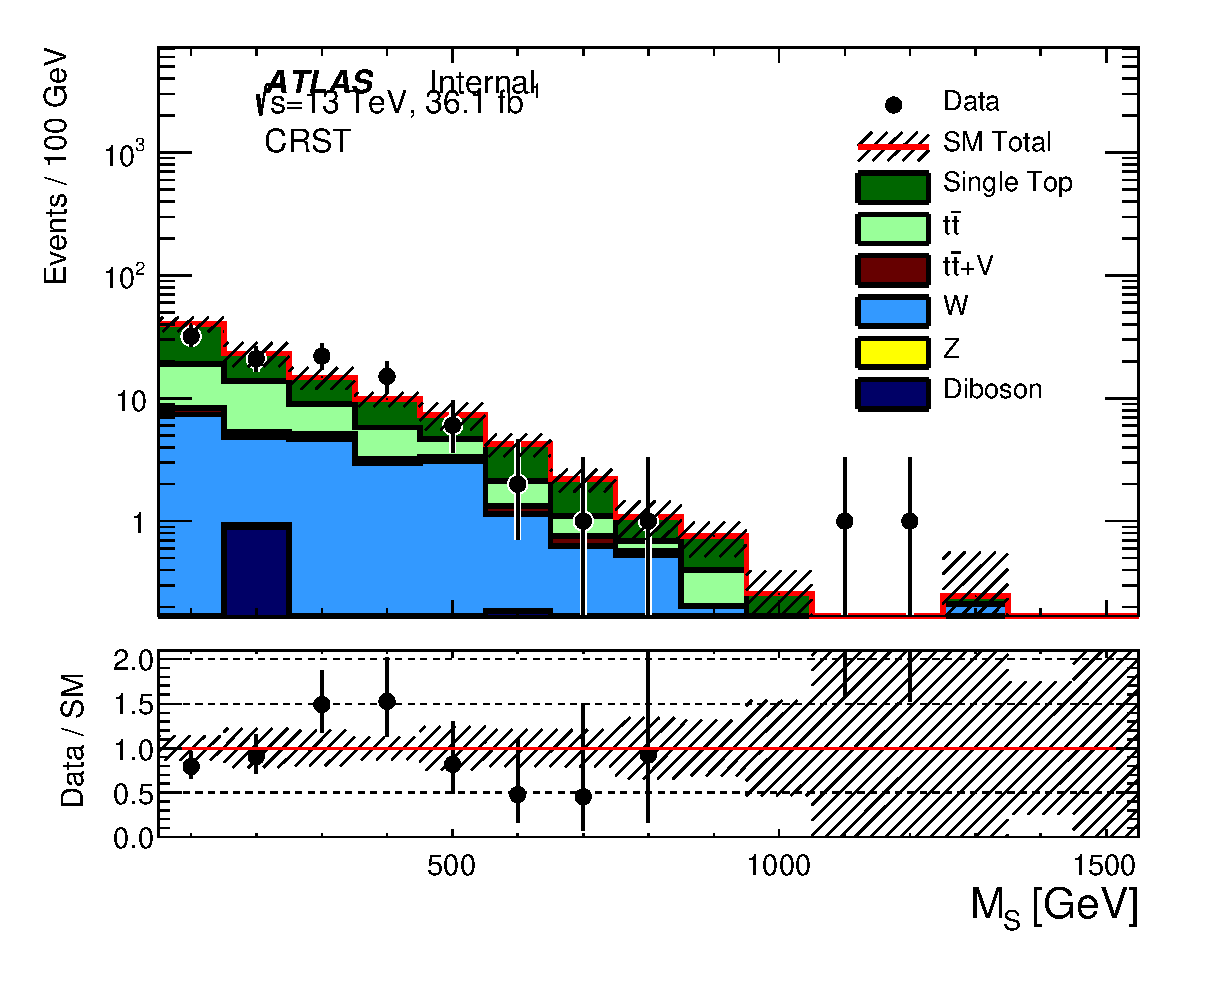
\includegraphics[width=\textwidth]{figures/plotRegion/CA_MS_CRST_log.eps}
                \caption{ }
    \end{subfigure}
    \begin{subfigure}[b]{0.40\textwidth}    
    	 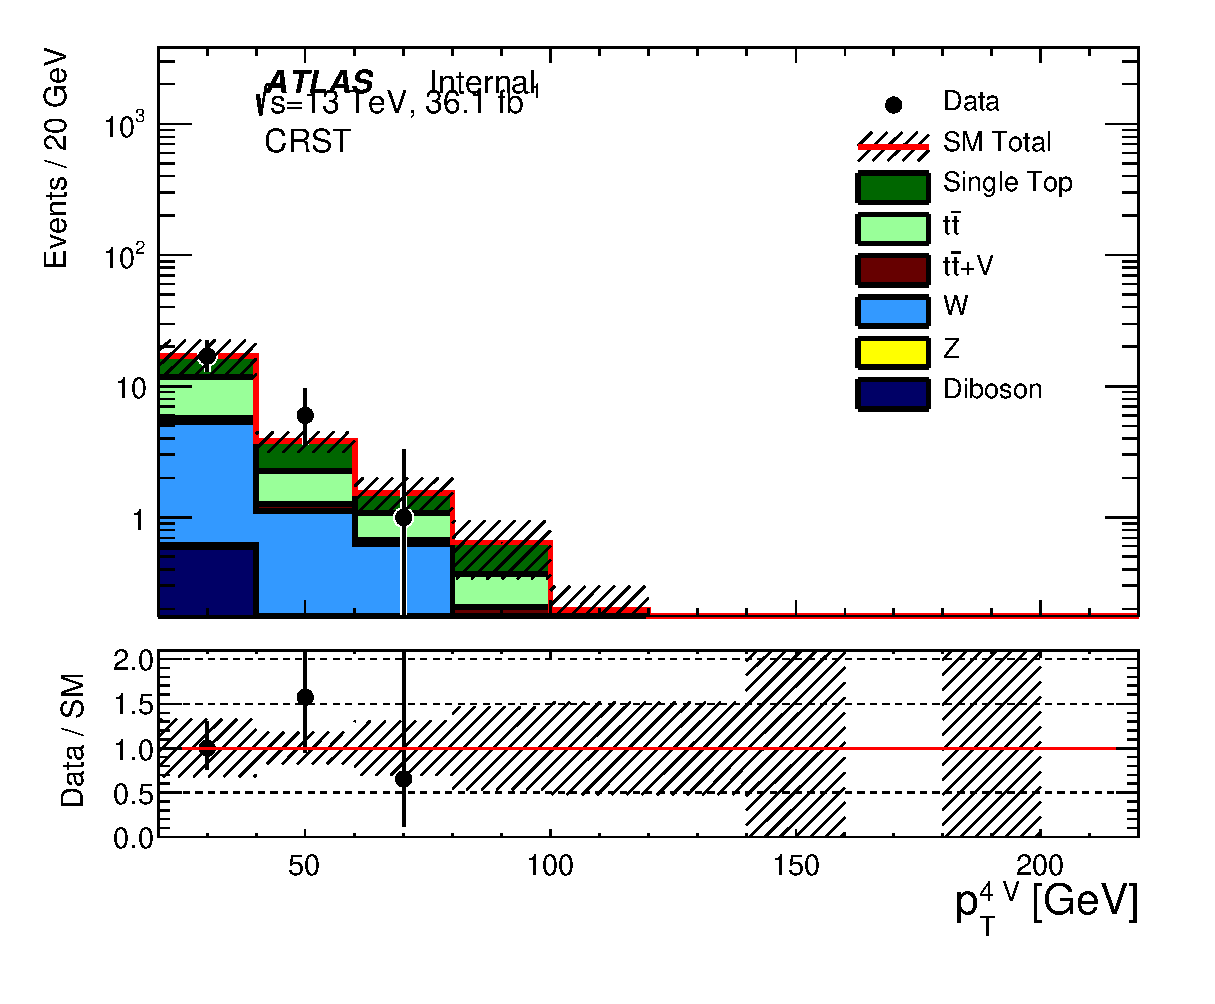
\includegraphics[width=\textwidth]{figures/plotRegion/CA_pTjV4_CRST_log.eps}
               \caption{ }
    \end{subfigure}
     \caption[~Single-top control region distributions for \intlumi\ \ifb\ of data after a simultaneous fit to all control regions.]{ Single-top control region distributions for \intlumi\ \ifb\ of data after a simultaneous fit to all control regions. The kinematic variables include (a) $\RISR$ (b) $\PTISR$ (c) $\dphiISRI$ (d) $\NjV$ (e) $\MS$ (f) $\pTjV$.  }%The ratio between data and MC is shown in the bottom panel. The hashed area on the expected SM background represents the uncertainty due to experimental systematics and MC statistics.}
     
  \label{fig:CRST1}
    \end{center}
\end{figure}

\pagebreak



\begin{table}[h!]
\caption[Single top control region MC Yield and background-only fit results for $\intlumi$ $\ifb$ of data]{Single top control region MC Yield and background-only fit results for $\intlumi$ $\ifb$ of data. MC exp. events are expected background rates directly from MC predictions.  Fitted background event rates are the expected background rates after normalizing the MC to data by simultaneously fitting all control regions using a background only fit.  The fitted $W$+jets normalization scale factor is equal to (Fitted single top events)/(MC exp. single top events). The quoted uncertainties include statistical and systematic uncertainties. }
\label{table.bkgonly.CRST}
\begin{center}
\setlength{\tabcolsep}{0.0pc}
{\small
%%
\begin{tabular*}{\textwidth}{@{\extracolsep{\fill}}lr}
\noalign{\smallskip}\hline\noalign{\smallskip}
{\bf CRother yields}             & CRST              \\[-0.05cm]
\noalign{\smallskip}\hline\noalign{\smallskip}
%%
Observed events                & $114$                    \\
\noalign{\smallskip}\hline\noalign{\smallskip}
%%
Fitted bkg events                & $113.93 \pm 10.65$              \\
\noalign{\smallskip}\hline\noalign{\smallskip}
%%
        Fitted TTbar events              & $29.80 \pm 10.52$              \\
%%
        Fitted Wjets events           & $26.36 \pm 5.82$              \\
%%
        Fitted Zjets events              & $0.10 \pm 0.07$              \\
%%
        Fitted TtbarV events             & $3.14 \pm 0.73$              \\
%%
        Fitted SingleTop events            & $52.95 \pm 17.45$              \\
%%
        Fitted Diboson events                & $1.59 \pm 0.79$              \\
%%
        Fitted Multijets events                & $0.00 \pm 0.00$              \\
%%     
 \noalign{\smallskip}\hline\noalign{\smallskip}
%%
MC exp. SM events                    & $102.60 \pm 12.42$              \\
\noalign{\smallskip}\hline\noalign{\smallskip}
%%
        MC exp. TTbar events             & $32.24 \pm 11.17$              \\
%%
        MC exp. Wjets events             & $20.83 \pm 3.02$              \\
%%
        MC exp. Zjets events                & $0.09 \pm 0.06$              \\
%%
        MC exp. TtbarV events              & $2.44 \pm 0.42$              \\
%%
        MC exp. SingleTop events            & $45.42 \pm 1.32$              \\
%%
        MC exp. Diboson events                & $1.58 \pm 0.79$              \\
%%
        MC exp. Multijets events             & $0.00 \pm 0.00$              \\
%%     \\
\noalign{\smallskip}\hline\noalign{\smallskip}
Fitted single top normalization scale factor & $0.707 \pm 0.050$ \\
\noalign{\smallskip}\hline\noalign{\smallskip}
\end{tabular*}
%%%
}
\end{center}
\end{table}
%


\subsection{Standard Model \ttbar+Z}
\label{sec:Bkg:ttV}

\indent ttbar produced in conjunction with a Z boson consist of about one percent of the background in the SR.  Although the background is essentially negligible we do estimate the amount of $\ttbar+\Zboson$ using a $\ttbar+\gamma$ CR. \\

\indent Using the charged leptonic $Z$ boson decays to design a CR to estimate the $\ttbar+Z$ background would produce a CR with small systematic uncertainty. However, such CR tend to have low statistics because of the small branching fraction to electrons/muons compared to the branching fraction of neutrinos.  A dilepton CR also contain a large contribution from SM ttbar and $Z$ + jets. \\

\indent We take another data driven approach by building a one-lepton CR for $\ttbar+\gamma$.  $\ttbar+\gamma$ mimics $\ttbar+Z$ as the photon is in many ways like a lighter $Z$ boson.  The CR is designed to minimize theoretical uncertainties due to the extrapolation from the $\gamma$ in CR to the $\Zboson$ in SR. \\

\indent We require exactly one {\tt Signal} photon and one {\tt Signal} lepton.  The lepton is not treated as a jet for the purpose of jet multiplicity and jet $\pt$ requirements unlike in the other one lepton CRs.  We also trigger on leptons instead of $\met$ in this region. The lepton triggers used are defined in table \ref{tb:lepTriggers}.  \\

\begin{table}[htpb]
  \caption{Single Lepton triggers}
  \begin{center}
    \begin{tabular}{c|c} \hline\hline
      Channel & Trigger \\  \hline
              & {\bf Data 2015} \\ \hline
      Electron & \verb+HLT_e24_lhmedium_L1EM20VH+  \\
      	            & \verb+HLT_e60_lhmedium+ \\
	            & \verb+HLT_e120_lhloose+         \\  
      Muon & \verb+HLT_mu20_iloose_L1MU15+ \\
      	       & \verb+HLT_mu50+ \\
      \hline
              & {\bf Data 2016} \\ \hline
      Electron & \verb+HLT_e26_lhtight_nod0_ivarloose+ \\
                     &\verb+HLT_e60_lhmedium_nod0+ \\
                     &\verb+HLT_e140_lhloose_nod0+         \\ 
      Muon & \verb+HLT_mu26_ivarmedium+ \\ 
                & \verb+HLT_mu50+ \\
      \hline \hline
    \end{tabular}
  \end{center}
  \label{tb:lepTriggers}
\end{table}


\indent We require a hight $\pt$ photon with $\pt$ greater than $150\gev$.  The high $\pt$ gamma ensures that we are in a region of phase space where the $\gamma$ $\pt$ shape will mimic the heavier $\Zboson$ $\pt$.  The true $\gamma$ $\pt$ and the $\Zboson$ $\pt$ distributions is shown in figure \ref{fig:ttZ_vs_ttGamma_pt} after selecting for a boson $\pt$ with greater then $150 \gev$.  We add a systematic uncertainty to account for the difference between the $\gamma$ and $\Zboson$ $\pt$ spectrum. \\

\begin{figure}[htpb]
\centering
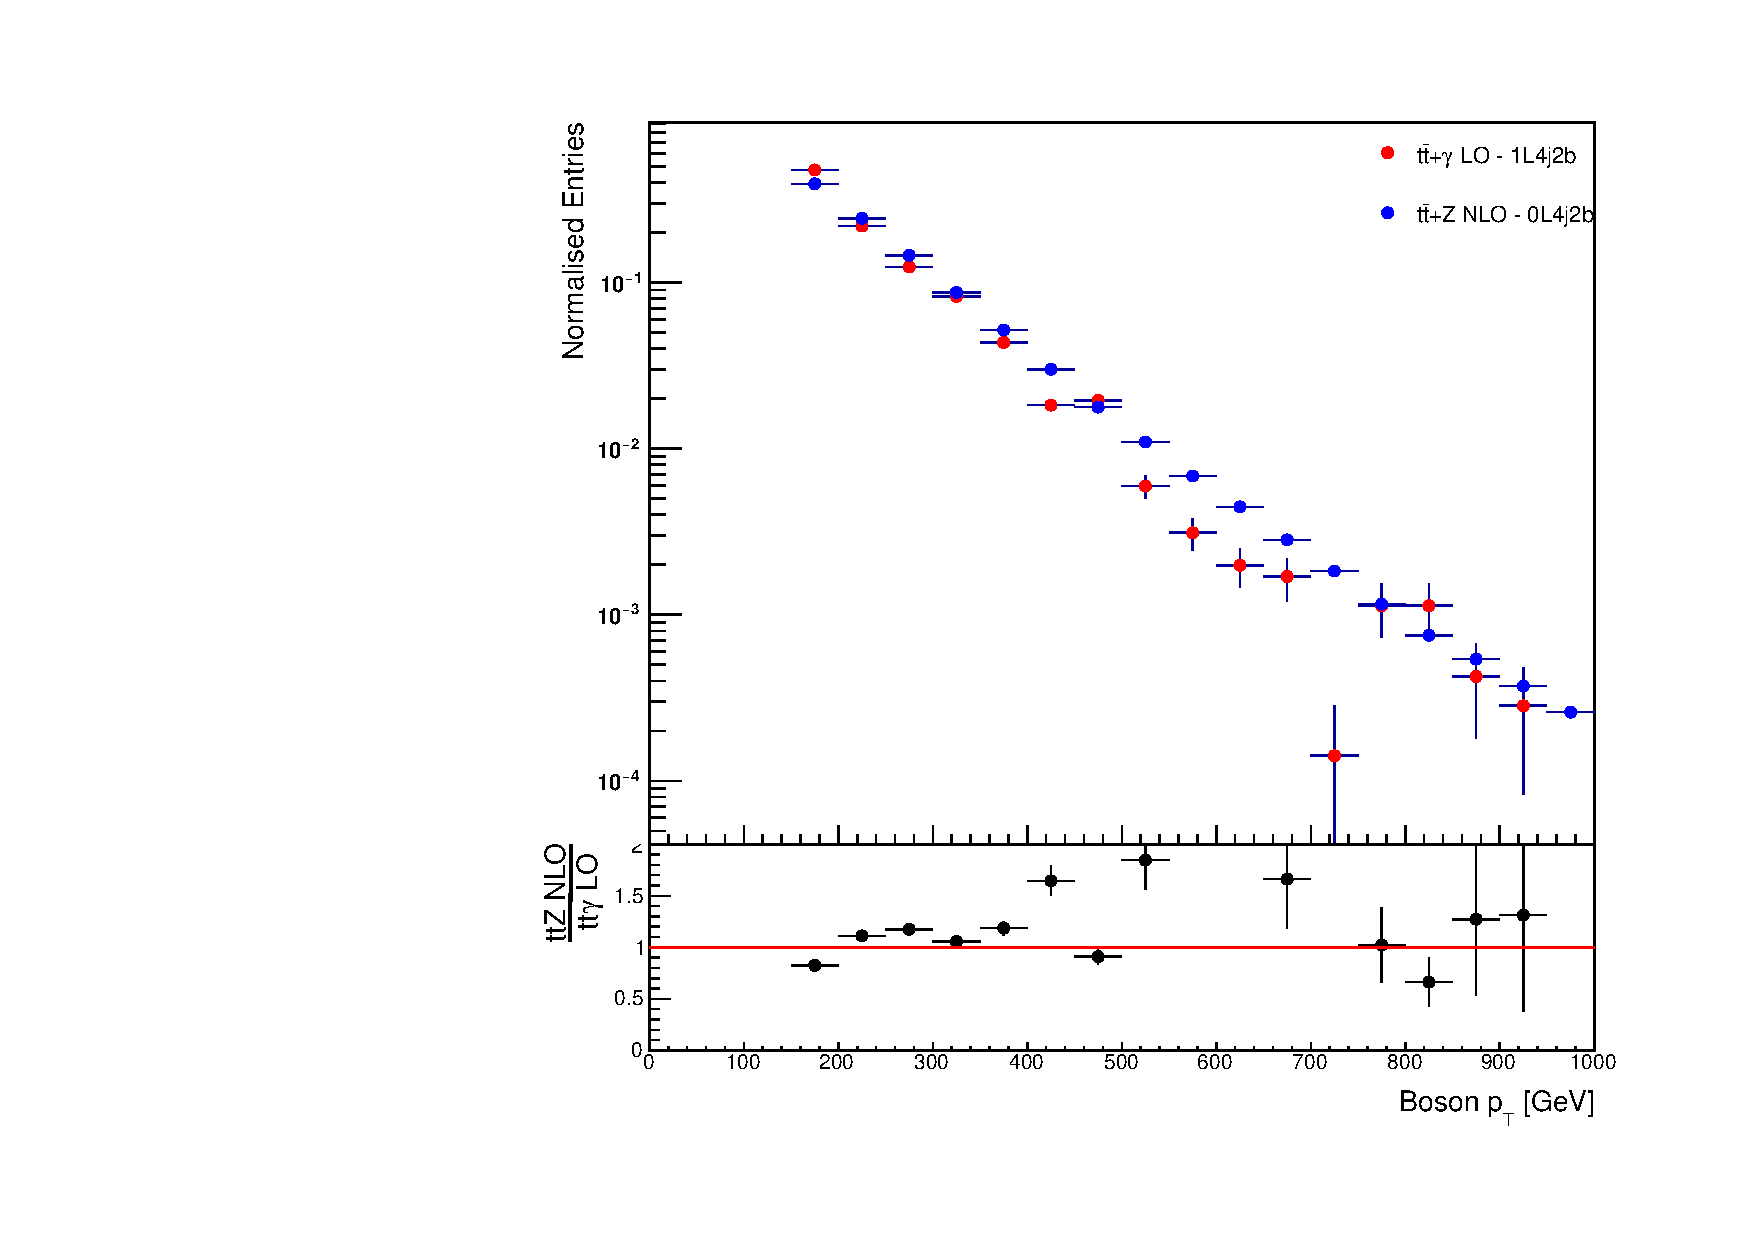
\includegraphics[scale=0.4, angle=270]{figures/ttGamma/TruthStudies/Pt150.pdf}
\caption{$\gamma$ and $\Zboson$ $\pT$ distributions with no detector resolution effects.  A selection of $\pt > 150 \gev$ has been applied.}
\label{fig:ttZ_vs_ttGamma_pt}
\end{figure}

\indent The $\ttbar+\gamma$ control region is defined in table~\ref{tb:ttG_1lepSel}.  The expected background and data yields in the $\ttbar+\gamma$ CR is given in table \ref{tb:ttVCR_2bj}. \\


\begin{table}[htpb]
  \begin{center}
    \begin{tabular}{c|c}
      \hline \hline
      Selection                 & Requirement     \\
      \hline \hline
      Event selection & Event cleaning \\
      \hline
       Trigger  & 1L Triggers  \\  \hline
      Leptons & $= 1$ \\
      Lepton \pt & 28 $\GeV$ \\
      \hline
      Photons & exactly 1\\
      \hline
      jet multiplicity & $ \ge 4 $ \\
      \hline
      Jet \pT\ & (80,80,40,40) GeV \\
      \hline
      b-jet multiplicity & $\ge 2$ \\
      \hline
      $\gamma$ \pT\ & $> 150$ GeV \\
      \hline\hline
    \end{tabular}
  \end{center}
    \caption{Selection for the $\ttbar+\gamma$ one lepton CR. The one lepton triggers as described in Table~\ref{tb:lepTriggers}}
      \label{tb:ttG_1lepSel}
\end{table}


\begin{table}[htpb]
  \caption{Background composition of $t\bar{t}\gamma$ CR.}
  \begin{center}
\begin{tabular}{c|c}
\hline\hline
\multicolumn{2}{c}{\bf CRTTGamma (87\% purity)} \\ \hline 
ttGamma & 112.20 $\pm$ 1.49 \\
VGamma & 6.41 $\pm$ 0.70 \\
Z & 0.73 $\pm$ 0.21 \\
dibosons & 0.00 $\pm$ 0.00 \\
ttbar & 4.57 $\pm$ 1.23 \\
singleTop & 2.01 $\pm$ 0.81 \\
ttV & 2.42 $\pm$ 0.28 \\
W & 0.04 $\pm$ 0.02 \\
\hline
Total MC & 128.38 $\pm$ 2.23 \\
Data & 160.00 $\pm$ 12.65 \\
 \hline
SF & 1.28 $\pm$ 0.12 \\
\hline\hline
\end{tabular}

    
  \end{center}
  \label{tb:ttVCR_2bj}
\end{table}

\indent Kinematic distributions in the $\ttbar+\gamma$ control region are shown in figure ~\ref{fig:ttgamma}  The MC background has been normalized to data by performing a simultaneous fit to all CRs.  The hashed bands on the total SM background correspond to the total experimental systematical uncertainty plus the MC statistical uncertainty.   \\

\begin{figure}[htbp]
\begin{center}
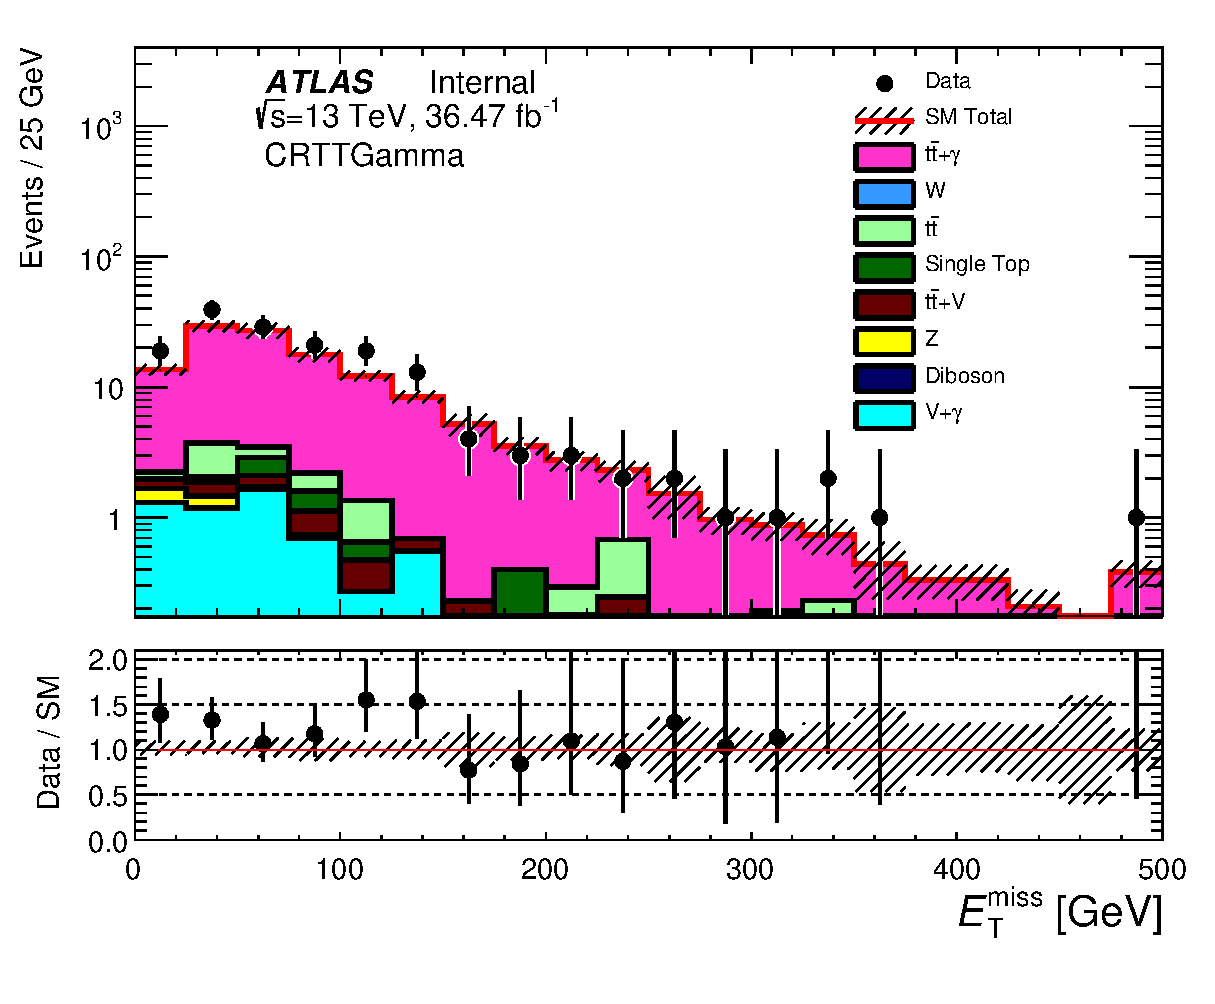
\includegraphics[width=0.49\textwidth]{figures/ttGamma/Met_CRTTGamma_withRatio_log.eps}
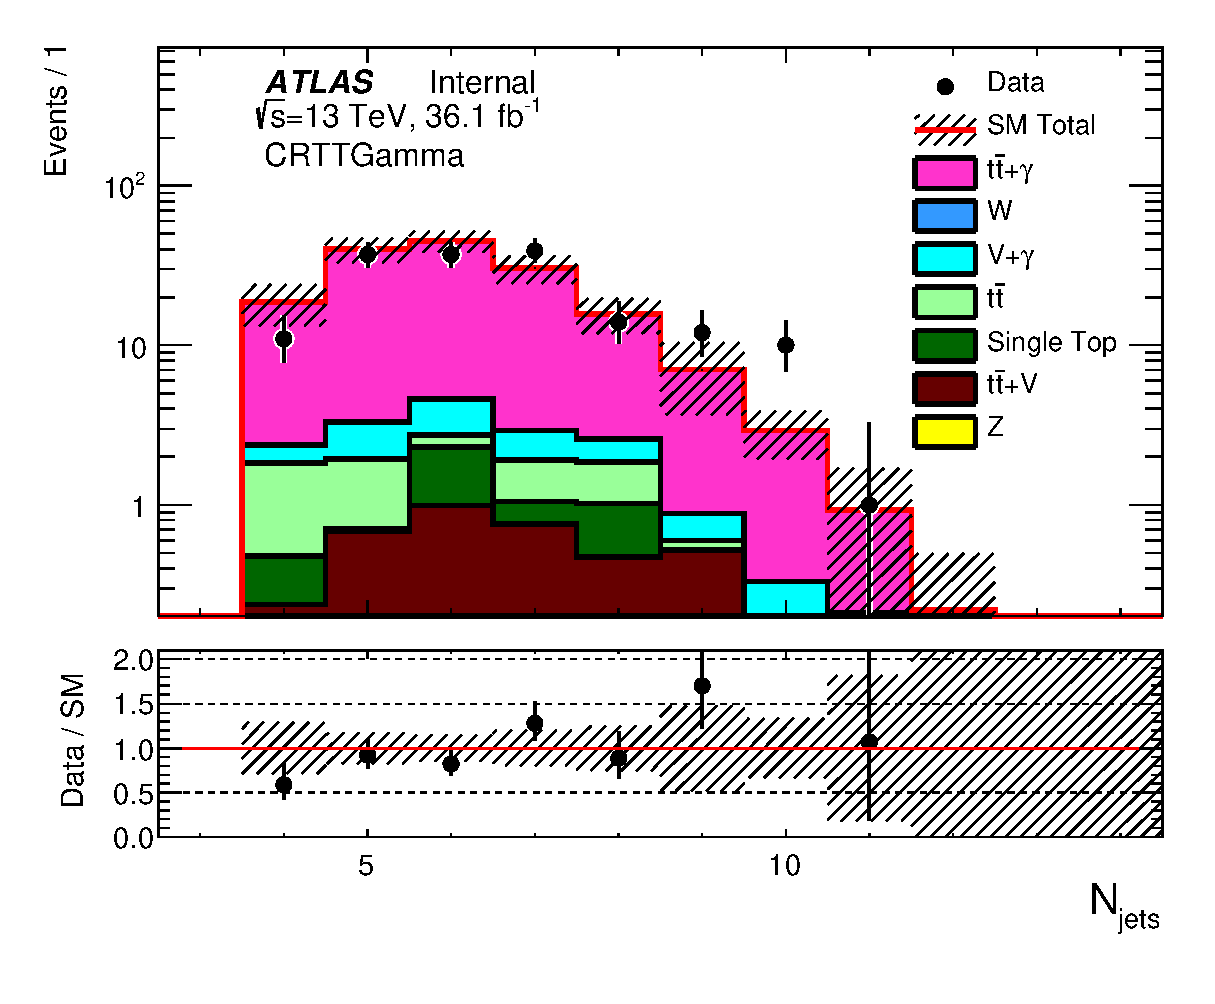
\includegraphics[width=0.49\textwidth]{figures/ttGamma/postfit/NJets_CRTTGamma_log.eps}
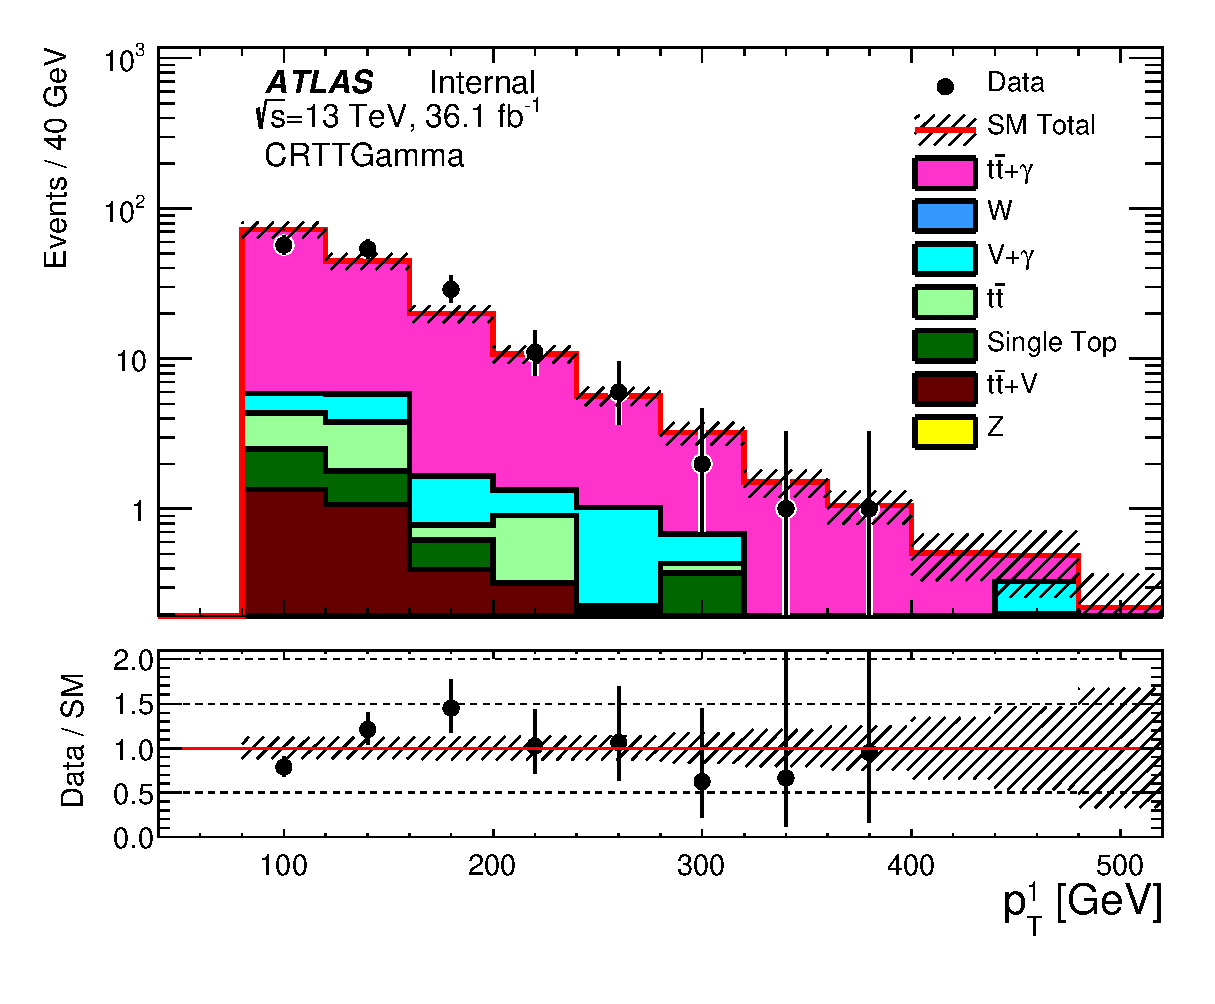
\includegraphics[width=0.49\textwidth]{figures/ttGamma/postfit/JetPt_1__CRTTGamma_log.eps}
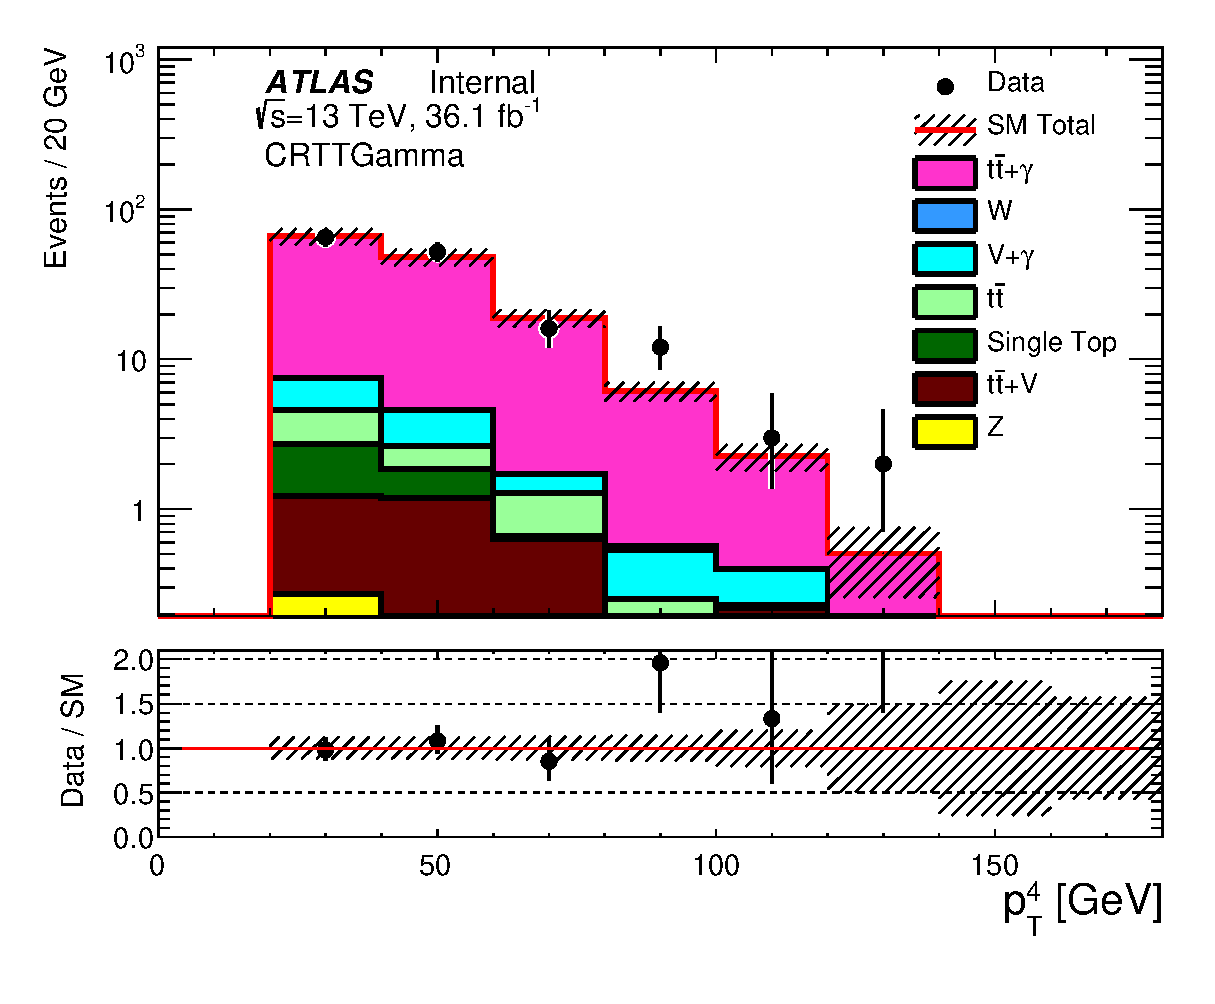
\includegraphics[width=0.49\textwidth]{figures/ttGamma/postfit/JetPt_4__CRTTGamma_log.eps}
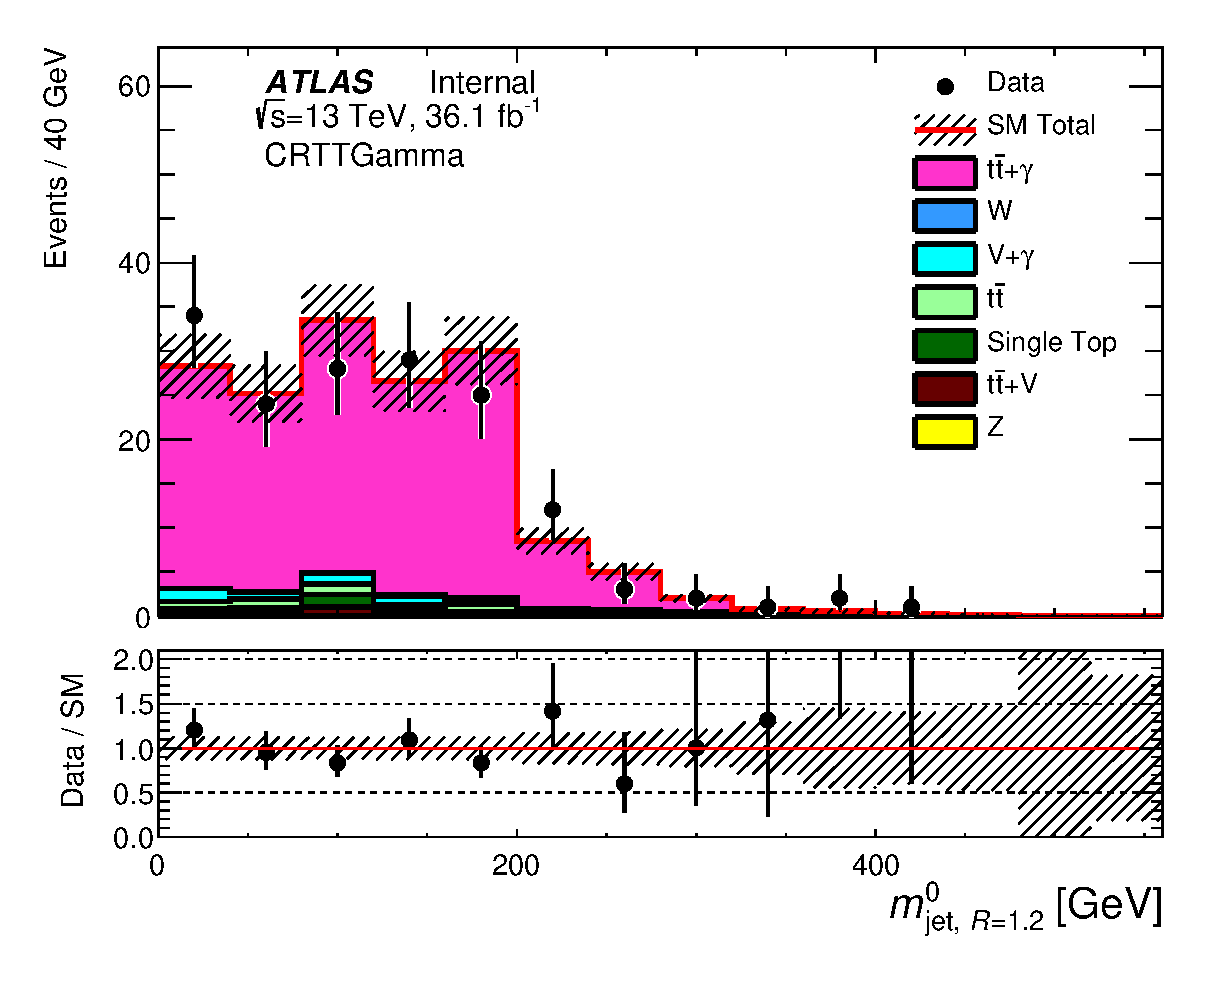
\includegraphics[width=0.49\textwidth]{figures/ttGamma/postfit/AntiKt12M_0__CRTTGamma.eps}
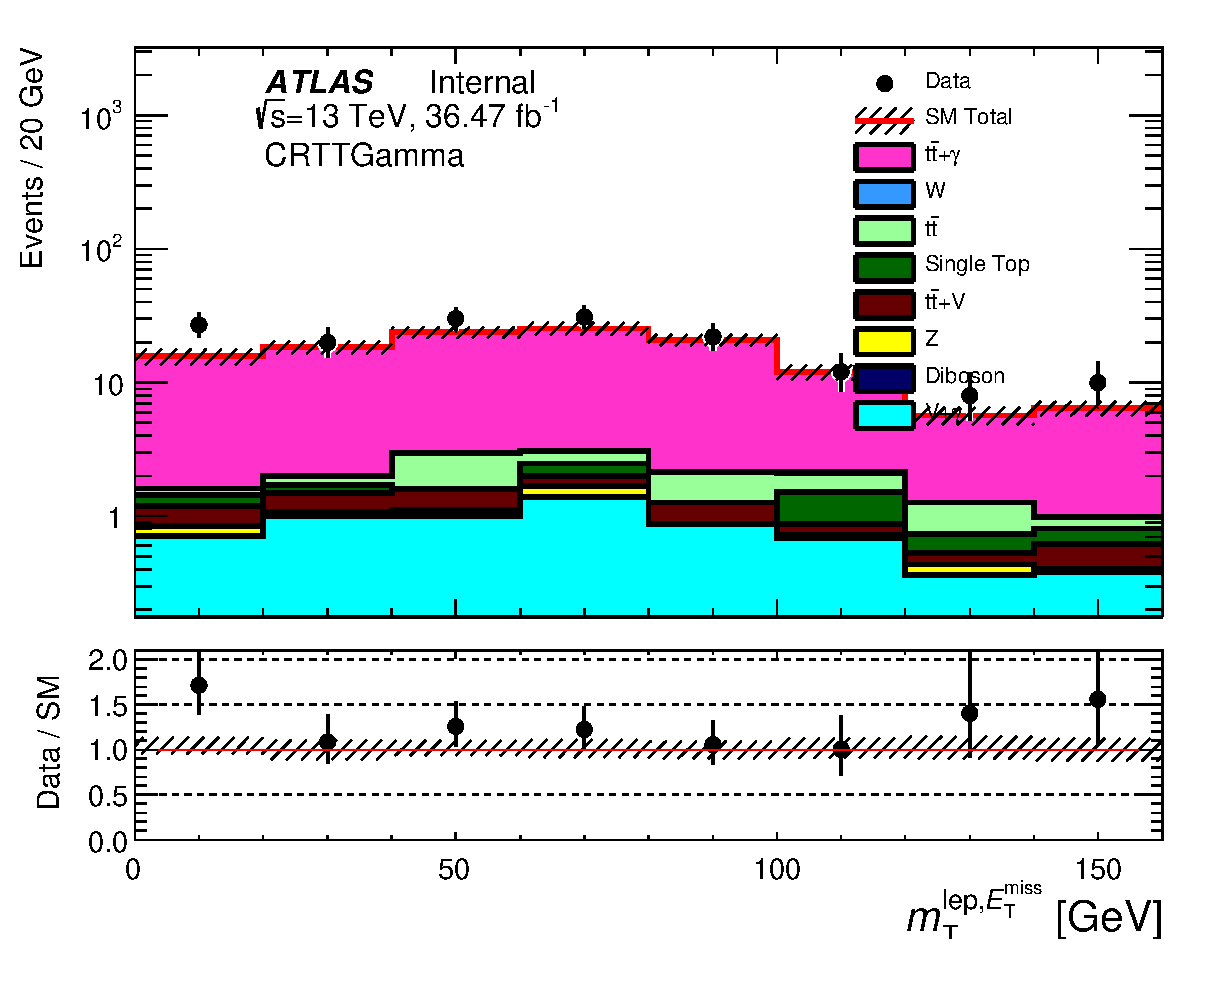
\includegraphics[width=0.49\textwidth]{figures/ttGamma/MtMetLep_CRTTGamma_withRatio_log.eps}
\caption{\label{fig:ttgamma} Distributions of select kinematic variables in the $\ttbar+\gamma$ CR. The hashed area in both the top and lower panel represents the uncertainty due to MC statistics.}
\label{fig:ttgamma}
\end{center}
\end{figure}







\subsection{Standard Model Z+Jets}
\label{sec:Bkg:zjet}

Z+jets consist of 3 percent of all backgrounds in the SR.  The percentage of Z+jets is higher in high $\RISR$ bins.  The percentage Z+jets rises to 7 percent in $\RISR$ between 0.6 and 0.8.  We use just the MC prediction for Z+jets because the rate of Z+jet is so low.  We assign an 100 percent theory uncertainty to the Z+jets rate in the SR.  \\
The ttbar validation region described in section \ref{sec:Bkg:ttbar:VR} has a larger fraction of Z+jets event then those in the SR.  The ttbar VR is kinematically similar to those of the SR with some loser cuts on jet multiplicity and ISR, \MET correlations.  The good agreement between data and MC in the ttbar VR is evidence that the Z+jets MC cannot be wrong by more than 100 percent.  \\
\subsection{Standard Model Diboson}
\label{sec:Bkg:diboson}

\indent Standard Model dibosons consist of approximately 1\% of the background in the signal region.  The background is negligible and we only use MC predictions for background estimation. We apply a 50\% theory uncertainty on the diboson background. \\
\subsection{Standard Model QCD Multijet}
\label{sec:Bkg:QCD}

\indent  QCD multijet events form a significant contribution to background rates in signal region bins with $\RISR < 0.4$.  The QCD multijet process creates little intrinsic $\met$ from actual neutrinos. Instead, misreconstructed jets are the primary reason why some QCD multijet events are able to pass the $\met > 250 \gev$ requirement and the signal region selections.  Misreconstructed jets can cause an imbalance in the total event $E_t$ and lead to events with a large reconstructed $\met$ even if the event has little intrinsic $\met$.  We estimated the QCD background using the data driven {\tt Jet Smearing} method.   \\

\subsubsection{The {\tt Jet Smearing} Method of Estimating QCD Background}

\indent The {\tt Jet Smearing} method first selects seed events from data with well reconstructed jets and little $\met$.  We then repeatedly smear the seed events' jets with a predetermined jet energy response.  The resulting {\tt pesudo-data} events can have potentially large $\met$ due to the smeared jets.  A schematic demonstrating the {\tt jet smearing} method is shown in Figure \ref{fig:jetsmearing}.\\

\begin{figure}[h!]
\begin{center}
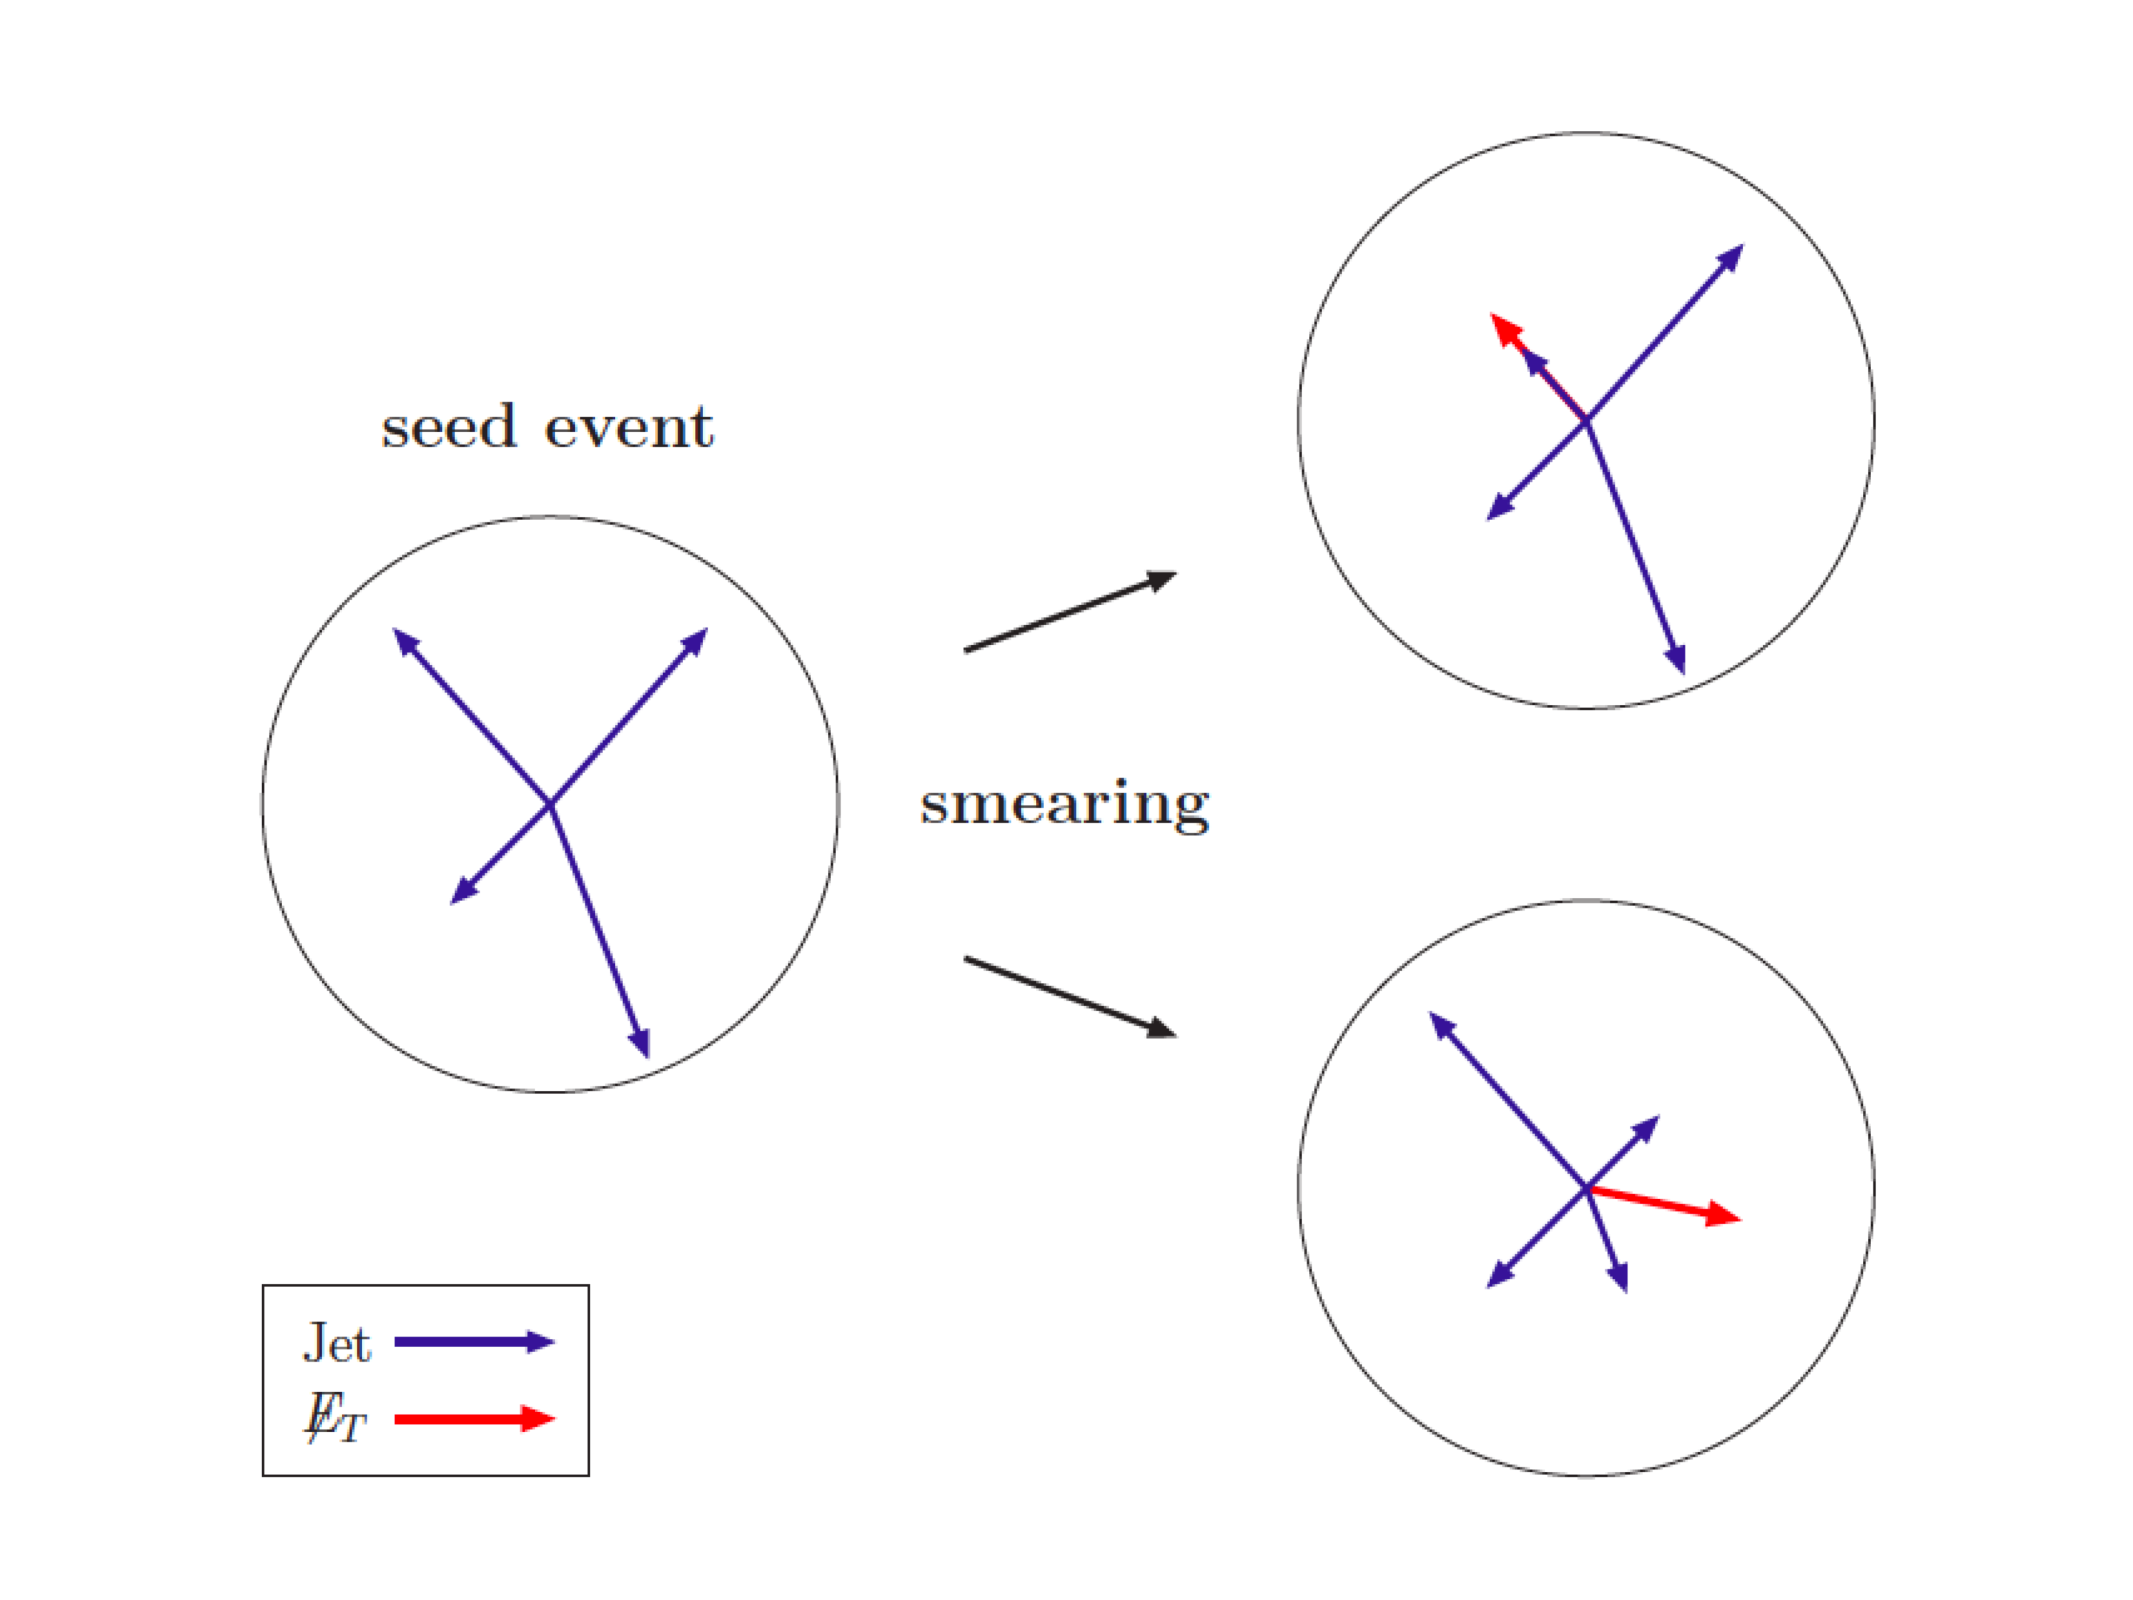
\includegraphics[width=0.45\textwidth]{figures/QCDJetSmearing/jet_smearing.pdf}
\end{center}
\caption[Schematic diagram demonstrating the {\tt Jet Smearing} method of estimating QCD background]{Schematic diagram demonstrating the {\tt Jet Smearing} method of estimating rate of QCD background.  Seed events with good jet energy measurements are repeatedly smeared with predetermined jet energy resolutions.  The new $\met$ is calculated as the difference between the seed event's and smeared event's jet momentum plus the original seed event's $\met$.\cite{JetSmearing} }
\label{fig:jetsmearing}
\end{figure}

\indent The {\tt Jet Smearing} methods have a number of inherent assumptions about the generation of $\met$ in QCD multijet background.  These assumptions include: \\

\begin{itemize}
\item The jet response captures all sources of jet $\pt$ measurement fluctuations
\item The $\met$ in multijet events result predominately from mis-measured jets
\item Jet response is independent on the presence of other jets and jet smearing can be applied on a jet-by-jet basis
\end{itemize}

\indent These assumptions seem to be well satisfied in the high $\met$, high jet multiplicity environment of the signal region.  Other sources of $\met$ not taken into account by the jet smearing method such as $\met$ from pileup jets, mis-reconstructed soft term of the $\met$ and object overlap removal are assumed to be negligible in the signal region. \\

\indent We then define a QCD control region that is kinematic similar to the signal region but dominated by QCD background.  We normalize the predicted QCD rate to the amount of data in the control region.  The normalization factor is then applied to predicted QCD rates in the signal region.  We also validate the QCD predictions using a QCD validation region.  The QCD control and validation regions are covered in greater details in section \ref{sec:QCD:CR}. \\

\subsubsection{{\tt Jet Smearing} Seed Event Selection and Jet Response Function}

\indent We select for events with multiple well reconstructed jets and no leptons as seed events.  Because QCD multijet events have low intrinsic $\met$, seed events must have low $\met$ relative to the total reconstructed $E_T$ in the event. \\ 

\indent Some $\met$ is expected even in well reconstructed multijet events because both the electromagnetic and hadronic calorimeters at ATLAS are sampling calorimeters.  The energy deposited in the absorber material is effectively lost because the absorber does not actively record a signal.  Therefore the energy measured using the active material must be scaled up to compensate for this loss.  The statistical nature of the sampling process means the uncertainty, $\sigma E_T$, for jets depend on the total $E_T$.   \\

\indent The quantity $\met\rm{sig.}=\frac{ \met-8\rm{\,GeV} } {\sum E_\mathrm{T} }$ measures the significance of $\met$ relative to total hadronic activity in an event.  An event with low $\met\rm{sig.}$ has a low amount of $E_T$ imbalance relative to the total amount of calorimeter activity in the event.  In this case, the amount of $E_T$ imbalance is consistent with the expected uncertainty on calorimeter energy measurements.  If $\met\rm{sig.}$ is high then the $\met$ is inconsistent with the expected uncertainty on calorimeter measurements and the probability of having energetic weakly interacting particles in the event is high.   \\

\indent QCD multijet events are expected to produce very few energetic neutrinos and therefore, we select for well reconstructed seed events by requiring low $\met\rm{sig.}$. Seed events are selected according to the criteria listed in Table \ref{tb:seed_events_presel}. \\

 \begin{table}[h!]
 \begin{center}
 \begin{tabular}{c} \hline
   Selection \\ \hline
   $n_\mathrm{prim. vertices} > 0$\\
   Jet trigger\\
   Bad jet veto\\
   Cosmic muon veto\\
   Bad muon veto\\
   {\tt Baseline} lepton veto\\
   $\geq 4$ jets\\
   $\geq 1$ $b$-jets\\
   $\met\rm{sig.} < 0.3 + 0.1\cdot n_{\textup{n-bjets}}$ \\ \hline
 \end{tabular}
 \end{center}
 \caption{{\tt Jet Smearing} seed event preselection}
 \label{tb:seed_events_presel}
 \end{table}

\indent The $\met\rm{sig.} < 0.3 + 0.1\cdot n_{\textup{n-bjets}}$ requirement depends on the number of b-jets because b-quarks can emit significant portions of their energy in the form of neutrinos.  We therefore expect larger $\met\rm{sig.}$ in events with more b-jets.  B-jets also have a different jet response function than light quark jets to account for this effect. \\

\indent The jet response function used in {\tt Jet Smearing} includes contributions from the following effects: \\

\begin{itemize}
\item Limited calorimeter granularity
\item Hadronic energy falling outside of the jet radius or failing to be clustered correctly by jet reconstruction.
\item Additional energy clustered into the jet that results from other sources.
\item Energetic jet punching through the calorimeter.
\item Dead material in the calorimeter.
\item b-quark generating real $\met$ through decay to neutrinos.  
\end{itemize}

\subsubsection{QCD multijet Control Region and Validation Region}
\label{sec:QCD:CR}

\indent The QCD control region is designed to be similar to the signal region except the $\mindphijettwomet$ is required to be between $0.05$ to $0.1$ instead of greater than $0.04$.  $\mindphijettwomet$ is defined in equation \ref{eqn:dphijetmet} as the separation in $\phi$  between $\met$ and the two highest $\pt$ jets in the event.  \\

\indent If the $\met$ mainly results from a single misreconstructed energetic jet then we would expect the $\met$ and jet to be collinear in $\phi$.  The $\mindphijettwomet > 0.4$ selection rejects such events in the signal region.  The QCD control region selects for events with $0.05 < \mindphijettwomet < 0.1$ which is dominated by QCD.  \\

\begin{equation}
\dphijettwomet = \min_{2~highest~pt~jets} \Delta \phi ( jet, \met ) 
\label{eqn:dphijetmet}
\end{equation}

%This region is dominated by QCD backgrounds with high $\met$ due to a single mis-reconstructed energetic jet but with the same jet multiplicity and jet kinematics required in the signal region. \\

\indent The pseudo-data resulting from the {\tt Jet Smearing} processes is then normalized to data using the QCD control region defined in Table \ref{tab:QCDCR}.  

\begin{table}[h!]
  \begin{center}
    \def\arraystretch{1.4}%
    \begin{tabular}{c|c} \hline\hline
      {\bf Variable} &  QCD control region  \\ \hline \hline
      \mindphijettwomet  & [0.05,0.1]  \\  
      \nBJetS & {$\ge1$} \\
      \nJetS & {$\ge5$}  \\
      \pTISR & $>150$ GeV   \\
      \pTSBZero &{$>40\gev$}  \\
      \pTSFour & {$>50$ GeV}   \\
      \dPhiISRMET &  $>2.00$  \\ 
      \rISR  & {$<0.4$} \\ \hline \hline
    \end{tabular}
  \caption{QCD control region selections, in addition to the zero lepton preselection in Table~\ref{tab:0Lcommon}. }
     \label{tab:QCDCR}
  \end{center}
\end{table}%

\indent Data vs QCD pseudo-data distributions for the $\PTISR$, $\dphiISRI$ and $\MS$ variables in the QCD control region can be seen in Figure \ref{fig:QCD:CR}.  We extrapolate over these variables between the control and signal regions. \\

\begin{figure}[!h]
\begin{center}
    \begin{subfigure}[b]{0.40\textwidth}  
    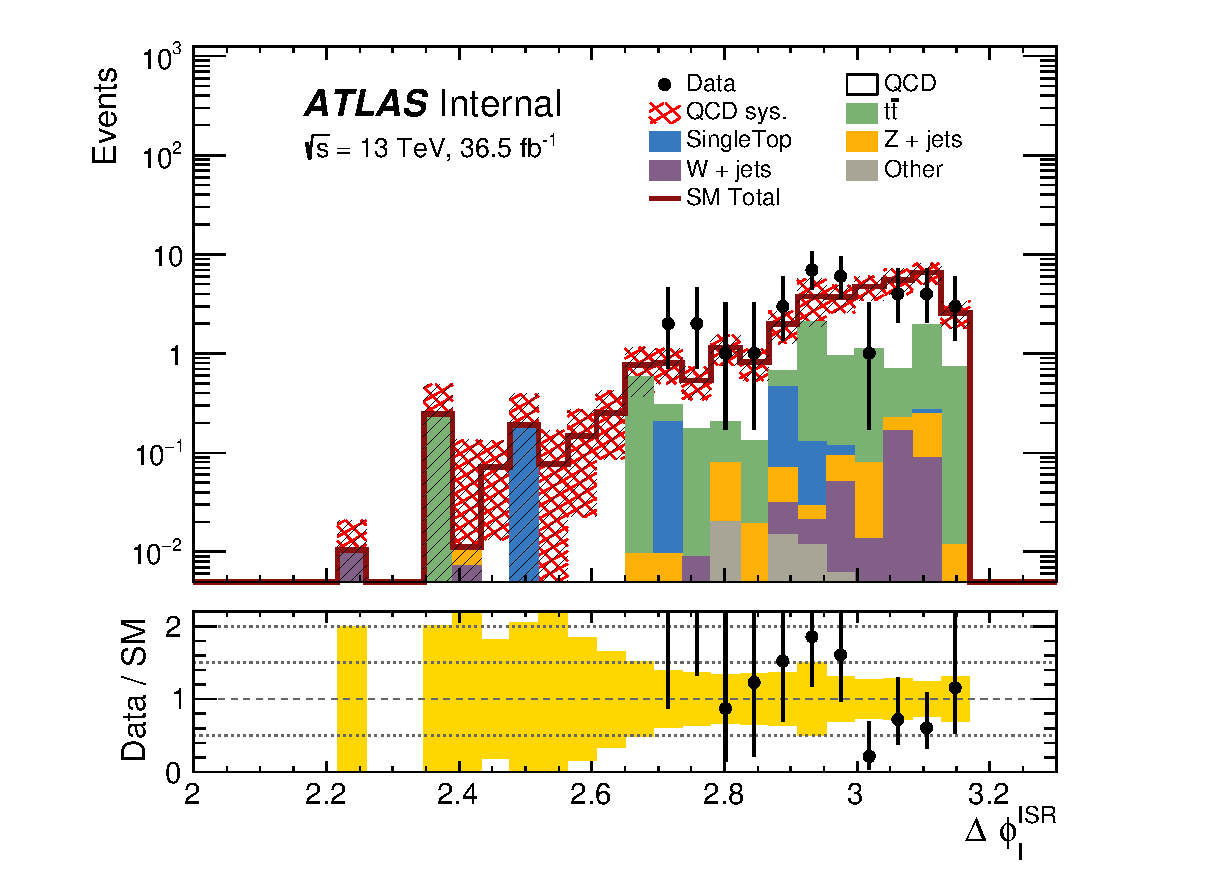
\includegraphics[width=\textwidth]{figures/QCDJetSmearing/CRQC/dphiISRI_36500.eps}
                \caption{ }
    \end{subfigure}
    \begin{subfigure}[b]{0.40\textwidth}  
    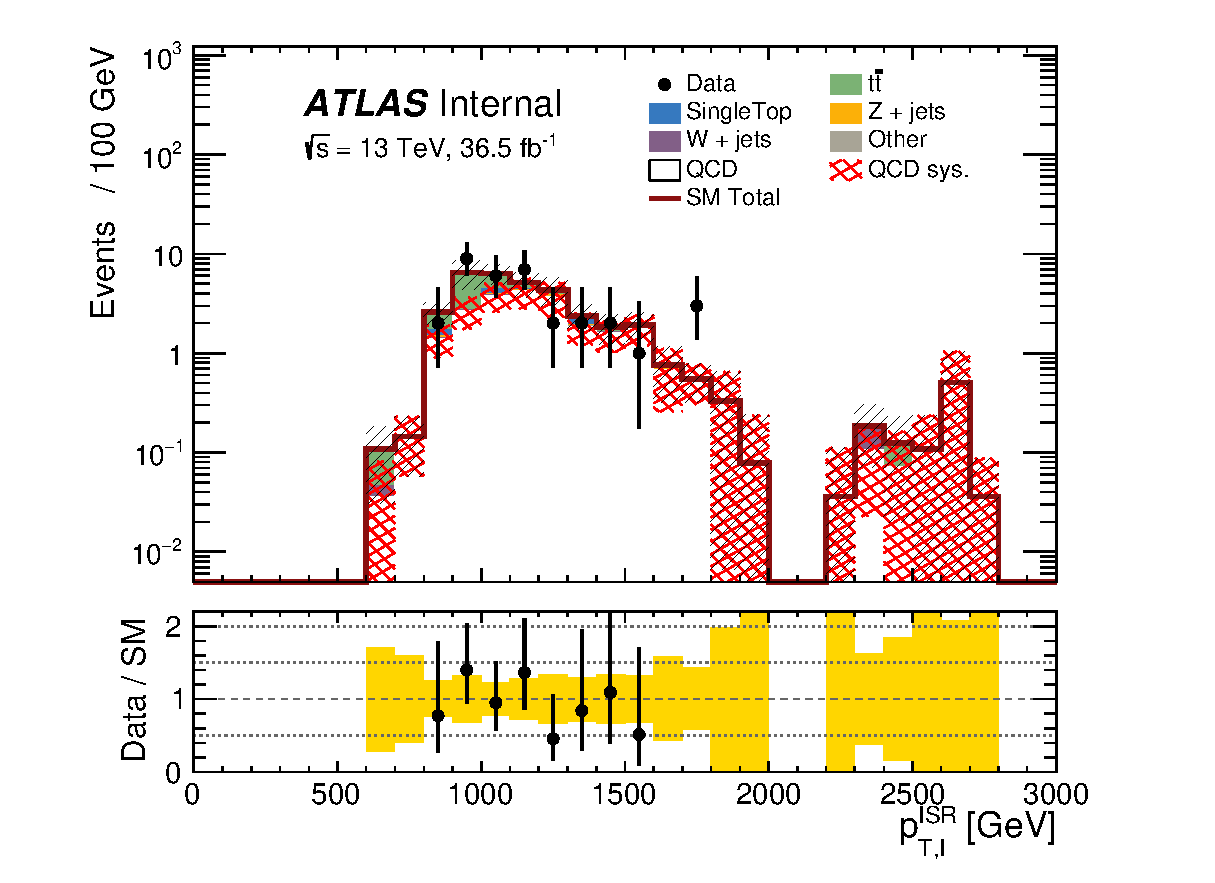
\includegraphics[width=\textwidth]{figures/QCDJetSmearing/CRQC/PTISR_36500}
                \caption{ }
    \end{subfigure}
        \begin{subfigure}[b]{0.40\textwidth}  
    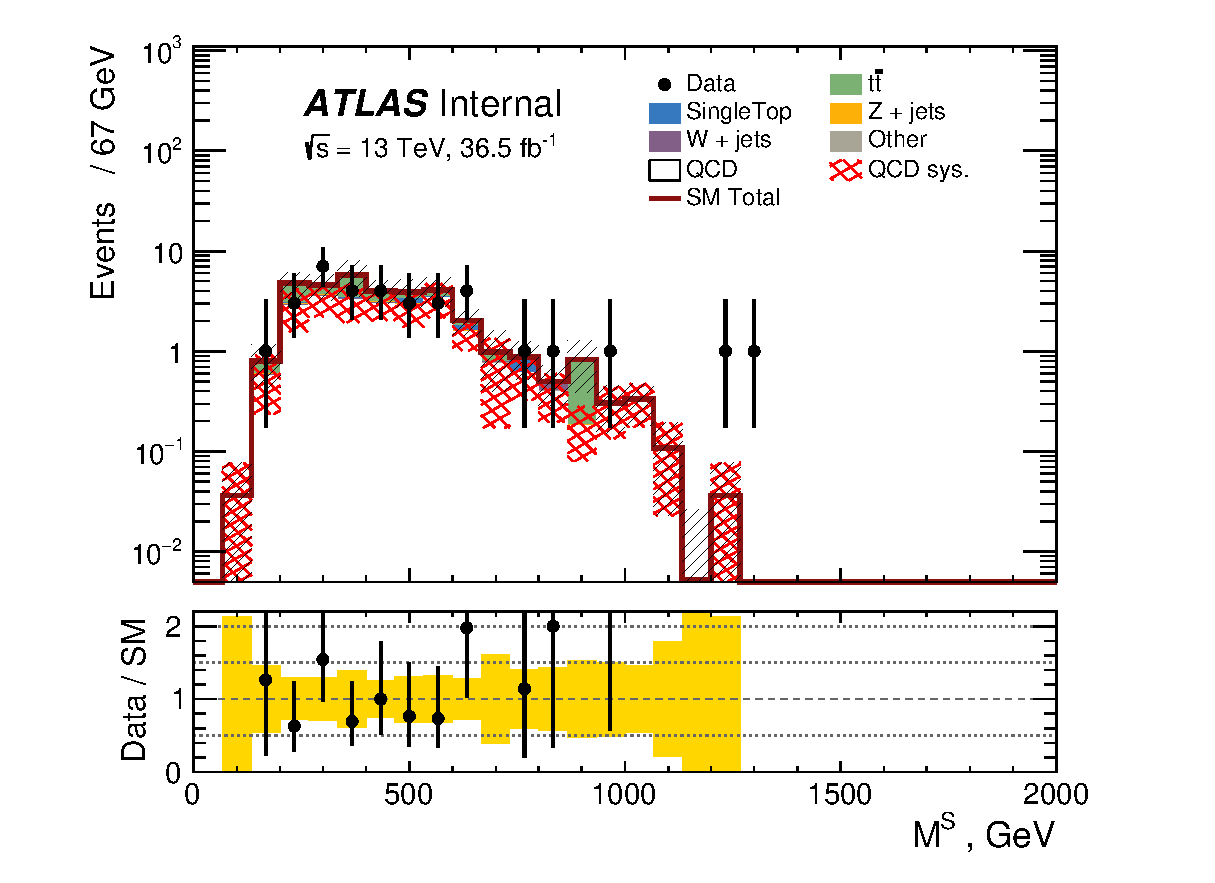
\includegraphics[width=\textwidth]{figures/QCDJetSmearing/CRQC/MV_36500}
                    \caption{ }
    \end{subfigure}
\caption[$\PTISR$, $\dphiISRI$ and $\MS$ distributions in the QCD control region]{$\PTISR$, $\dphiISRI$ and $\MS$ distributions in the QCD control region}
\label{fig:QCD:CR}
\end{center}
\end{figure}

\indent The QCD multijet prediction after normalizing to the control region can be checked in the QCD validation region defined in Table \ref{tab:QCDVR}.   The QCD validation region has the exact same kinematic selection as the signal region except a lower $\mindphijettwomet$ requirement of between $0.1$ and $0.2$.  $\RISR$ is also required to be below $0.4$ as we don't expect significant QCD contribution at higher $\RISR$.  \\

\begin{table}[h!]
  \begin{center}
    \def\arraystretch{1.4}%
    \begin{tabular}{c|c} \hline\hline
      {\bf Variable} &  QCD Validation Region  \\ \hline \hline
      \mindphijettwomet  &  [0.1,0.2]           \\  
      \nBJetS & $\ge1$ \\
      \nJetS & $\ge5$  \\
      \pTISR & $>400$ GeV \\ 
      \pTSBZero & $>40\gev$  \\ 
      \pTSFour & $>50$ GeV  \\
      \mS & $>300\gev$  \\
      \dPhiISRMET &  $>3.00$  \\ 
      \rISR  & $<0.4$ \\ \hline \hline
    \end{tabular}
  \end{center}
  \caption{QCD validation region selections, in addition to the zero lepton preselection in Table~\ref{tab:0Lcommon}. }
   \label{tab:QCDVR}
\end{table}%

\indent Data vs QCD pseudo-data distribution for the $\RISR$ and $\dphiISRI$ variables in the QCD validation region can be seen in Figure \ref{fig:QCD:CR}.  A good agreement is found between data and pseudo-data predictions. \\

\begin{figure}[!h]
\begin{center}
    \begin{subfigure}[b]{0.40\textwidth}  
    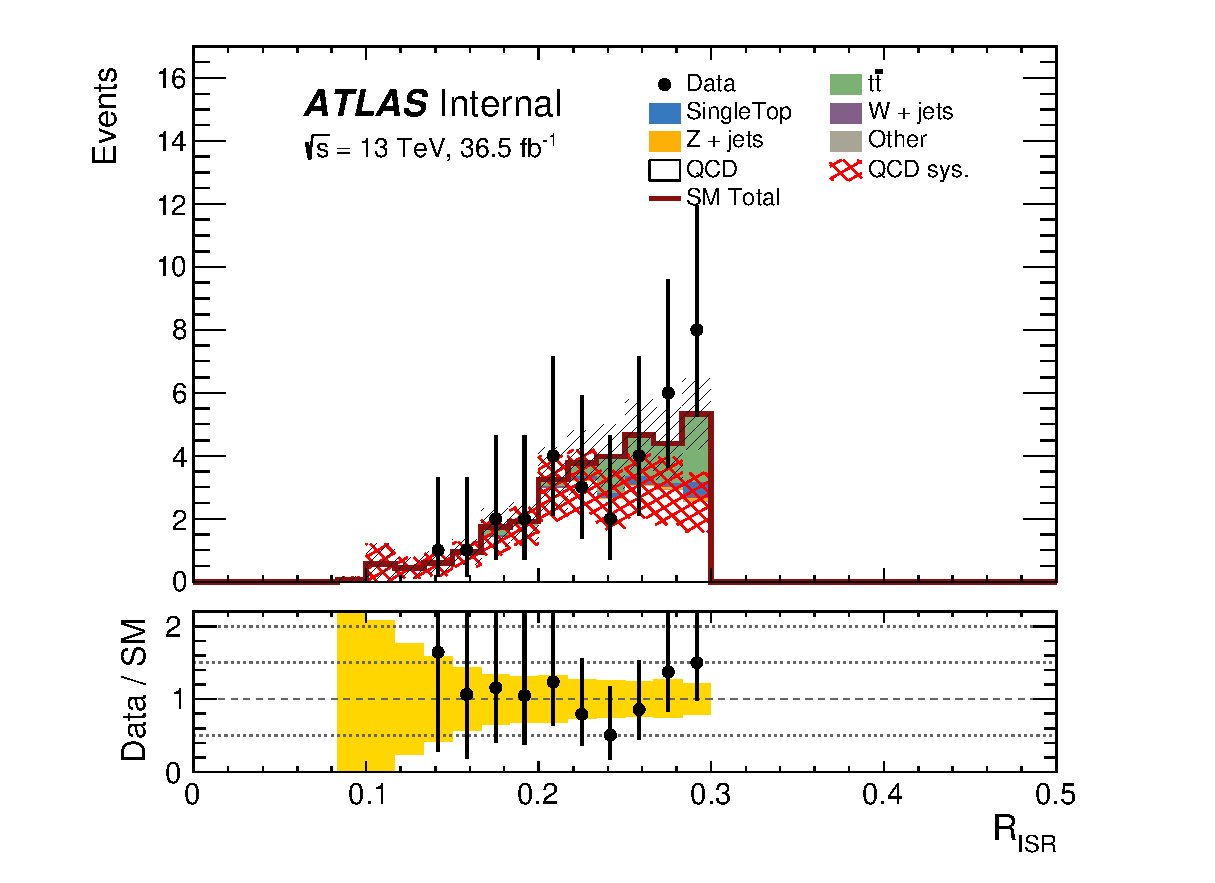
\includegraphics[width=\textwidth]{figures/QCDJetSmearing/VRqC/RISR_36500} 
                \caption{ }
    \end{subfigure}
    \begin{subfigure}[b]{0.40\textwidth}  
    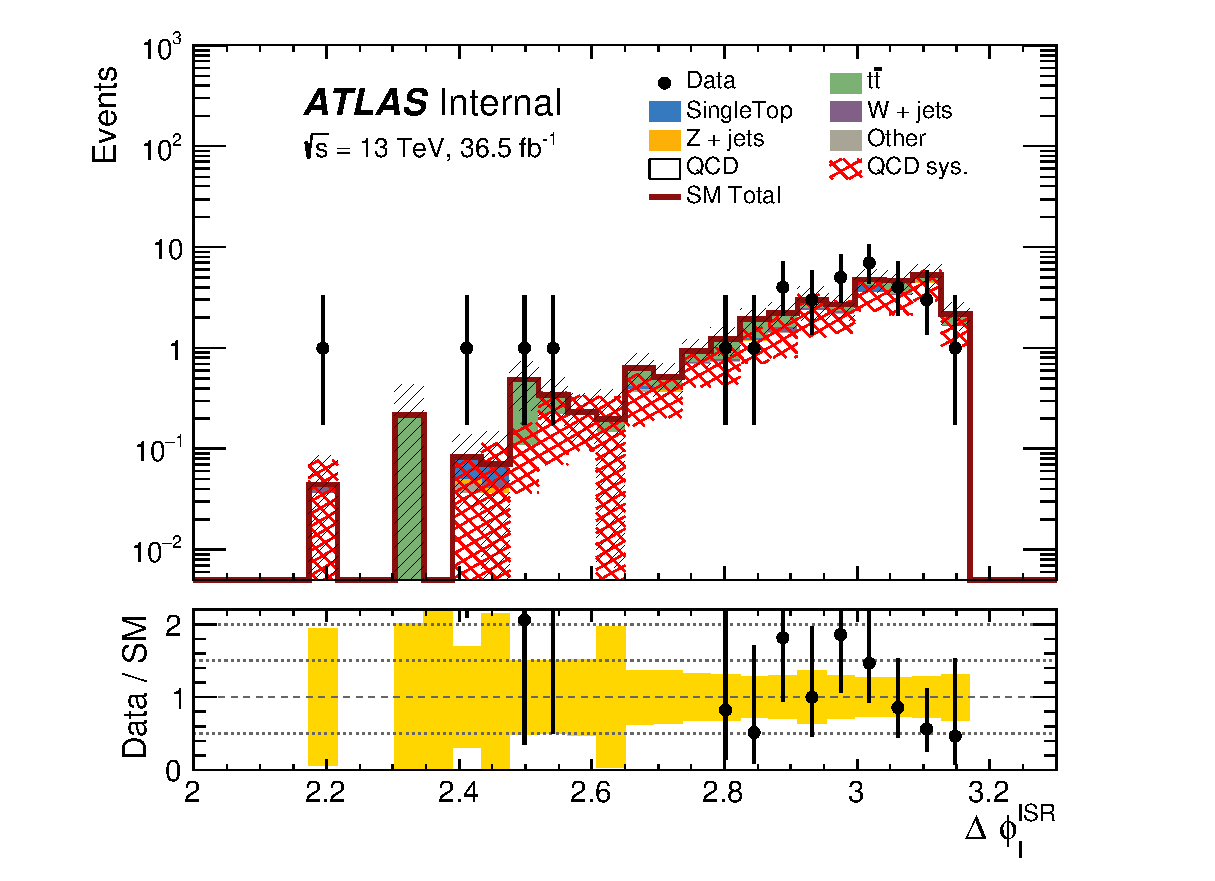
\includegraphics[width=\textwidth]{figures/QCDJetSmearing/VRqC/dphiISRI_36500.eps}
                \caption{ }
    \end{subfigure}
\caption[$\RISR$ and $\dphiISRI$ distributions in the QCD validation regions]{$\RISR$ and $\dphiISRI$ distributions in the QCD validation region.}
\label{fig:QCD:VR}
\end{center}
\end{figure}

\subsubsection{QCD prediction in the Signal Region}

\indent The predicted amount of QCD in the signal region is given by the amount of QCD pseudo-data that pass the signal region selections after normalizing to the QCD control region. The systematic uncertainty on the signal region QCD prediction is given by repeating the {\tt Jet Smearing} process with a tighter and looser set of seed event selections.  \\

\indent An upward error corresponds to using seed events requiring $\met\rm{sig.} < 0.6 + 0.2\cdot n_{\textup{n-bjets}}$ and an lower error corresponds to using seed events requiring $\met\rm{sig.} < 0.2 + 0.05\cdot n_{\textup{n-bjets}}$. QCD multijet events with better reconstructed jets tend to have a smaller $\met\rm{sig.}$. \\

\indent The expected QCD yield and uncertainty in the signal region is given in Table \ref{tab:QCDYields}.\\

\begin{table}[!h]
  \begin{center}
    \begin{tabular}{c|c|c|c} \hline\hline
SR $\RISR$ Region       & 0.3-0.4              & 0.4-0.5              & 0.5-0.6              \\ \hline
QCD expected yield & $4.56\pm2.38$ & $1.58\pm0.77$ & $0.32\pm0.17$  \\ \hline \hline
    \end{tabular}
        \begin{tabular}{c|c|c} \hline\hline
SR $\RISR$ Region         & 0.6-0.7             & 0.7-0.8 \\ \hline
QCD expected yield       & $0.04\pm0.02$ & $0.00\pm0.00$ \\ \hline \hline
    \end{tabular}
  \caption{Expected yields of the QCD multijet backgrounds in the signal region.}
  \label{tab:QCDYields}
  \end{center}
\end{table}%
